% !TEX root = ../my-thesis.tex
%
\chapter{Experimental methods}
\label{ch:methods}

\cleanchapterquote{The idea of a method that contains firm, unchanging, and absolutely binding principles for conducting the business of science meets considerable difficulty when confronted with the results of historical research.}{Paul Feyerabend}{Against Method. London: New Left Books, 1975}

The experimental methods for analysing the recorded data set of \HepProcess{\Pp\Pp} collision events are outlined in this Chapter. \Cref{sec:methods:event-reconstruction} describes the algorithms used for the reconstruction of compound physics objects. The statistical techniques used to obtain results from fits of the statistical model to data are described in \Cref{sec:methods:statistics}. The RECAST framework, which enables faithful and efficient reinterpretation of searches, is introduced in \Cref{sec:methods:recast}.

\section{Event reconstruction}
\label{sec:methods:event-reconstruction}
\subsection{Introduction}
\label{sec:methods:event-reconstruction:intro}
The various sub-systems of the ATLAS detector record detailed information about the \HepProcess{\Pp\Pp} collisions, which occur in the interaction region. The elementary detector signatures are the hits in the sensitive tracking detector planes and the energy deposits in the calorimeters. These measurements serve as inputs for sophisticated reconstruction algorithms, which define compound physical objects, such as electrons, photons, muons, tau leptons, jets, and missing transverse momentum. These compound physical objects are used to define the selection requirements in the searches for dark matter and to construct discriminating observables for the statistical analysis.

The object reconstruction is subject to inefficiencies in the particle identification and afflicted with systematic uncertainties due to various detector effects. The reconstructed kinematic properties of the compound physical objects can deviate from their true value for the same reasons. These discrepancies can be reduced to some extent by employing calibration methods. In the ATLAS collaboration, the standard recommendations for object identification, reconstruction, calibration, and evaluation of the associated systematic uncertainties are centrally provided by the Combined Performance (CP) groups.


\subsection{Reconstruction of basic objects}
\label{sec:methods:event-reconstruction:basic}
All reconstructed physics objects are based on reconstructed tracks, vertices, and topological clusters.

\textbf{Tracks} are reconstructed by connecting the hits in different layers of the ID. Their momentum and charge can be inferred from their deflection in the solenoidal magnetic field.
The tracks are parametrised, as shown in \Cref{fig:methods:event-reconstruction:tracks:parametrisation}, by a set of five parameters
\begin{itemize}
	\item the transverse and longitudinal impact parameters \(d_{0}\) and \(z_{0}\),
	\item the azimuthal and polar angles \(\varphi\) and \(\theta\), and
	\item the ratio of charge and transverse momentum \(q / \pt\).
\end{itemize}
Tracks are reconstructed by a set of tracking algorithms~\cite{ATLAS-CONF-2012-042,PERF-2015-08}.
Two approaches --- an ``inside-out'' algorithm, mostly sensitive to primary charged particles produced in the \HepProcess{\Pp\Pp} interaction, and an ``outside-in'' algorithm, mostly sensitive to secondary decay products --- are employed to ensure high reconstruction efficiency. The ``inside-out'' algorithm considers seeds containing three hits in the silicon PXD and SCT detectors and extends the track seed to the TRT using a combinatorial Kalman filter~\cite{Frhwirth1987} to add hits further away from the interaction point. The ``outside-in'' algorithm considers TRT track segments and extrapolates them to the vicinity of the interaction point by adding hits in the silicon detectors, which have not been associated with tracks yet. All ID tracks are required to satisfy \(\pt > \SI{0.4}{\giga\electronvolt}\) and \(\abs{\eta} < 2.4\). The impact parameter resolution is shown in \Cref{fig:methods:event-reconstruction:tracks:impactparameter-resolution}.
In addition to the tracks in the ID, the muon reconstruction employs tracks recorded by the MS. These are reconstructed by dedicated algorithms based on Hough transforms or iterative combination of hits~\cite{Nicolaidou2008}.

\begin{figure}[htbp]
	\centering
	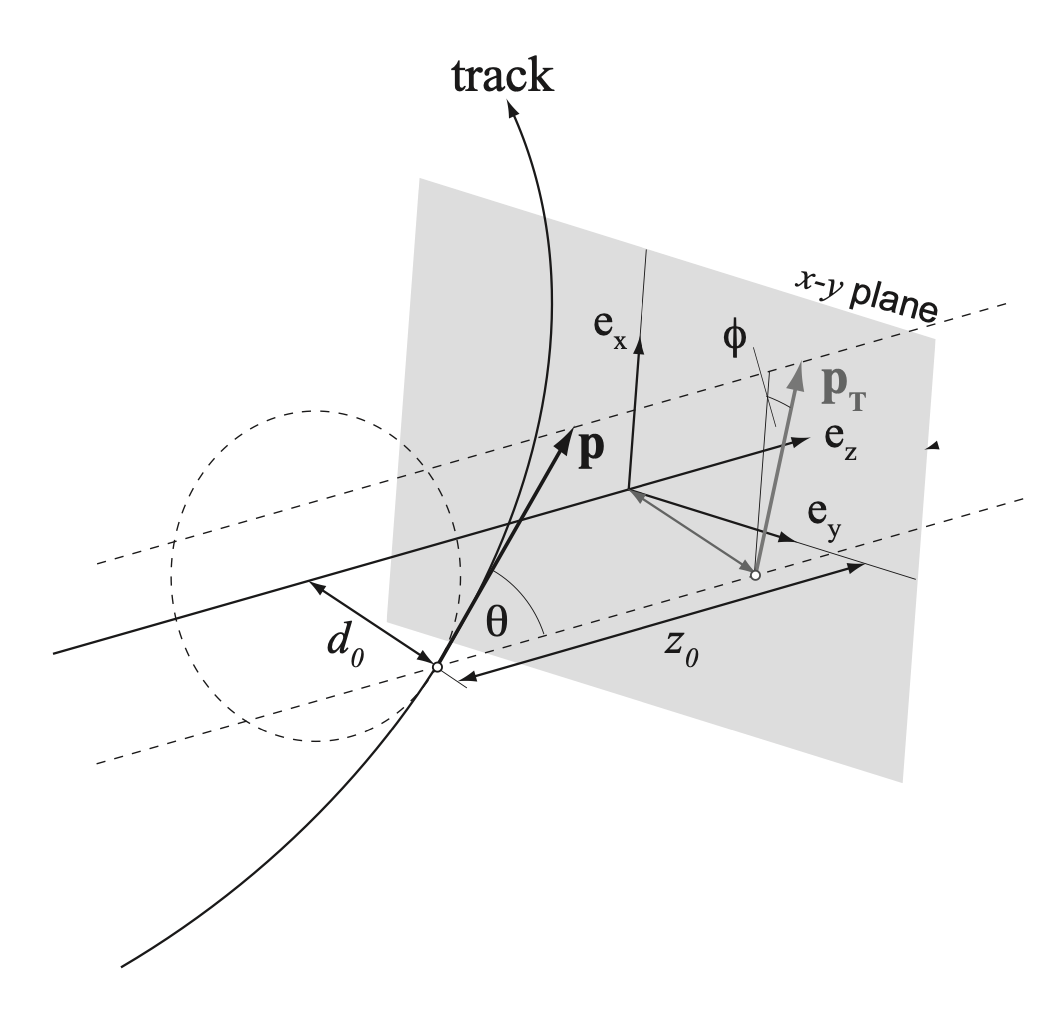
\includegraphics[width=0.73\textwidth]{figures/methods/track.png}
	\caption{A track parametrised with respect to the nominal \(z\)-axis through the azimuthal angle \(\varphi\), the polar angle \(\theta\), the charged inverse momentum \(q / p\), and the transverse and longitudinal impact parameters \(d_{0}\) and \(z_{0}\). Figure reproduced from Ref.~\cite{Cornelissen2007}.}
	\label{fig:methods:event-reconstruction:tracks:parametrisation}
\end{figure}

\begin{figure}[htbp]
	\centering
	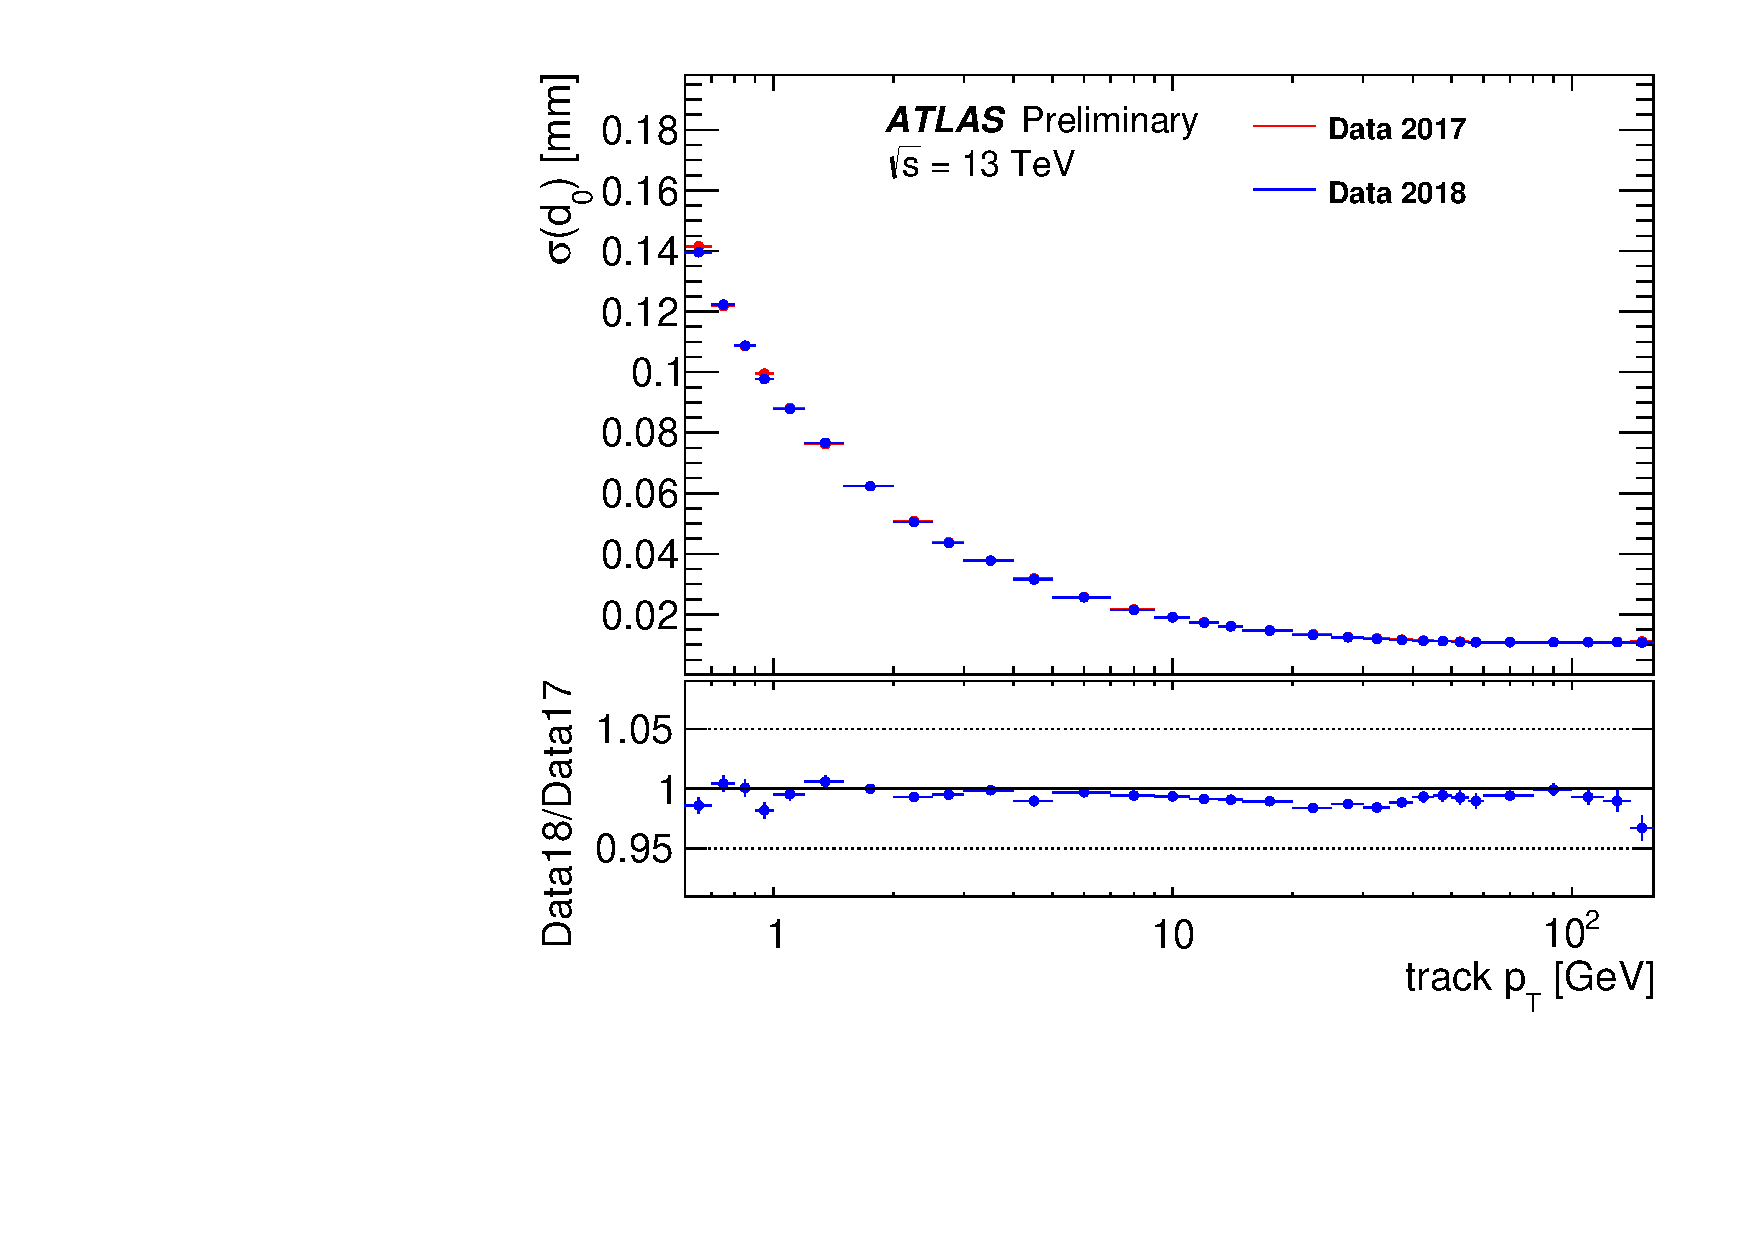
\includegraphics[width=0.45\textwidth]{figures/methods/tracking_resolution_d0.pdf}
	\hfill
	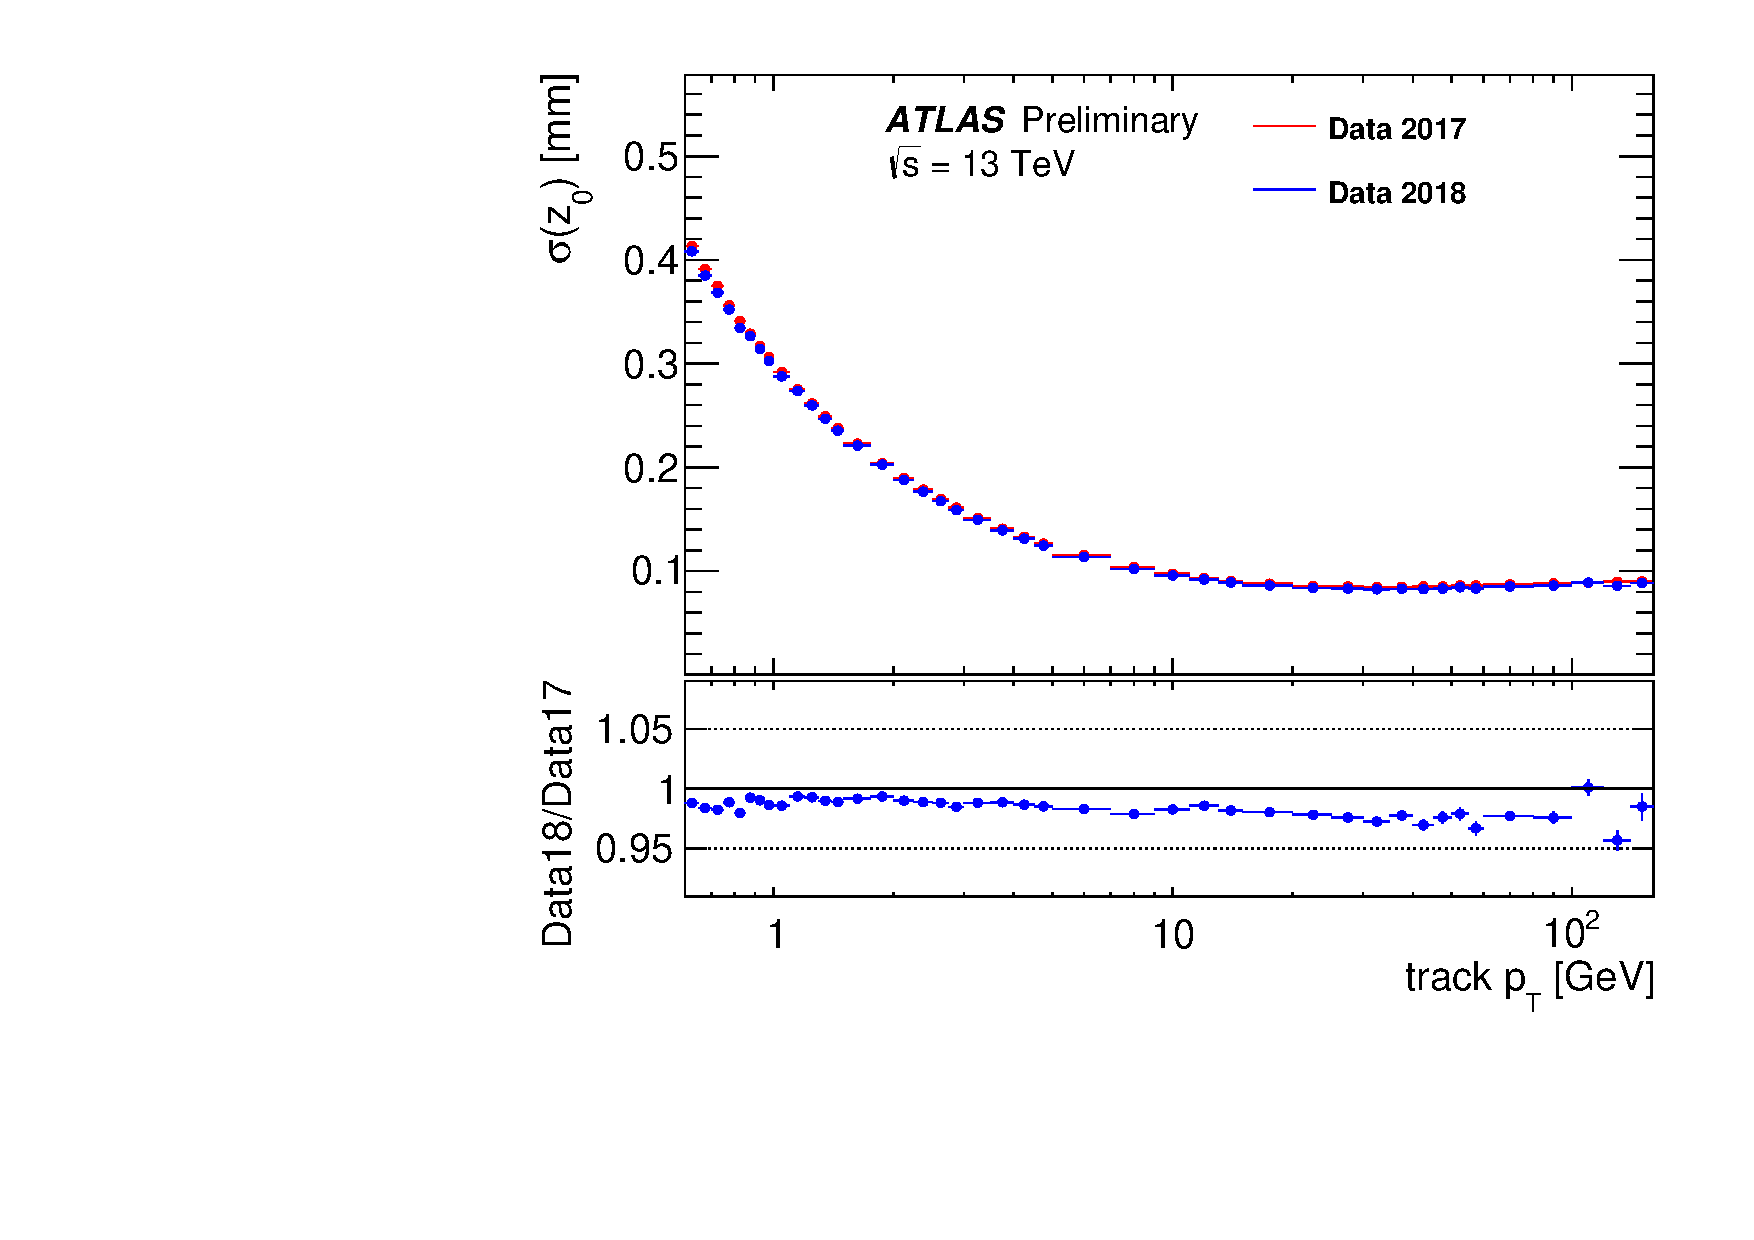
\includegraphics[width=0.45\textwidth]{figures/methods/tracking_resolution_z0.pdf}
	\caption{Resolution of the transverse impact parameter \(d_{0}\) and the longitudinal impact parameter \(z_{0}\) of tracks associated with jets with \(\pt > \SI{20}{\giga\electronvolt}\), measured in \HepProcess{\Pp\Pp} collision data recorded in 2017 and 2018 with dijet triggers. Figure reproduced from Ref.~\cite{IDTR-2018-008}.}
	\label{fig:methods:event-reconstruction:tracks:impactparameter-resolution}
\end{figure}

\textbf{Vertices} are defined as points at which either a \HepProcess{\Pp\Pp} interaction or a decay takes place. The iterative reconstruction of vertices employs tracks and consists of two steps~\cite{Boutle2017}.
\begin{enumerate}
	\item Vertex finding. The vertices in a collision event are reconstructed using tracks satisfying certain quality criteria, including \(\abs{d_{0}} < \SI{4}{\milli\meter}\) and requirements on the impact parameter resolution \(\sigma(d_{0}) < \SI{5}{\milli\meter}\) and \(\sigma(z_{0}) < \SI{10}{\milli\meter}\). The seed position for the first vertex is defined by the transverse coordinates of the beam spot and the \(z\)-coordinates or tracks at their points of closest approach to the beam spot.
	All vertices require at least two associated tracks.
	\item Vertex fitting. The tracks and the seed are used to estimate the best vertex position with a fit based on an iterative annealing procedure. In each iteration of the fit, the weights of less compatible tracks are decreased, to determine the best vertex position.
\end{enumerate}
The primary vertex (PV) is the point at which a hard scattering process in the \HepProcess{\Pp\Pp} interaction occurred. It is reconstructed as the vertex with the largest sum of squared transverse momenta of all tracks associated with it. \Cref{fig:methods:event-reconstruction:vertex:performance} shows the vertex performance in two runs of 2018 \HepProcess{\Pp\Pp} data with different average number of interactions per bunch crossing.

\begin{figure}[htbp]
	\centering
	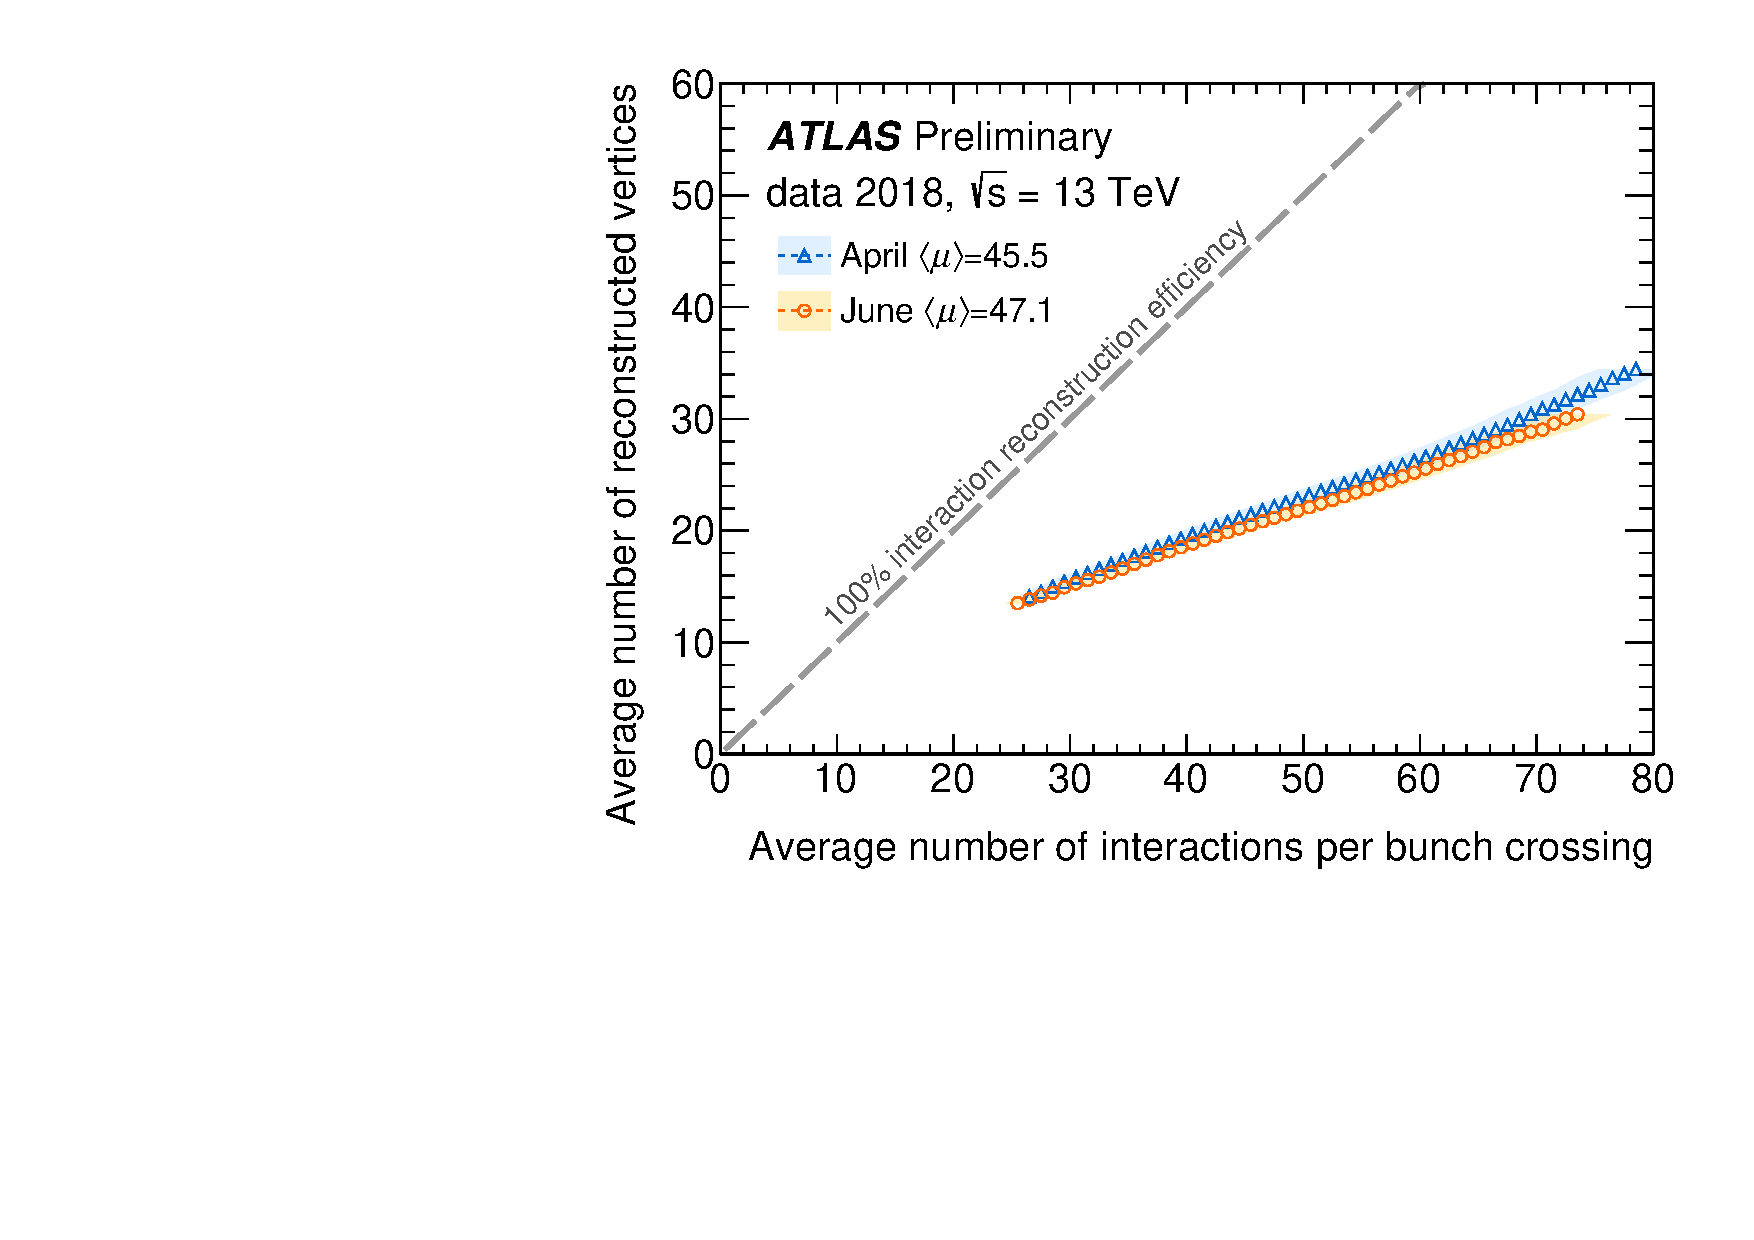
\includegraphics[width=0.75\textwidth]{figures/methods/vertex_efficiency.pdf}
	\caption{Vertex performance in 2018 \HepProcess{\Pp\Pp} data, indicated by the number of reconstructed vertices in dependence of the average number of interactions per bunch crossing. Figure reproduced from Ref.~\cite{IDTR-2018-008}.}
	\label{fig:methods:event-reconstruction:vertex:performance}
\end{figure}


\textbf{Topological clusters} are groups of topologically connected energy deposits in neighbouring calorimeter cells due to incident particles. Their reconstruction~\cite{PERF-2014-07} is seeded by energy deposits which are significantly greater than the expected noise due to the detector electronics and pile-up events. The reconstruction is based on the cell signal significance \(\xi = E_{\text{cell}} / \sigma(E_{\text{cell}})\), which is defined as the ratio of the detector signal \(E_{\text{cell}}\) and the expected noise \(\sigma(E_{\text{cell}})\) on the electromagnetic scale. All calorimeter cells adjacent to the seed cells, which satisfy certain noise-suppression thresholds, are iteratively added to form ``proto-clusters''. These ``proto-clusters'' are subsequently split if they contain two or more local maximums of the detector signal with \(E_{\text{cell}} > \SI{500}{\mega\electronvolt}\) to separate individual showers.
The clusters are parametrised by the azimuthal and polar angles defined by the energy-weighted barycentre of the associated calorimeter cells and by the cluster energy.
The cluster energy can be calibrated to different scales to adequately describe the physical objects initiating the shower in the calorimeters~\cite{PERF-2014-02}.
\begin{itemize}
	\item Electromagnetic (EM) scale calibration. Topological clusters in their basic definition are reconstructed at the EM scale to describe particles depositing their energy in the calorimeter via electromagnetic showers.
	\item Local Calibration Weighting (LCW) calibration. This alternative calibration~\cite{PERF-2011-03} takes into account the response of the calorimeter to hadrons produced in the interaction point. Clusters are classified either as electromagnetic or hadronic before the appropriate energy corrections derived from single pion MC simulations are applied. The LCW calibration can improve the energy resolution of reconstructed jets in comparison to jets based on EM-scale clusters.
\end{itemize}

\subsection{Electrons}
\label{sec:methods:event-reconstruction:electrons}
Electrons passing the ATLAS detector leave a track in the ID and initiate an electromagnetic shower in the high-granularity EM calorimeter. The electron candidates are reconstructed based on the combined information of the two sub-detectors.
The performance of the electron reconstruction, identification, and isolation algorithms is evaluated in data and simulated MC samples using electrons from \HepProcess{\PZ \to \Pem \Pep} and \HepProcess{\PJgy \to \Pem \Pep} decays.

\subsubsection{Electron reconstruction}
Electron candidates are reconstructed by matching reconstructed tracks to clusters in the EM calorimeter. The coverage of the ID limits the electron reconstruction to \(\abs{\eta} < 2.47\). The path of an electron through the detector is shown in \Cref{fig:methods:event-reconstruction:electrons:path}.

\begin{figure}[htbp]
	\centering
	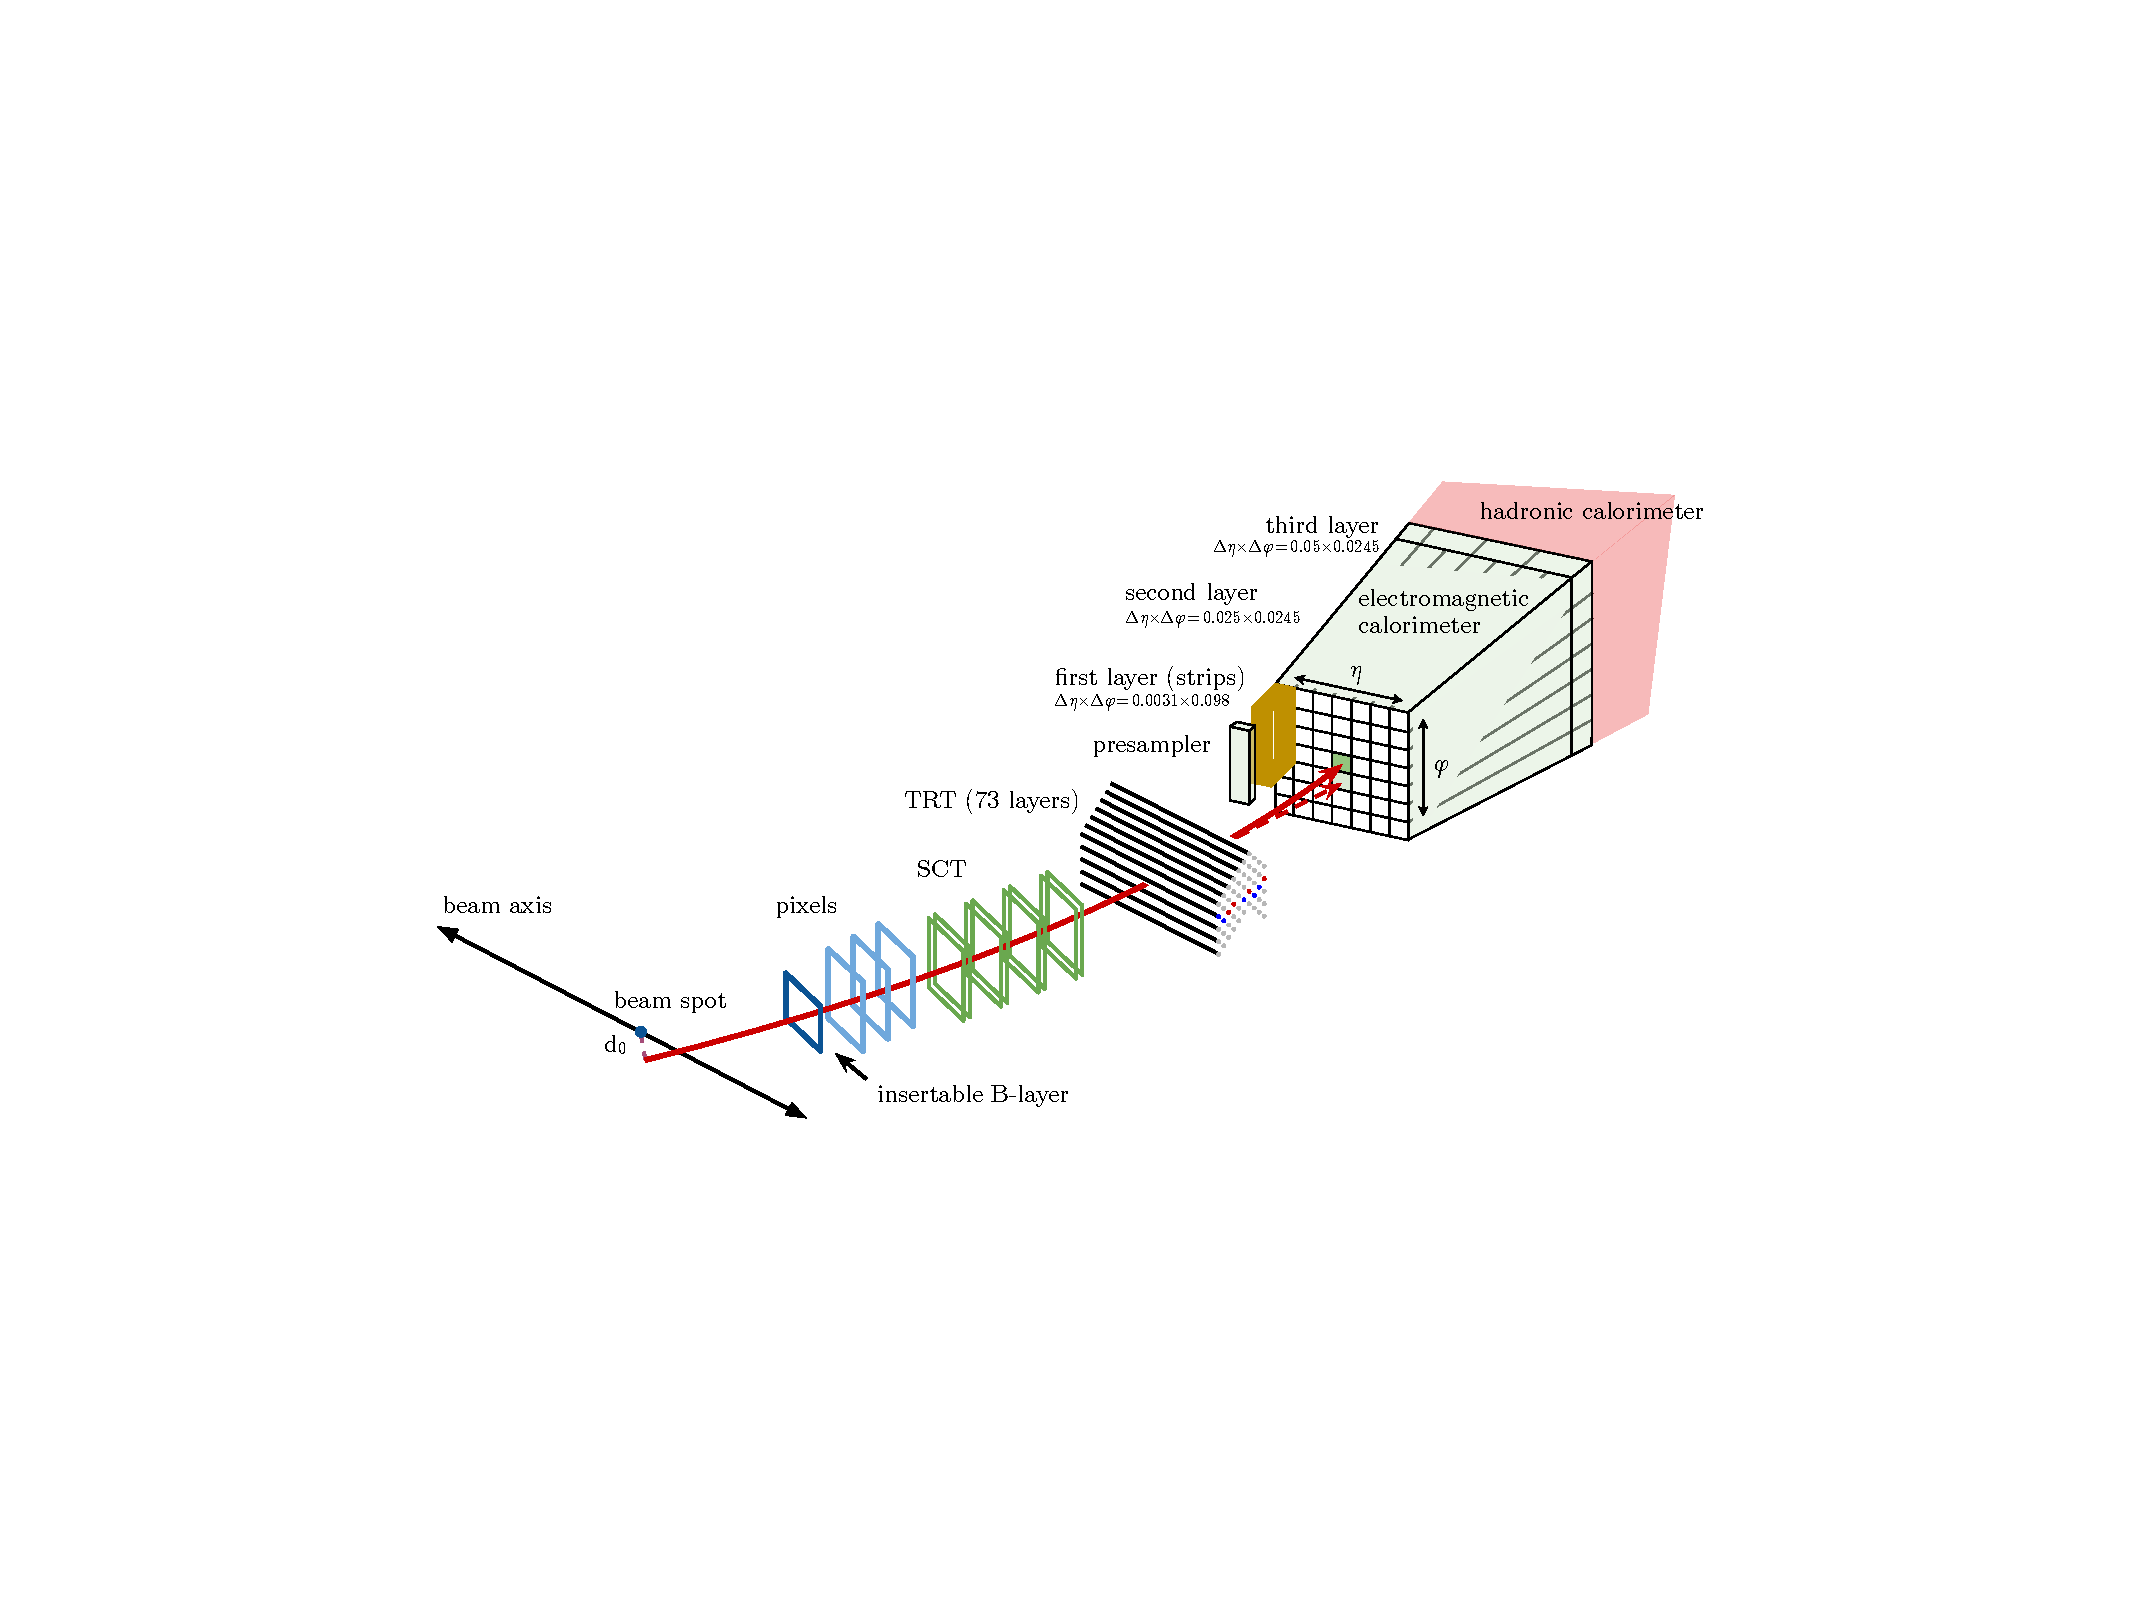
\includegraphics[width=0.95\textwidth]{figures/methods/electron.pdf}
	\caption{Schematic illustration of an electron's trajectory (red) through the detector, first traversing the tracking system comprised of PXD detectors, SCT detectors and lastly the TRT, and then enters the EM calorimeters. The dashed trajectory (red) illustrates the path of a photon radiated off the electron due to interactions with the detector material. Figure reproduced from Ref.~\cite{PERF-2017-01}.}
	\label{fig:methods:event-reconstruction:electrons:path}
\end{figure}

The electron reconstruction~\cite{PERF-2017-01} starts from fixed-size seed clusters, which are selected by a sliding-window algorithm. The inputs to the algorithms are towers of calorimeter cells in the first three calorimeter layers, which have a granularity of \(\Delta \eta \times \Delta \varphi = 0.025 \times 0.025\).
The algorithm considers seeds composed of \(N_{\eta} \times N_{\varphi} = 3 \times 5\) towers of EM calorimeter cells, which are required to have a minimal energy deposit of \(E_{\text{T}} > \SI{2.5}{\giga\electronvolt}\).

ID tracks are matched to the clusters using the distance measure \(\Delta R\) between the position of the track extrapolated to the middle layer of the calorimeter and the cluster barycentre. The tracks are re-fitted with the Gaussian Sum Filter (GSF)~\cite{ATLAS-CONF-2012-047} algorithm to account for Bremsstrahlung effects. The resulting electron candidate consists of a cluster seed, which is successfully matched to at least one track.

In the 2017--2018 data taking campaign, new electron reconstruction algorithms are employed~\cite{ATL-PHYS-PUB-2017-022,EGAM-2018-01}. These algorithms replace the electron reconstruction based on fixed-size windows with a dynamic approach based on variable-size topological clusters.

\subsubsection{Electron identification}
The electron identification (ID) algorithm discriminates between electron candidates from signal processes, such as prompt production in the hard-scattering vertex or from the decay of heavy resonances, and background-like objects, such as hadronic jets or converted photons. A likelihood-based approach (LH) is employed, which considers the information provided by clusters and tracks, such as the resolution parameters of the associated tracks and the calorimeter shower shape. The LH based discriminant and the number of hits in the track are used to calculate the probability of an electron candidate being either an electron from signal processes or a background-like object.

Three electron ID operating points (OPs) with increasing background rejection are defined.
The \textsc{Loose} OP corresponds to an average electron identification efficiency of \SI{93}{\percent}.
Similarly, the \textsc{Medium} and \textsc{Tight} OPs correspond to efficiencies of \SI{88}{\percent} and \SI{80}{\percent}, respectively.
These points are inclusive, meaning that the \textsc{Tight} electrons are a subset of the \textsc{Medium} electrons and the \textsc{Medium} electrons are a subset of the \textsc{Loose} electrons. In addition, the \textsc{LooseAndBLayer} OP is defined as a variation of the \textsc{Loose} OP with the additional requirement of at least one hit in the innermost layer of the PXD detector.
Out of these definitions, \textsc{Loose} and \textsc{LooseAndBLayer} electrons are considered in the searches for dark matter presented in this dissertation.

The electron identification efficiency in bins of \(E_{\text{T}}\) and \(\eta\) is shown in \Cref{fig:methods:event-reconstruction:electrons:identification}. The identification efficiency gradually increases from low to high \(E_{\text{T}}\). In the range \(\SI{20}{\giga\electronvolt} < E_{\text{T}} < \SI{50}{\giga\electronvolt}\), the \textsc{Medium} and \textsc{Tight} OPs have an improved rejection of background processes by \num{2.0} and \num{3.5}, respectively, with respect to the \textsc{Loose} OP.
\begin{figure}[htbp]
    \centering
    \begin{subfigure}{1.\textwidth}
      \centering
      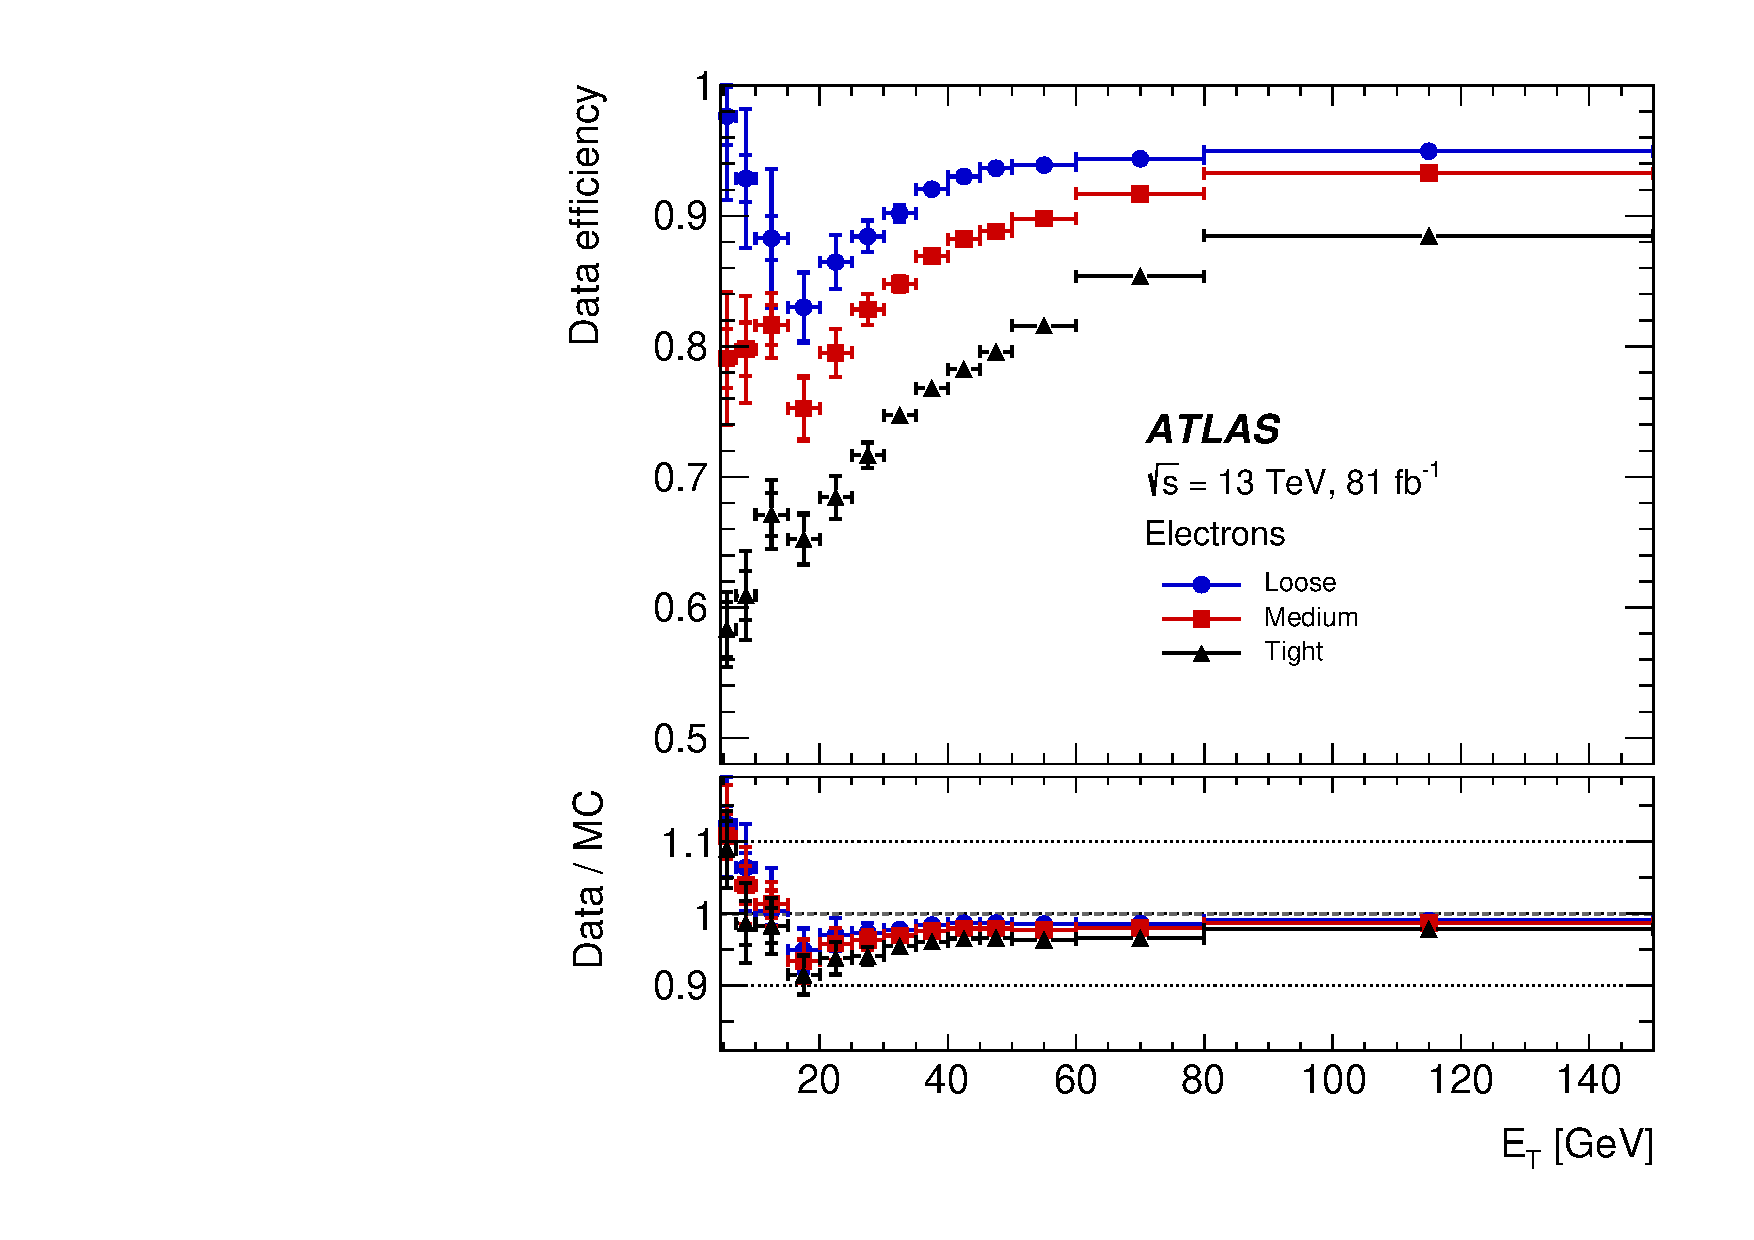
\includegraphics[width=0.79\textwidth]{figures/methods/electron_id_et.pdf}
      \caption{Electron identification efficiency in bins of \(E_{\text{T}}\).}
      \label{fig:methods:event-reconstruction:electrons:identification:et}
    \end{subfigure}
    \\
    \begin{subfigure}{1.\textwidth}
      \centering
      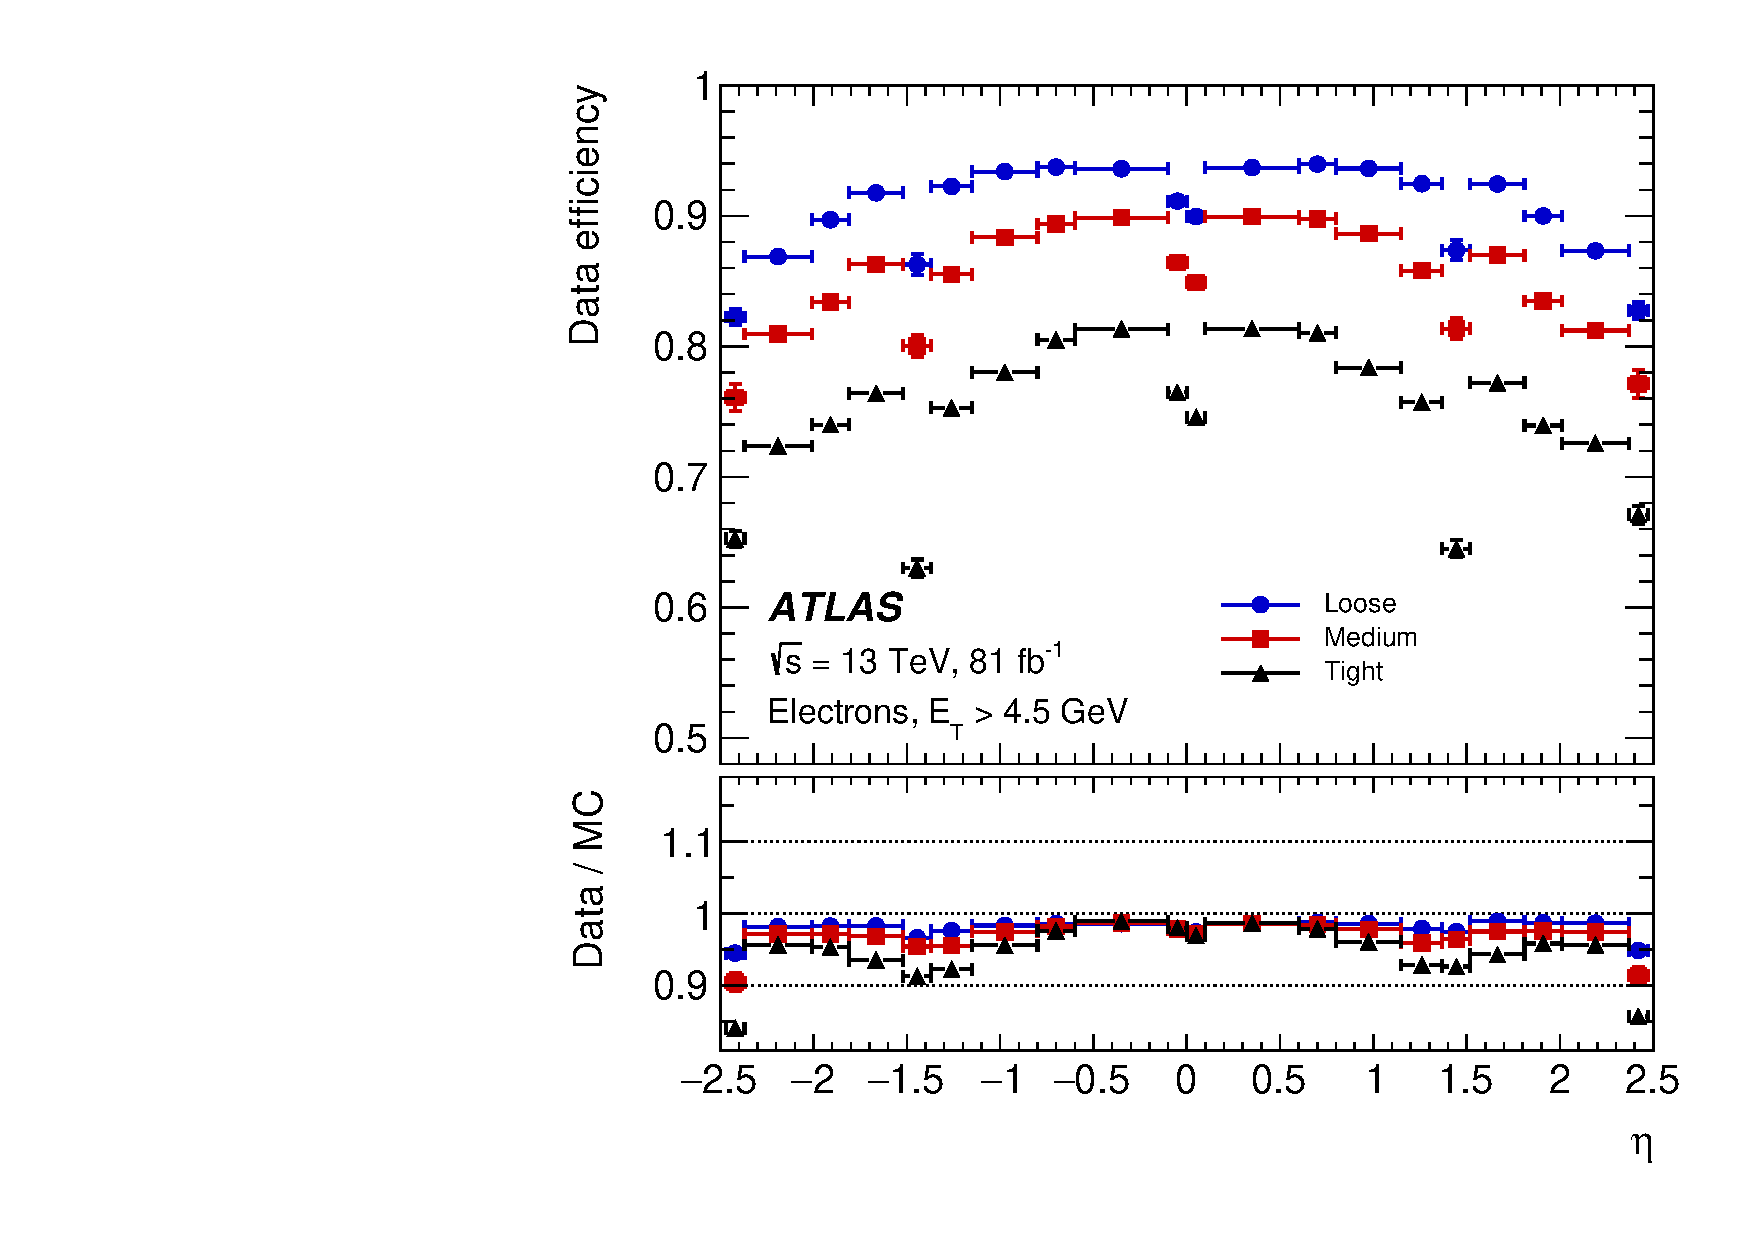
\includegraphics[width=.79\textwidth]{figures/methods/electron_id_eta.pdf}
      \caption{Electron identification efficiency in bins of \(\eta\).}
      \label{fig:methods:event-reconstruction:electrons:identification:eta}
    \end{subfigure}
    \caption{Electron identification efficiencies for the different operating points \textsc{Loose}, \textsc{Medium}, and \textsc{Tight}. Figures reproduced from Ref.~\cite{EGAM-2018-01}.}
    \label{fig:methods:event-reconstruction:electrons:identification}
\end{figure}

\subsubsection{Electron isolation}
The electron isolation algorithm provides additional information to discriminate between electrons from signal processes and background-like objects. Typically, the latter are characterised by comparatively larger activity in an area of \(\eta \times \varphi\) surrounding the electron candidate.
The amount of activity in the vicinity of the electron is quantified by variables summing the transverse energy of clusters or transverse momenta of tracks in a cone of radius \(\Delta R\) around the direction of the electron, excluding the electron itself.

Two types of variables are defined.
\begin{itemize}
	\item The track isolation variable \(p_{T}^{\text{varcone}, 0.2}\) is defined as the sum of the transverse momenta of all tracks in a cone of variable size \(R = \min \{0.2, \SI{10}{\giga\electronvolt} / E_{\text{T}}\}\) around the direction of the electron candidate with transverse energy \(E_{\text{T}}\).
	The \(p_{T}^{\text{varcone}, 0.3}\) variable is defined similarly.
	\item The calorimeter \(E_{T}^{\text{cone}, 0.2}\) isolation variable is defined as the sum of the transverse energies of all calorimeter cells, which are calibrated to the electromagnetic cell, in a cone with fixed size \(R=0.2\) around the electron.
\end{itemize}

Various electron isolation OPs are defined. These can be based either on targeting a fixed value of the isolation efficiency dependent on \(E_{\text{T}}\) and uniform in \(\eta\) (``Gradient'') or by imposing fixed requirements on the value of the isolation variable (``Fixed Cut'').

The electron isolation efficiency for various OPs in bins of \pt and \(\eta\) is shown in \Cref{fig:methods:event-reconstruction:electrons:isolation}.
\begin{figure}[htbp]
    \centering
    \begin{subfigure}{1.\textwidth}
      \centering
      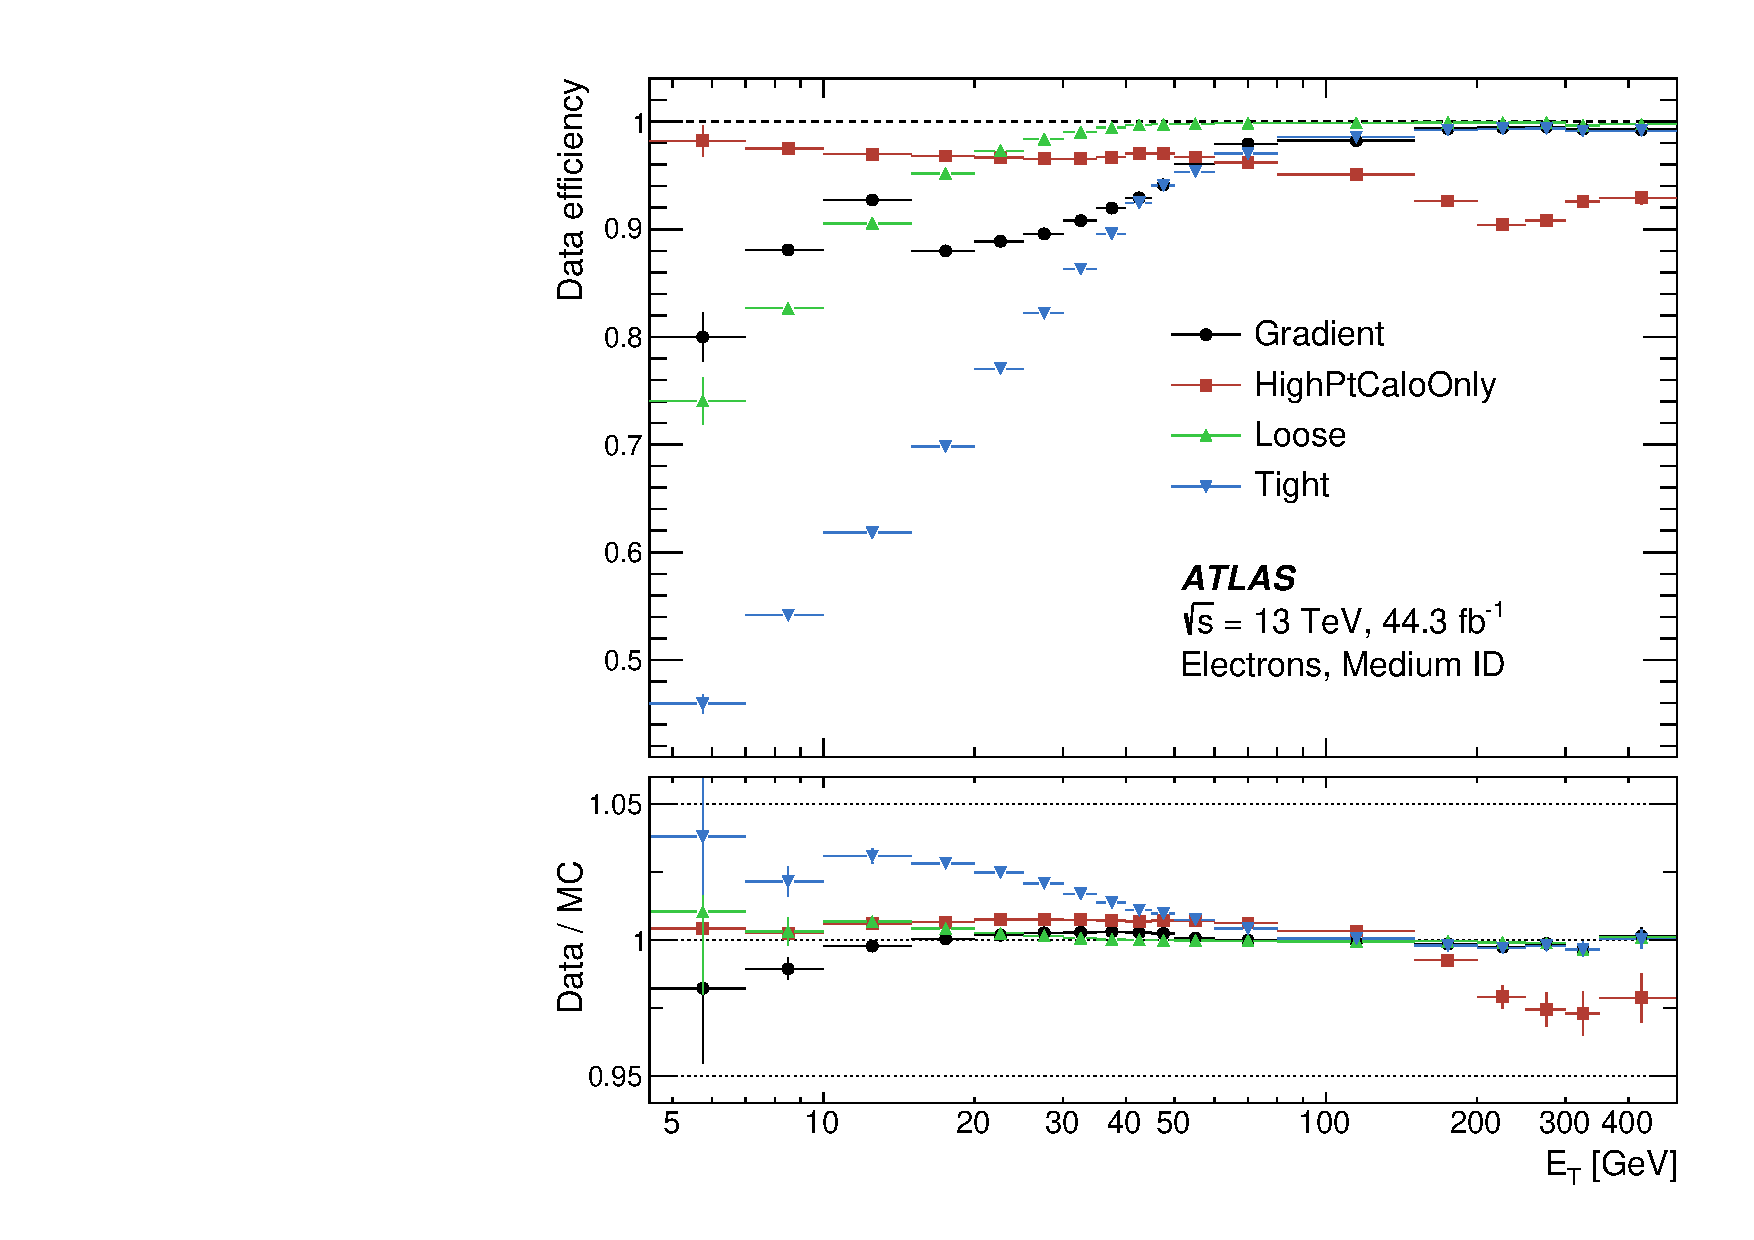
\includegraphics[width=0.79\textwidth]{figures/methods/electron_iso_et.pdf}
      \caption{Electron isolation efficiency in bins of \(E_{\text{T}}\).}
      \label{fig:methods:event-reconstruction:electrons:isolation:et}
    \end{subfigure}
    \\
    \begin{subfigure}{1.\textwidth}
      \centering
      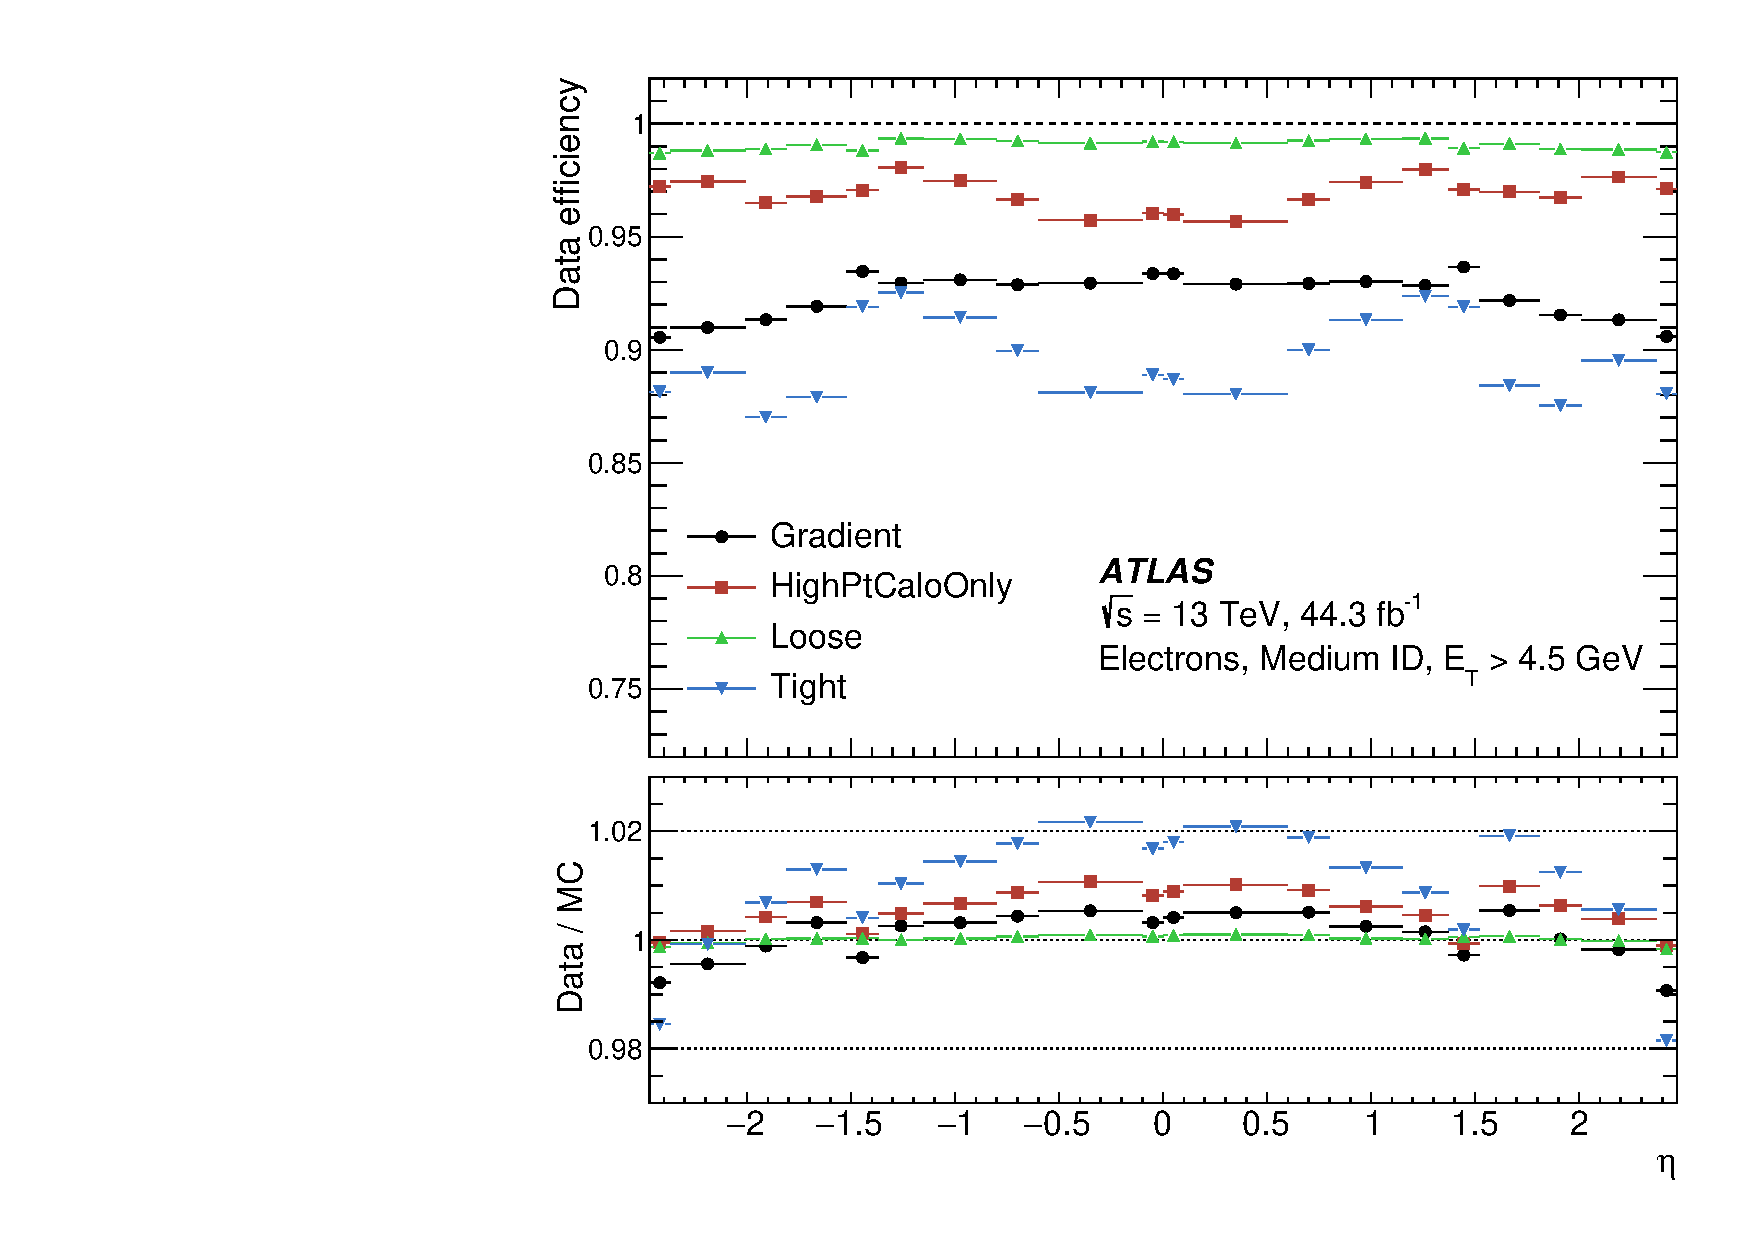
\includegraphics[width=.79\textwidth]{figures/methods/electron_iso_eta.pdf}
      \caption{Electron isolation efficiency in bins of \(\eta\).}
      \label{fig:methods:event-reconstruction:electrons:isolation:eta}
    \end{subfigure}
    \caption{Electron isolation efficiencies for the fixed cut OPs ``Loose'', ``Tight'', and ``HighPtCaloOnly'', as well as for the ``Gradient'' OP. Figures reproduced from Ref.~\cite{EGAM-2018-01}.}
    \label{fig:methods:event-reconstruction:electrons:isolation}
\end{figure}


\subsection{Muons}
\label{sec:methods:event-reconstruction:muons}
Muons traversing the ATLAS detector leave a track in the ID and the MS, as they pass the calorimeters with only minimal energy loss. The muon trajectory is reconstructed independently in the ID and the MS. Then, the two measurements are combined, potentially supplemented with calorimeter information, to form muon candidates.

The performance of the muon reconstruction, identification, and isolation algorithms is evaluated in data and simulated MC samples using muons from \HepProcess{\PZ \to \Pgmm \Pgmp} and \HepProcess{\PJgy \to \Pgmm \Pgmp} decays.

\subsubsection{Muon reconstruction}
The muon reconstruction~\cite{PERF-2015-10,ATLAS-CONF-2020-030} is performed separately in the ID and the MS. While the muon reconstruction in the ID is identical to that of other charged particles (c.f. \Cref{sec:methods:event-reconstruction:basic}), it based on a combinatorial search algorithm in the MS. The algorithm constructs the track candidates from at least two matching track segments, which are identified in the individual layers of the MS by pattern finding algorithms.

Six types of muons are reconstructed depending on the available sub-detector information and based on different reconstruction algorithms. The reconstructed muon types are combined (CB) muons, silicon-associated forward (SiF) muons, inside-out combined (IO) muons, segment-tagged (ST) muons, calorimeter-tagged (CT) muons and extrapolated (ME) muons.

\begin{itemize}
	\item \textbf{Combined muons} are reconstructed with an ``outside-in'' approach by matching MS tracks to ID tracks and performing a global re-fit of the hits from both the ID and MS sub-detectors to construct the muon candidate. The global fit procedure allows for addition or removal of MS hits from the track to improve the fit quality. Typically, CB muon candidates have the highest muon purity among all muon definitions.
	\item \textbf{Inside-out combined muons} complement the reconstruction of CB muons by an ``inside-out'' approach, in which ID tracks are extrapolated outward and matched to MS tracks while taking into account the energy loss in the calorimeters.
	\item \textbf{Silicon-associated forward muons} are a subset of CB muons, which are reconstructed for \(\abs{\eta} > 2.5\) by combining MS tracks with short track segments reconstructed from hits in the pixel and SCT detectors.
	\item \textbf{Segment-tagged muons} are reconstructed from muons with either insufficient momentum to traverse the full MS or which fall in regions with reduced acceptance. They are based on ID tracks which are extrapolated to at least one local track segment in an MDT or CSC detector.
	\item \textbf{Calorimeter-tagged muons} are reconstructed from muons, whose trajectory only extends to the calorimeters. They are based on ID tracks which are matched to an energy deposit in the calorimeters compatible with a minimum-ionising particle. CT muons are designed to recover acceptance in the region \(\abs{\eta} < 0.1\), where the MS is only partially instrumented, but have the lowest purity among all muon types.
	\item \textbf{Extrapolated muons} are reconstructed using only the track reconstructed in the MS, which is required to satisfy a loose requirement of being compatible with originating from the interaction point. They are designed to extend the acceptance for the region \(2.5 < \abs{\eta} < 2.7\), which is not covered by the ID. The parameters of the muon track are defined at the interaction point, taking into account the estimated energy loss of the muon in the calorimeters.
\end{itemize}

The collections of muons used in physics analysis have the overlaps between the different muon types resolved. When two muons share the same ID track, priority is given to CB or IO muons (choosing the type with better fit quality), then to SiF, then to ST, and then to CT muons. When a muon of the previously mentioned types overlaps with an ME muon, the overlap is resolved by selecting the track with a better fit quality and a larger number of hits.

\subsubsection{Muon identification}
The muon identification algorithms discriminate between prompt muons originating from signal processes and background-like objects. The identification of CB muons is based on three variables
\begin{itemize}
	\item \(q / p\) significance, which is defined as the ratio of \(\abs{(q / p)_{\text{ID}} - (q / p)_{\text{MS}}}\) and \(\sqrt{\sigma(q / p)_{\text{ID}}^2 + \sigma(q / p)_{\text{MS}}^2}\), where \((q / p)_{\text{ID (MS)}}\) is the ratio of the charge and momentum of the muons measured in the ID (MS) and \(\sigma(q / p)_{\text{ID (MS)}}\) is the corresponding resolution,
	\item residual between the momentum measurements in the ID and MS divided by the transverse momenta of the combined track \(\rho' = \abs{p_{\text{T}, \text{ID}} - p_{\text{T}, \text{MS}}} / \pt^{\text{comb}}\),
	\item normalised \(\chi^2\) of the combined track fit.
\end{itemize}

Five OPs are defined based on these variables, which address the specific needs of a wide range physics analyses, including \textsc{Loose}, \textsc{Medium}, \textsc{Tight}, \textsc{LowPT}, and \textsc{HighPT} OPs.
Out of these definitions, \textsc{Loose} and \textsc{Medium} muons are considered in the searches for dark matter presented in this dissertation.
\begin{itemize}
	\item \textsc{Loose} muons are identified from all muon types. CB muons are required to have at least three hits in at least two MDT layers, except for muons in the sparsely instrumented region \(\abs{\eta} < 0.1\)). ME muons are required to have hits in at least three MDT or CSC layers. ST and CT muons are considered in the region \(\abs{\eta} < 0.1\). Contamination due to hadrons misidentified as muons is suppressed by requiring a \(q / p\) significance less than seven and imposing a loose selection on the compatibility between ID and MS momentum measurements.
	\item \textsc{Medium} muons are identified only from CB or ME muons, which satisfy all requirements defined for the \textsc{Loose} OP.
	% \item \textsc{Tight} muons are identified CB muons with hits in at least two layers of the MS. They satisfy all selection criteria of the \textsc{Medium} OP. In addition, the normalised \(\chi^2\) of the combined track fit is required to be smaller than eight and a two-dimensional \pt-dependent requirement on \(\rho'\) and \(\text{sig}_{q / p}\) is imposed to improve background rejection.
	% \item \textsc{LowPT} muons are identified from CB and IO muons. Muons reconstructed only by the IO algorithm are required to be verified by independent reconstruction also by the ST algorithm. Further selection requirements are imposed to reject light hadron decays.
	% \item \textsc{HighPT} muons are identified from CB muons with at least three hits in three layers of the MS. This OP is optimised for muons with transverse momenta above \SI{100}{\giga\electronvolt}.
\end{itemize}

The muon identification efficiency in bins of \pt and two-dimensional binning in \(\eta\)-\(\varphi\) are shown in \Cref{fig:methods:event-reconstruction:muons:identification}. The efficiency for the \textsc{Loose} and \textsc{Medium} OPs exceeds \SI{98}{\percent} for muons with \(0.1 < \abs{\eta} < 2.5\). The agreement between collision data and detector simulation is very good, with average differences at the level of \SI{0.5}{\percent}.

\begin{figure}[htbp]
    \centering
    \begin{subfigure}{1.\textwidth}
      \centering
      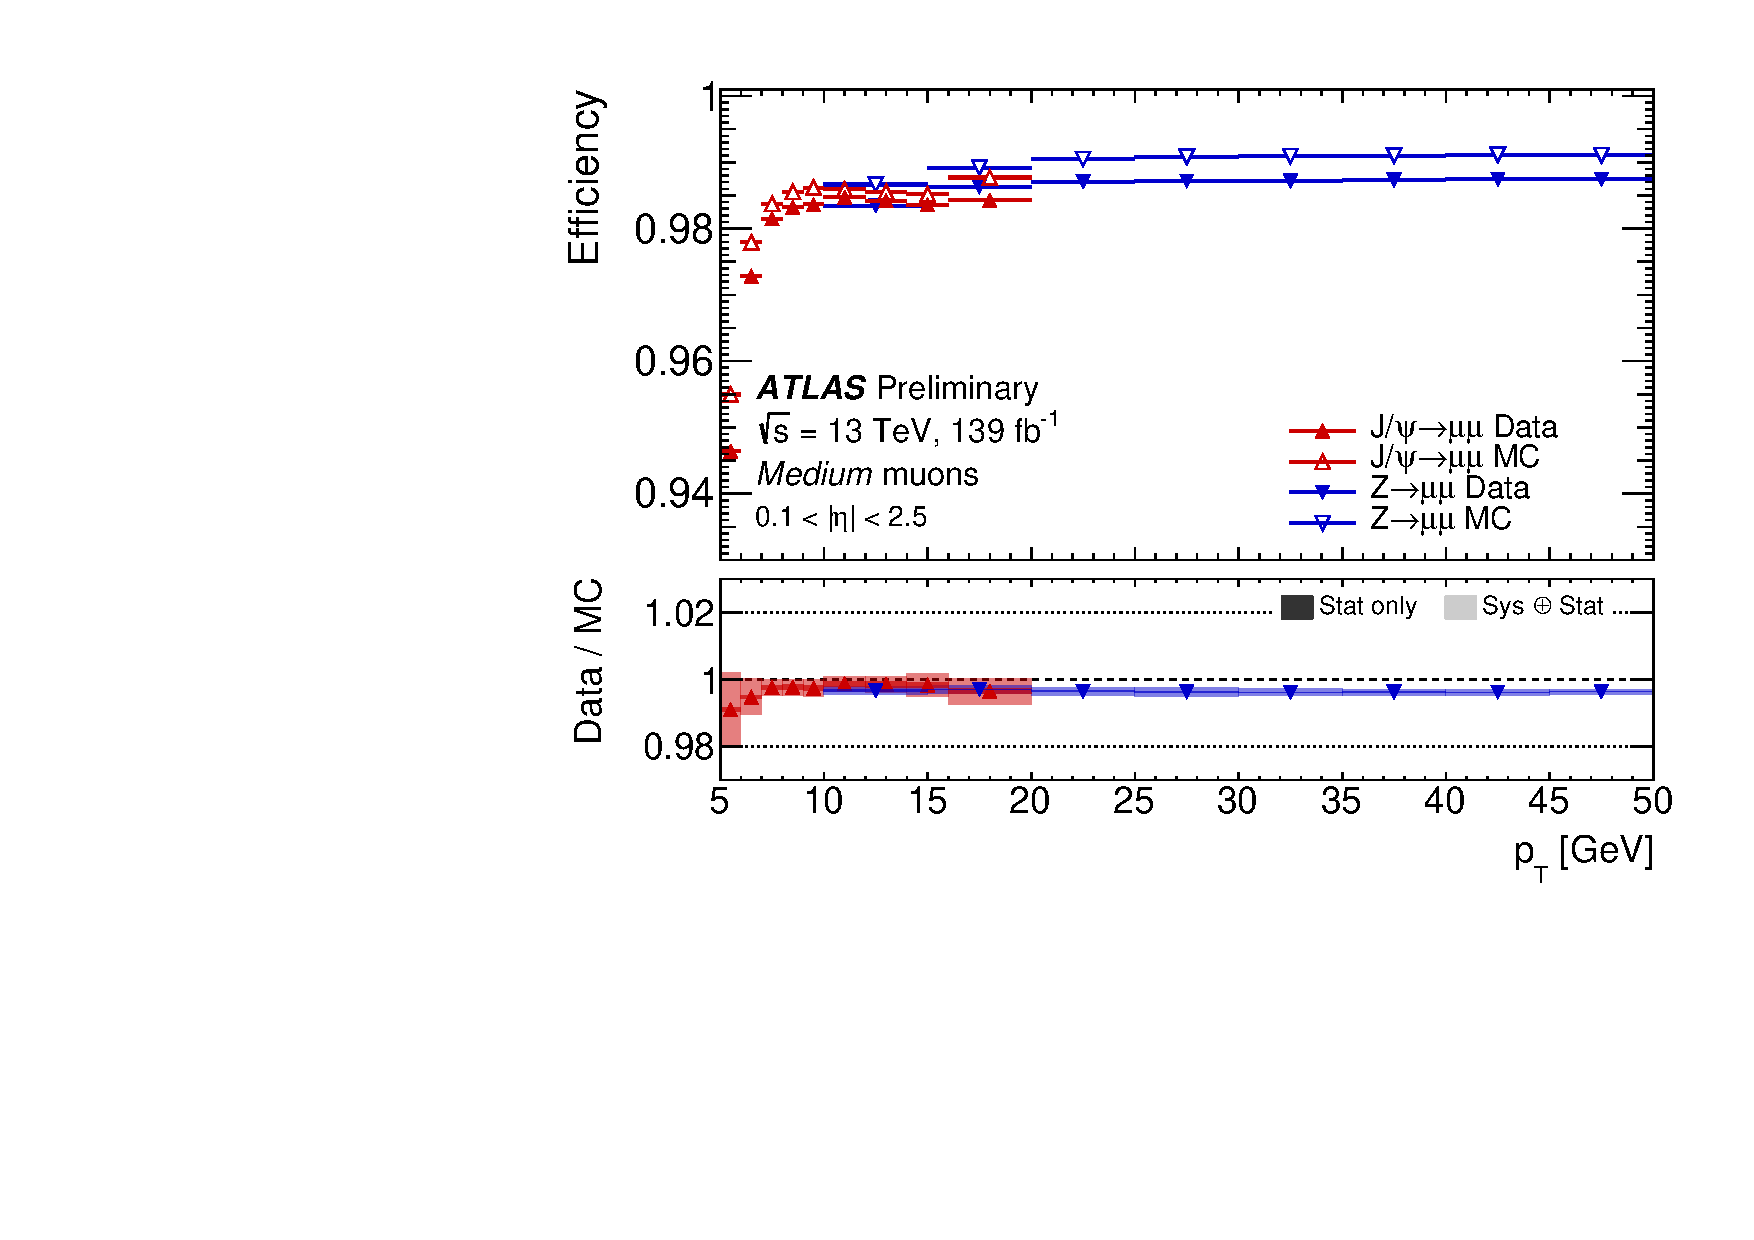
\includegraphics[width=0.95\textwidth]{figures/methods/muon_id_pt.pdf}
      \caption{Muon reconstruction and identification efficiencies in bins of \pt for muons with \(0.1 < \abs{\eta} < 2.5\). The bottom panel shows the ratio of the measured to predicted efficiencies, with statistical and systematic uncertainties~(shaded boxes).}
      \label{fig:methods:event-reconstruction:muons:identification:pt}
    \end{subfigure}
    \\
    \begin{subfigure}{1.\textwidth}
      \centering
      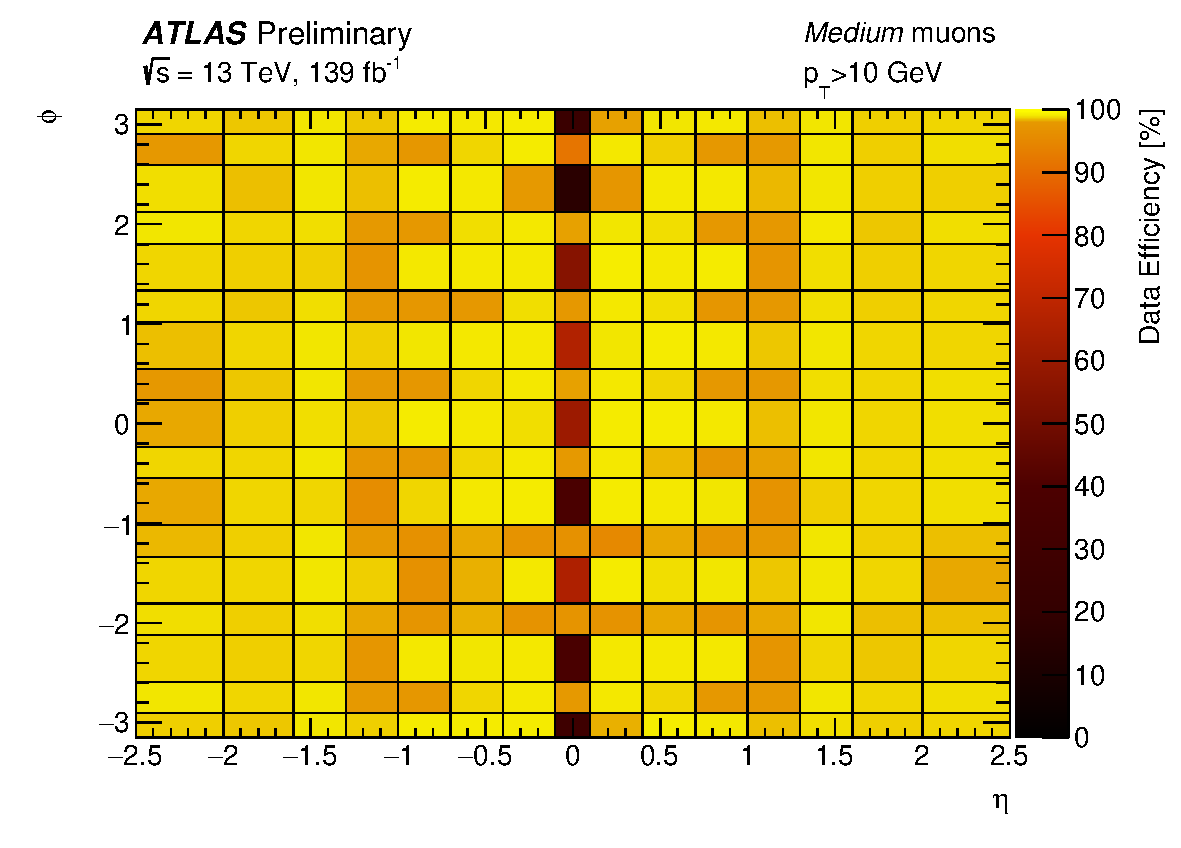
\includegraphics[width=.95\textwidth]{figures/methods/muon_id_eta.pdf}
      \caption{reconstruction and identification efficiencies measured in collision data in bins of \(\eta\)-\(\varphi\) for muons with \(\pt > \SI{10}{\giga\electronvolt}\) as a function of \(\eta\) and \(\varphi\).}
      \label{fig:methods:event-reconstruction:muons:identification:etaphi}
    \end{subfigure}
    \caption{Muon reconstruction and identification efficiencies for \textsc{Medium} muons with \(\pt > \SI{10}{\giga\electronvolt}\). Figures reproduced from Ref.~\cite{ATLAS-CONF-2020-030}.}
    \label{fig:methods:event-reconstruction:muons:identification}
\end{figure}

Additional requirements are imposed on the impact parameters of the muon track to associate the muon candidates with the PV and thereby reject muons originating from cosmic rays, pile-up interactions, or muons originating from secondary hadron decays. The shortest distance from the muon track to the primary vertex in a longitudinal projection is required to satisfy \(\abs{z_{0}} \sin \theta < \SI{0.5}{\milli\meter}\) and the transverse impact parameter significance is required to satisfy \(\abs{d_{0}} / \sigma(d_{0}) < 3\).


\subsubsection{Muon isolation}
Similar to the case of electrons, specific isolation requirements allow for better discrimination between muons from signal processes and background-like objects. Track-based and calorimeter-based isolation variables are employed.
\begin{itemize}
	\item The track isolation variable \(p_{T}^{\text{varcone}, 0.2}\) is defined as the sum of the transverse momenta of all tracks in a cone of variable size \(R = \min \{0.2, \SI{10}{\giga\electronvolt} / \pt\}\) around the direction of the muon with transverse momentum \pt.
	The \(p_{T}^{\text{varcone}, 0.3}\) variable is defined similarly.
	\item The calorimeter \(E_{T}^{\text{cone}, 0.2}\) isolation variable is defined as the sum of the transverse energies of all calorimeter clusters in a cone with fixed size \(R=0.2\) around the muon.
\end{itemize}

Several OPs can be defined using these variables, which either apply a fixed cut on the selected isolation variable or target a specific value of the isolation efficiency in dependence on the muon \pt.

\Cref{fig:methods:event-reconstruction:muons:isolation} shows the muon isolation efficiency for the \textsc{Loose} and \textsc{Tight} fixed cut OPs in bins of \pt.
\begin{figure}[htbp]
    \centering
    \begin{subfigure}{.49\textwidth}
      \centering
      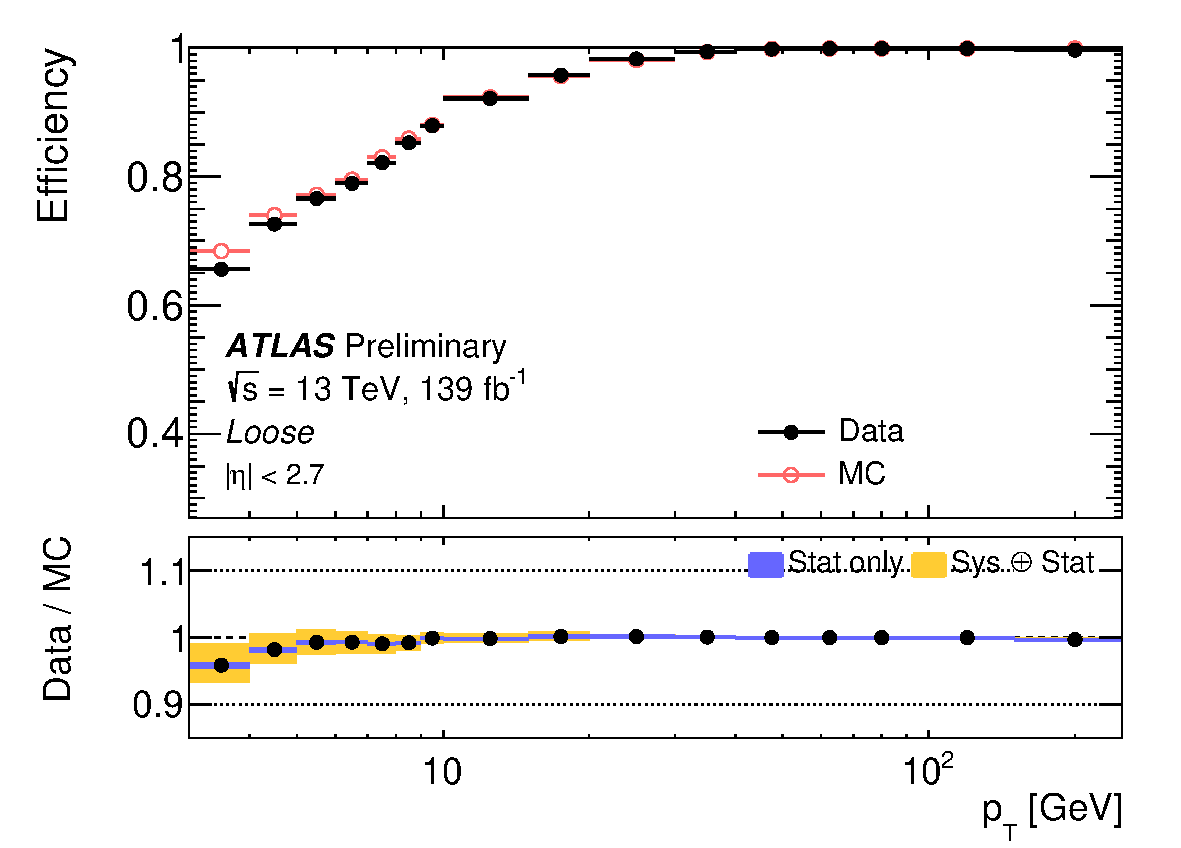
\includegraphics[width=1.\textwidth]{figures/methods/muon_iso_loose.pdf}
      \caption{\textsc{Loose} OP}
      \label{fig:methods:event-reconstruction:muons:isolation:loose}
    \end{subfigure}
    \begin{subfigure}{.49\textwidth}
      \centering
      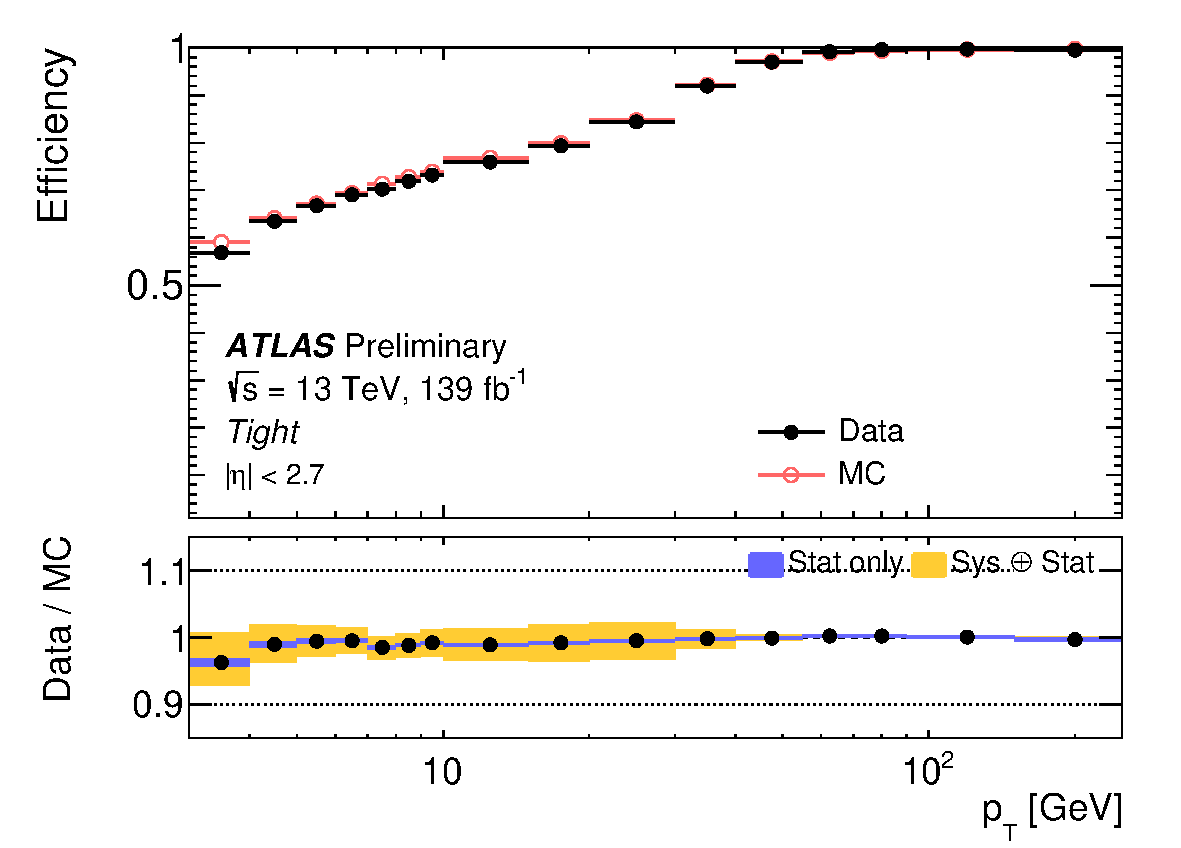
\includegraphics[width=1.\textwidth]{figures/methods/muon_iso_tight.pdf}
      \caption{\textsc{Tight} OP}
      \label{fig:methods:event-reconstruction:muons:isolation:tight}
    \end{subfigure}
    \caption{Muon isolation efficiency in bins of \pt for the \textsc{Loose} and \textsc{Tight} fixed cut OPs. Figures reproduced from Ref.~\cite{ATLAS-CONF-2020-030}.}
    \label{fig:methods:event-reconstruction:muons:isolation}
\end{figure}


\subsection{Jets}
\label{sec:methods:event-reconstruction:jets}
Jets are collimated and localised sprays of particles, which can be reconstructed using jet algorithms (c.f. \Cref{sec:pp:jets}). The \antikt algorithm is used to build jets from topological clusters in the calorimeters, tracks in the ID or stable particles defined by MC event generators. Various radius parameters are used to define in the jet reconstruction, ranging from \(0.2\), \(0.4\), to \(1.0\), including definitions of \pt-dependent radius parameters.
Jets are essential for analyses targeting hadronic final states because they allow associating detector measurements with the parton shower initiated by a single final-state parton.

Jets on detector-level can be built from the energy deposits in the calorimeter, referred to as calorimeter jets or simply jets, or from ID tracks of charged particles, referred to as track jets. While calorimeter jets have a better energy resolution due to the calorimeters also measuring the energy deposits of neutral particles, the track jets have a better spatial resolution due to the intrinsically finer granularity of the ID.
Jets built from stable particles (except muons, neutrinos, and particles from pile-up interactions) in the MC simulation of physics processes are referred to as truth jets. They are used as a reference for the jets reconstructed from detector information in performance studies or early optimisation studies of analyses.

In the following, the reconstruction and calibration of calorimeter jets with small radius parameter, calorimeter jets with large radius parameter, and track jets with fixed and variable radius parameters are described.

\subsubsection{Small-radius calorimeter jets}
\label{sec:methods:event-reconstruction:jets:smallr}
Small-radius calorimeter jets are reconstructed from the topological clusters in the calorimeters calibrated to the EM scale using the \antikt algorithm with a radius parameter \(R=0.4\). The energy scale of the reconstructed small-radius jets is calibrated to the scale particles in MC simulations using a sequence of data- and simulation-based calibrations~\cite{PERF-2016-04,JETM-2018-05}.

The jets produced in the hard-scattering process are expected to originate from the primary vertex. Therefore, the jet direction is recalculated to account for the position of the primary vertex in each event. As a result, the spatial resolution of jets is improved, while keeping the jet energy unchanged.

The sequential calibration scheme, which involves five steps, is illustrated in \Cref{fig:methods:event-reconstruction:jets:smallr:calibration}.

\begin{figure}[htbp]
	\centering
	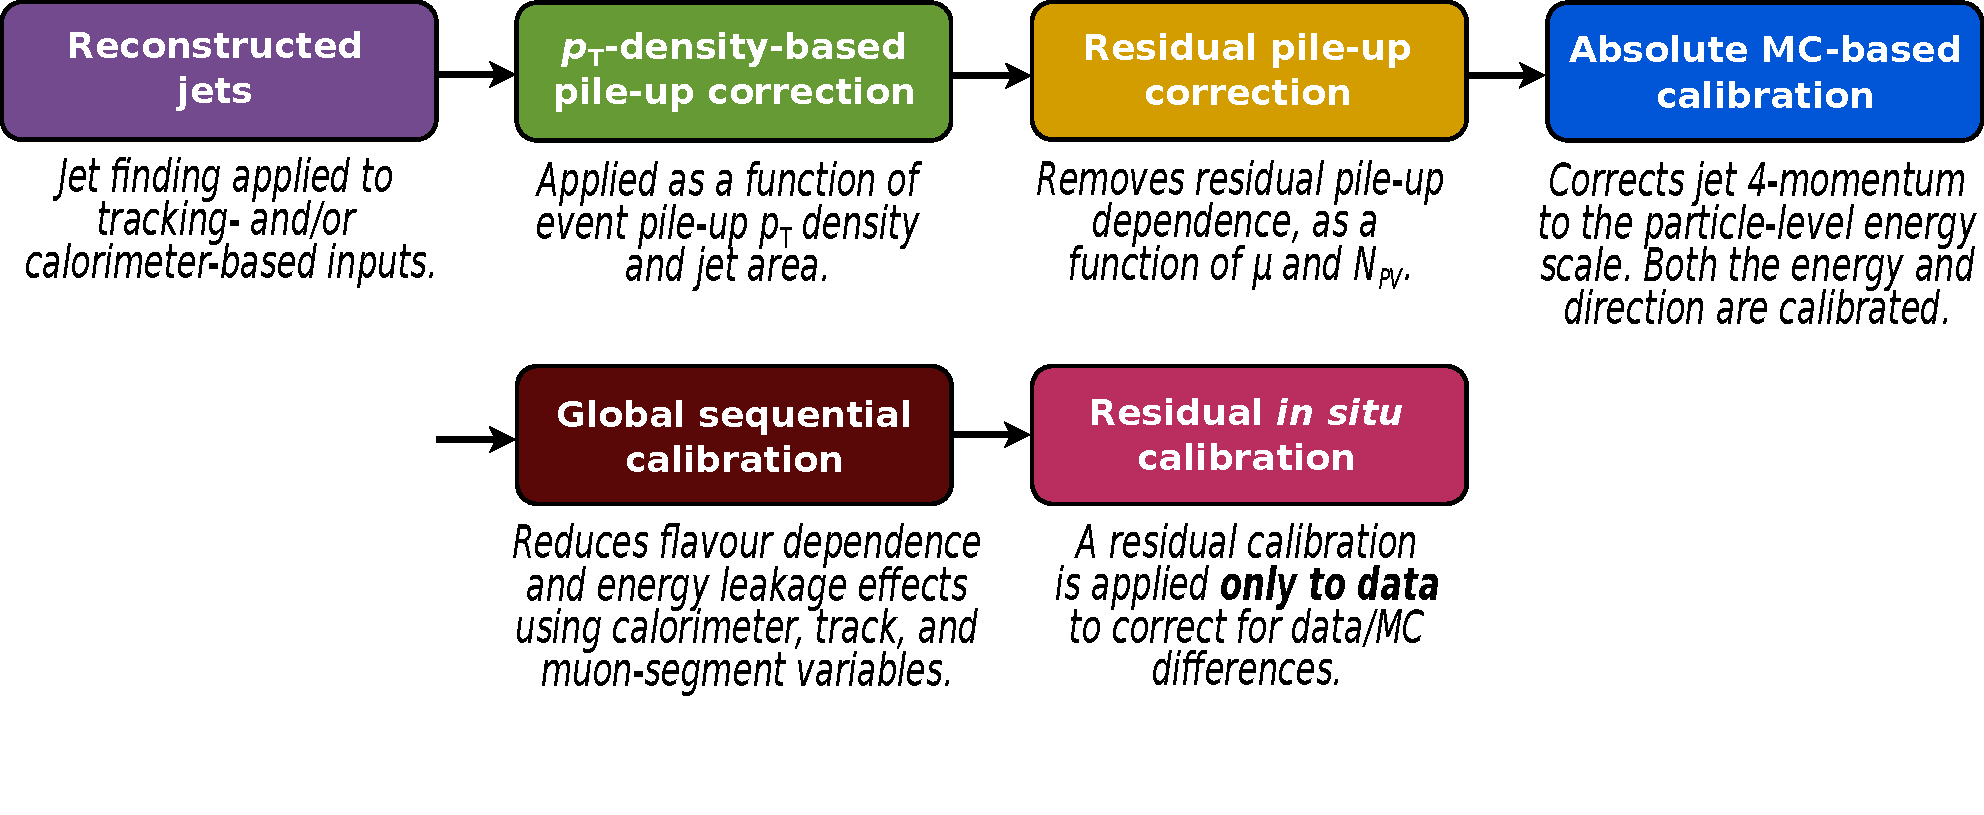
\includegraphics[width=0.95\textwidth]{figures/methods/jet_smallr_calibration.pdf}
	\caption{Stages of jet energy scale calibrations. Each one is applied to the four-momentum of the jet. Figure reproduced from Ref.~\cite{JETM-2018-05}}
	\label{fig:methods:event-reconstruction:jets:smallr:calibration}
\end{figure}

The reconstructed jets first need to be corrected for pile-up by removing the excess energy due to additional \HepProcess{\Pp\Pp} interactions. The pile-up corrections consist of two steps. First, a correction based on the jet area and transverse momentum density of the event is applied. Second, a residual correction derived from MC simulations is applied to remove the remaining dependence on pile-up contributions.
The pile-up corrected jets are calibrated to the particle-level using an MC-based calibration, which corrects their energy and direction. The jet \pt resolution is improved by applying a global sequential calibration. Finally, a residual in-situ calibration is applied to the jets, which corrects for remaining differences between data and simulation.

\begin{enumerate}
	\item \textbf{\pt-density based pile-up correction}. A \pt-density-based subtraction of the event pile-up is performed based on the jet area \(A\) (c.f. ~\Cref{sec:pp:jets}, which is a measure of the susceptibility of the jet to pile-up contributions. The median jet \pt-density \(\rho = \expval{\pt / A}\) is used to estimate the median pile-up contribution in jets. It is calculated from jets in the central lower-occupancy regions \(\abs{\eta} < 2.0\) of the calorimeter, which are reconstructed from topological clusters using the \(k_{\text{T}}\) algorithm with \(R=0.4\) in the rapidity-\(\varphi\) plane.

	\item \textbf{Residual pile-up correction}. After the \pt-density-based correction, some residual dependence on the pile-up activity remains. It is estimated in MC simulations by geometrically matching the reconstructed jets to truth jets within \(\Delta R < 0.3\) and parametrising the difference between the reconstructed jet \(\pt^{\text{reco}}\) and the corresponding truth jet \(\pt^{\text{truth}}\) as a function of the number of reconstructed primary vertices \(N_{\text{PV}}\) and the mean number of interactions per bunch crossing \(\mu\). The former number is a measure of the in-time pile-up, while the latter is a measure for out-of-time pile-up. The residual momentum dependence on \(N_{\text{PV}}\) and \(\mu\) is parametrised as linear functions.

	The jet \pt after both pile-up corrections is
	\(\pt^{\text{PU corr}} = \pt^{\text{reco}} - \rho \times A - \alpha \times (N_{\text{PV}} - 1) - \beta \times \mu\), where \(\pt^{\text{reco}}\) denotes the reconstructed jet \pt before pile-up corrections and \(\alpha, \beta\) are coefficients defined in \(\pt\) and \(\eta\) of the truth jet.

	The dependence of the jet \pt on \(N_{\text{PV}}\) and \(\mu\) is shown in \Cref{fig:methods:event-reconstruction:jets:smallr:pileup}.
\end{enumerate}
\begin{figure}[htbp]
    \centering
    \begin{subfigure}{.49\textwidth}
      \centering
      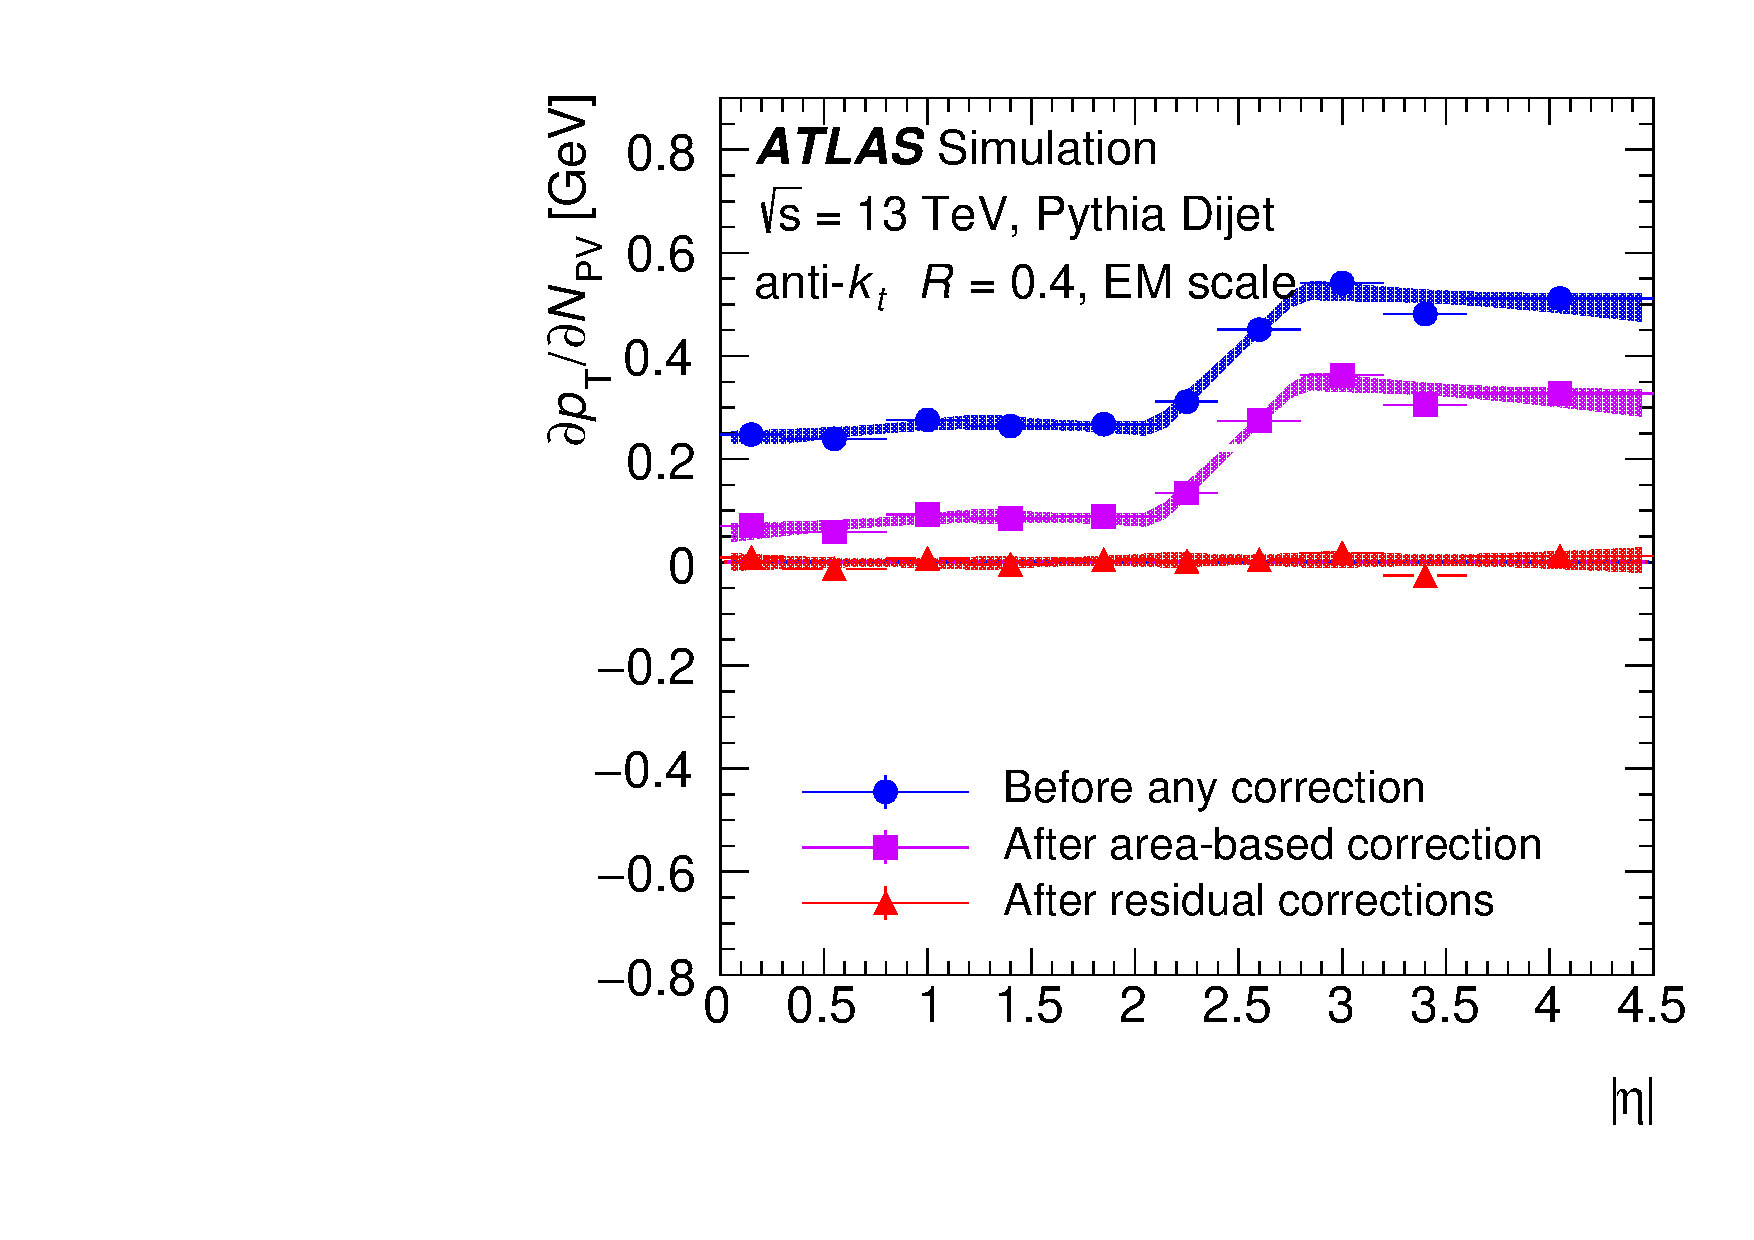
\includegraphics[width=1.\textwidth]{figures/methods/jet_pu-npv.pdf}
      \caption{Dependence of jet \pt on \(N_{\text{PV}}\), averaged over \(\mu\).}
      \label{fig:methods:event-reconstruction:jets:pileup-npv}
    \end{subfigure}
    \begin{subfigure}{.49\textwidth}
      \centering
      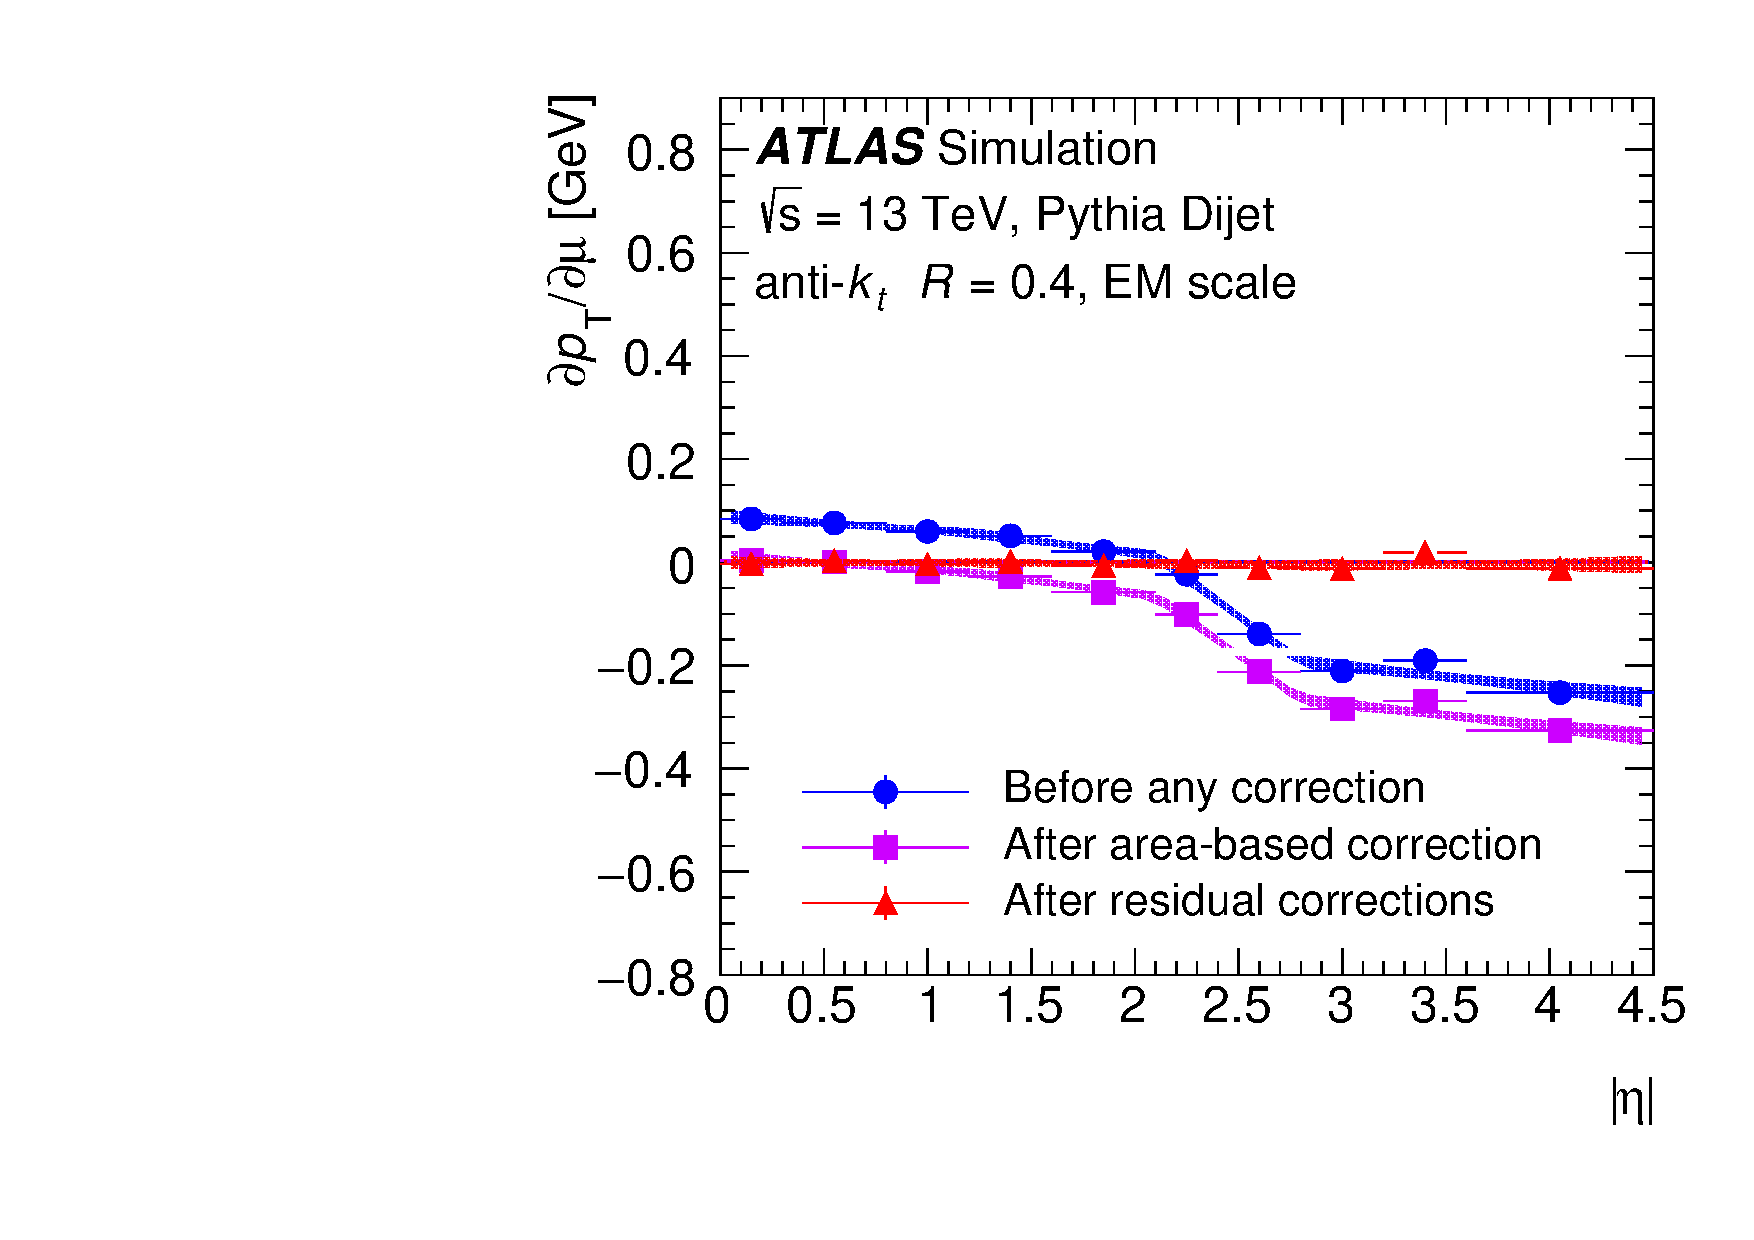
\includegraphics[width=1.\textwidth]{figures/methods/jet_pu-mu.pdf}
      \caption{Dependence of jet \pt on \(\mu\), averaged over \(N_{\text{PV}}\).}
      \label{fig:methods:event-reconstruction:jets:pileup-mu}
    \end{subfigure}
    \caption{Dependence of jet \pt on in-time pile-up (left) and out-of-time pile-up (right) as a function of \(\abs{\eta}\) for truth jet \(\pt = \SI{25}{\giga\electronvolt}\). Figures reproduced from Ref.~\cite{PERF-2016-04}.}
    \label{fig:methods:event-reconstruction:jets:smallr:pileup}
\end{figure}
\begin{enumerate}
	\setcounter{enumi}{2}
	\item \textbf{Absolute MC-based calibration}. The absolute jet energy scale (JES) and \(\eta\)-calibrations correct the reconstructed and pile-up corrected jet four momenta to the energy scale of final-state particles by accounting for non-compensating calorimeter response, energy losses in the dead material, out-of-cone effects, and biases in the jet \(\eta\)-reconstruction. Both JES and \(\eta\) calibration are parametrised in the reconstructed jet energy \(E^{\text{reco}}\) and the pseudorapidity in the detector coordinate frame \(\eta_{\text{det}}\).

	The JES calibration applies a correction, which is taken as the inverse of the average jet energy response \(\mathcal{R}\). The jet energy response \(\mathcal{R}\) is defined as the mean of a Gaussian fit to the core of the \(E^{\text{reco}} / E^{\text{truth}}\) distribution. The average jet energy response for jets with different \(E^{\text{truth}}\) as a function of \(\eta_{\text{det}}\) is shown in \Cref{fig:methods:event-reconstruction:jets:smallr:response-average}.

	The \(\eta\) calibration corrects for biases in the reconstructed jet \(\eta\), which are defined as deviations from zero in the signed difference between the reconstructed pseudorapidity \(\eta^{\text{reco}}\) and the truth pseudorapidity \(\eta^{\text{truth}}\). \Cref{fig:methods:event-reconstruction:jets:smallr:response-eta} shows the signed difference as a function of \(\eta_{\text{det}}\).

	These calibrations only change the jet \pt and \(\eta\), not the full four-momentum. Jets calibrated with the full JES and \(\eta\) calibration, are considered to be at the EM+JES scale.
\end{enumerate}
\begin{figure}[htbp]
    \centering
    \begin{subfigure}{.49\textwidth}
      \centering
      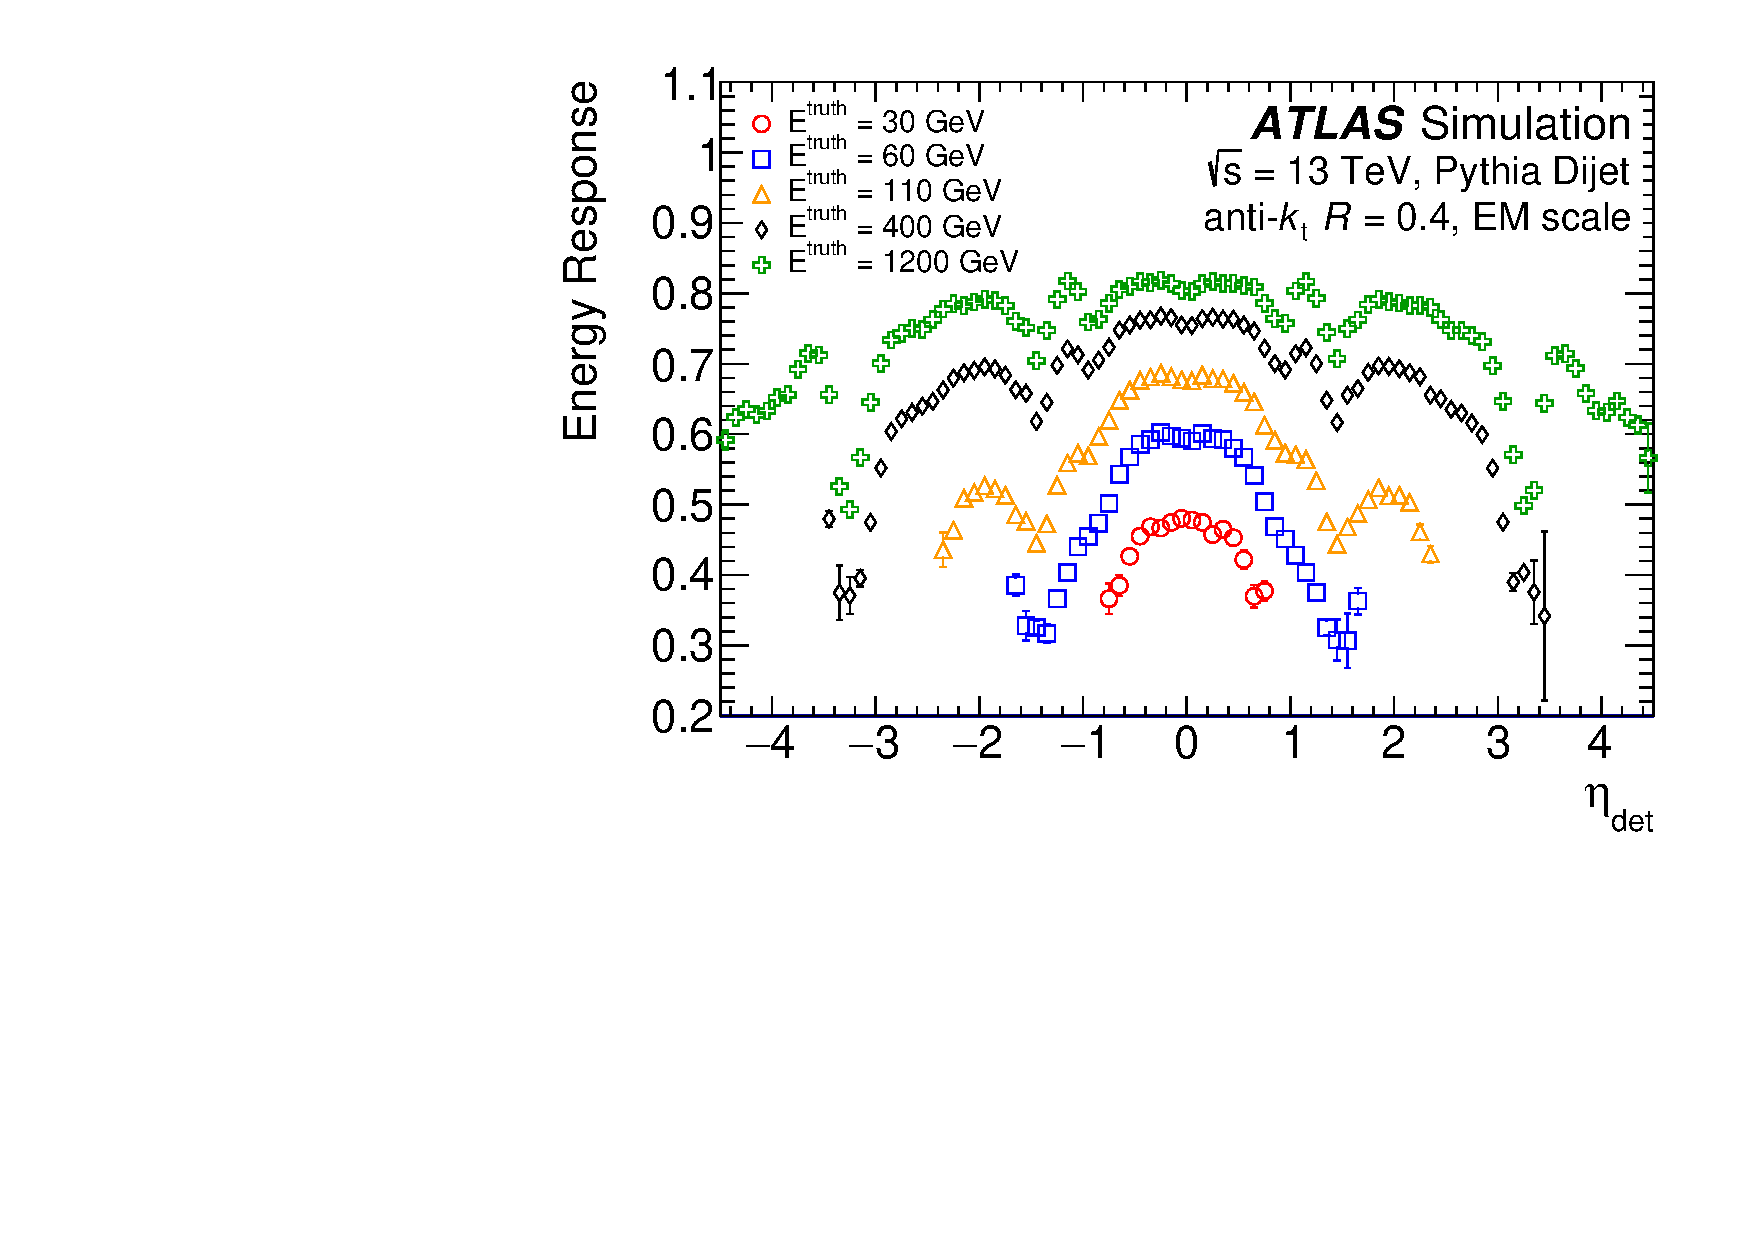
\includegraphics[width=1.\textwidth]{figures/methods/jet_response-average.pdf}
      \caption{Average jet energy response.}
      \label{fig:methods:event-reconstruction:jets:smallr:response-average}
    \end{subfigure}
    \begin{subfigure}{.49\textwidth}
      \centering
      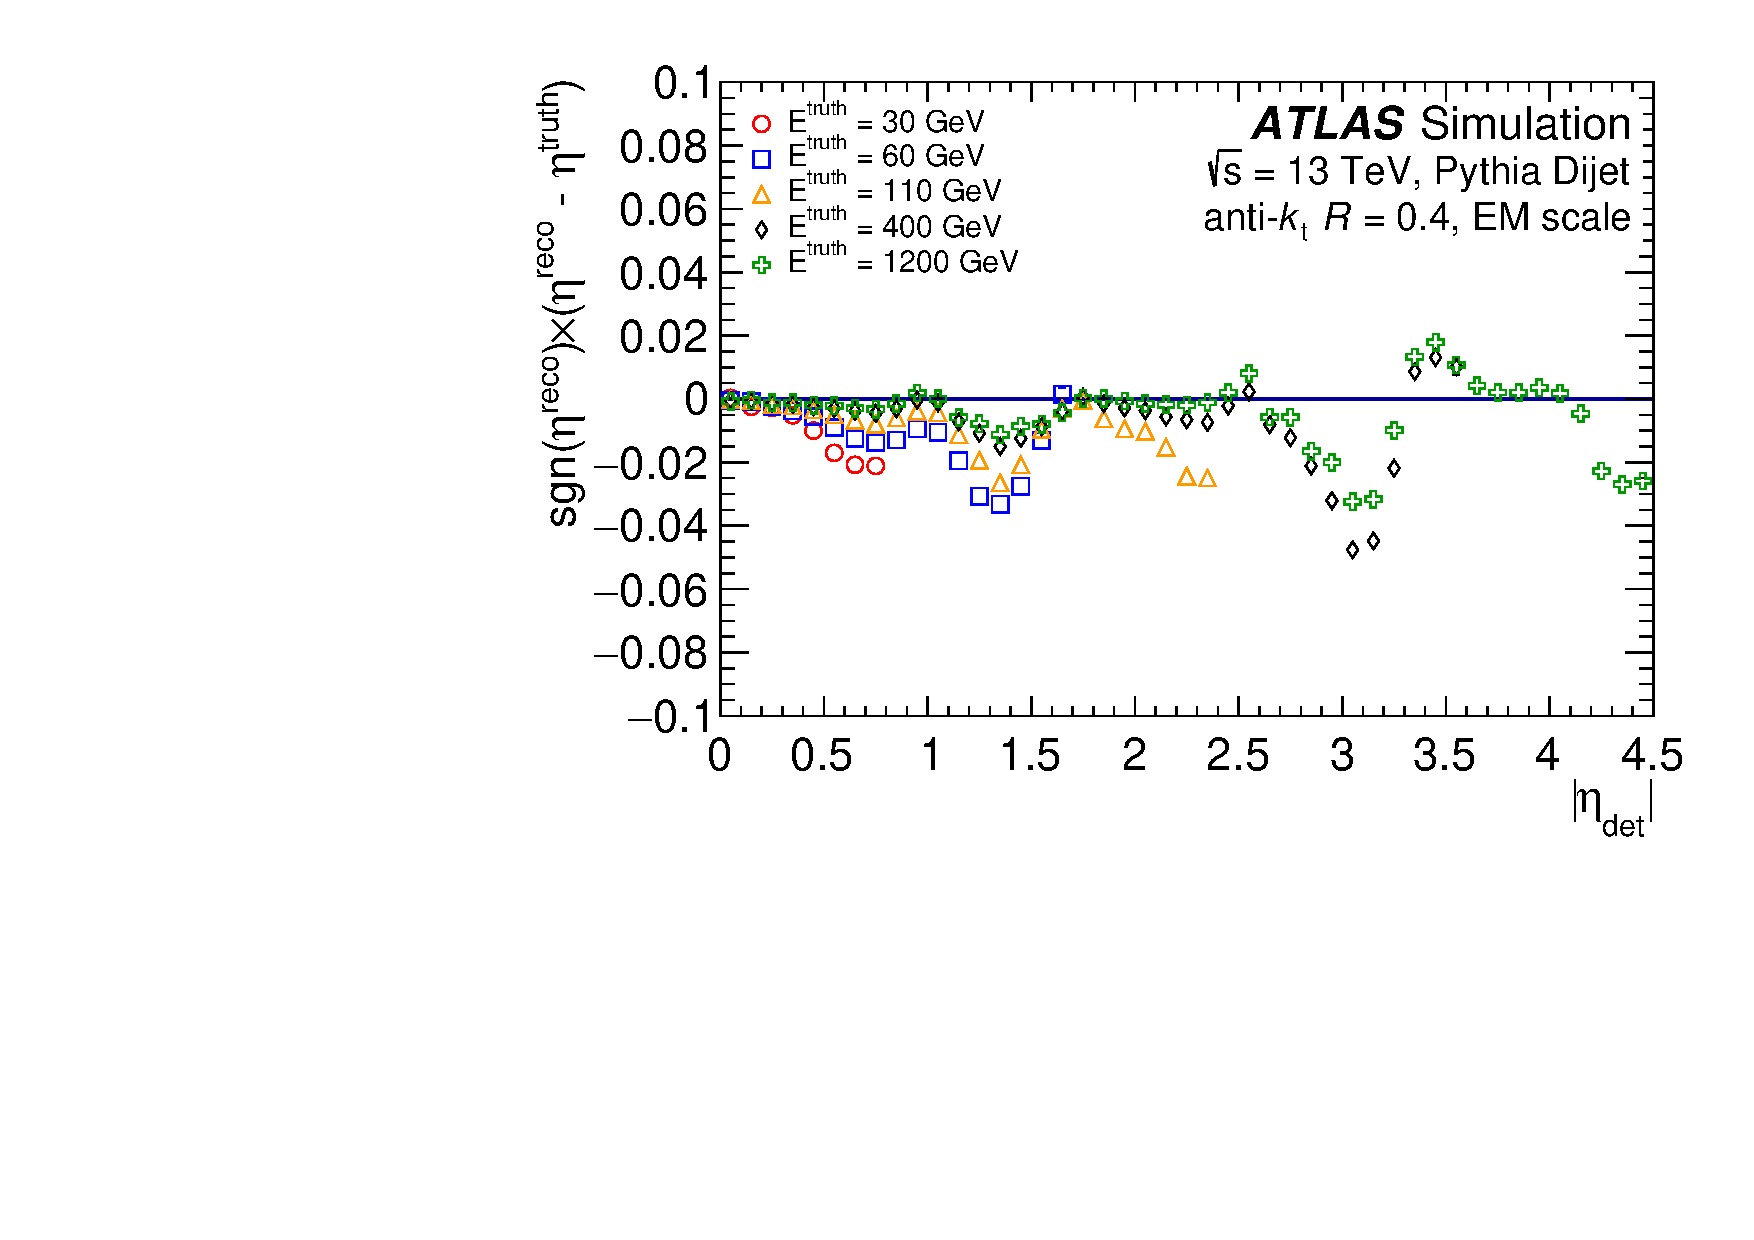
\includegraphics[width=1.\textwidth]{figures/methods/jet_response-eta.pdf}
      \caption{Signed difference between reconstructed and truth \(\eta\) as a function of \(\eta_{\text{det}}\).}
      \label{fig:methods:event-reconstruction:jets:smallr:response-eta}
    \end{subfigure}
    \caption{The average jet energy response (left) and the signed difference between the truth and the reconstructed jet pseudorapidity (right) as functions of \(\eta_{\text{det}}\) for jets with truth energy of \num{30}, \num{60}, \num{110}, \num{400}, and \SI{1200}{\giga\electronvolt}. Figures reproduced from Ref.~\cite{PERF-2016-04}.}
    \label{fig:methods:event-reconstruction:jets:smallr:response}
\end{figure}
\begin{enumerate}
	\setcounter{enumi}{3}
	\item \textbf{Global Sequential Calibration}. The residual dependencies of jets at the EM+JES scale on features of the jet due to fluctuations in the jet particle composition and the distribution of energy within the jet are taken into account by a Global Sequential Calibration (GSC). The GSC is a series of multiplicative corrections, which are based on five jet observables, such as jet topological energy distributions or number of tracks associated with the jets. For each jet observable, an independent correction of the jet four-momentum is derived as a function jet \pt, jet energy, and \(\abs{\eta_{\text{det}}}\).

	\item \textbf{Residual in-situ calibration}. The final in-situ calibration step accounts for differences between the jet response in data and simulation by measuring the jet response in data and MC simulation separately and applying the ratio as an additional correction in data only. There are three in-situ calibrations, which are obtained from dedicated measurements involving well-calibrated reference objects. First, the jets in the forward region of the detector (\(0.8 < \abs{\eta_{\text{det}}} < 4.5\)) receive an additional correction, which brings them to the same energy scale as the jets in the central region with \( \abs{\eta_{\text{det}}} < 0.8\). Second, the jet \pt is calibrated in \HepProcess{\PZ(\Pl\Pl) + \text{jets}} and \HepProcess{\Pgamma + \text{jets}} events by balancing the hadronic recoil against a well-calibrated \PZ boson or photon. Third, single high-\pt jets are calibrated in multijet events by balancing the momentum against a system of several well-calibrated low-\pt jets. The calibration factors of the three steps are combined to a final in-situ calibration map, as shown in \Cref{fig:methods:event-reconstruction:jets:smallr:insitu}.
\end{enumerate}
\begin{figure}[htbp]
    \centering
    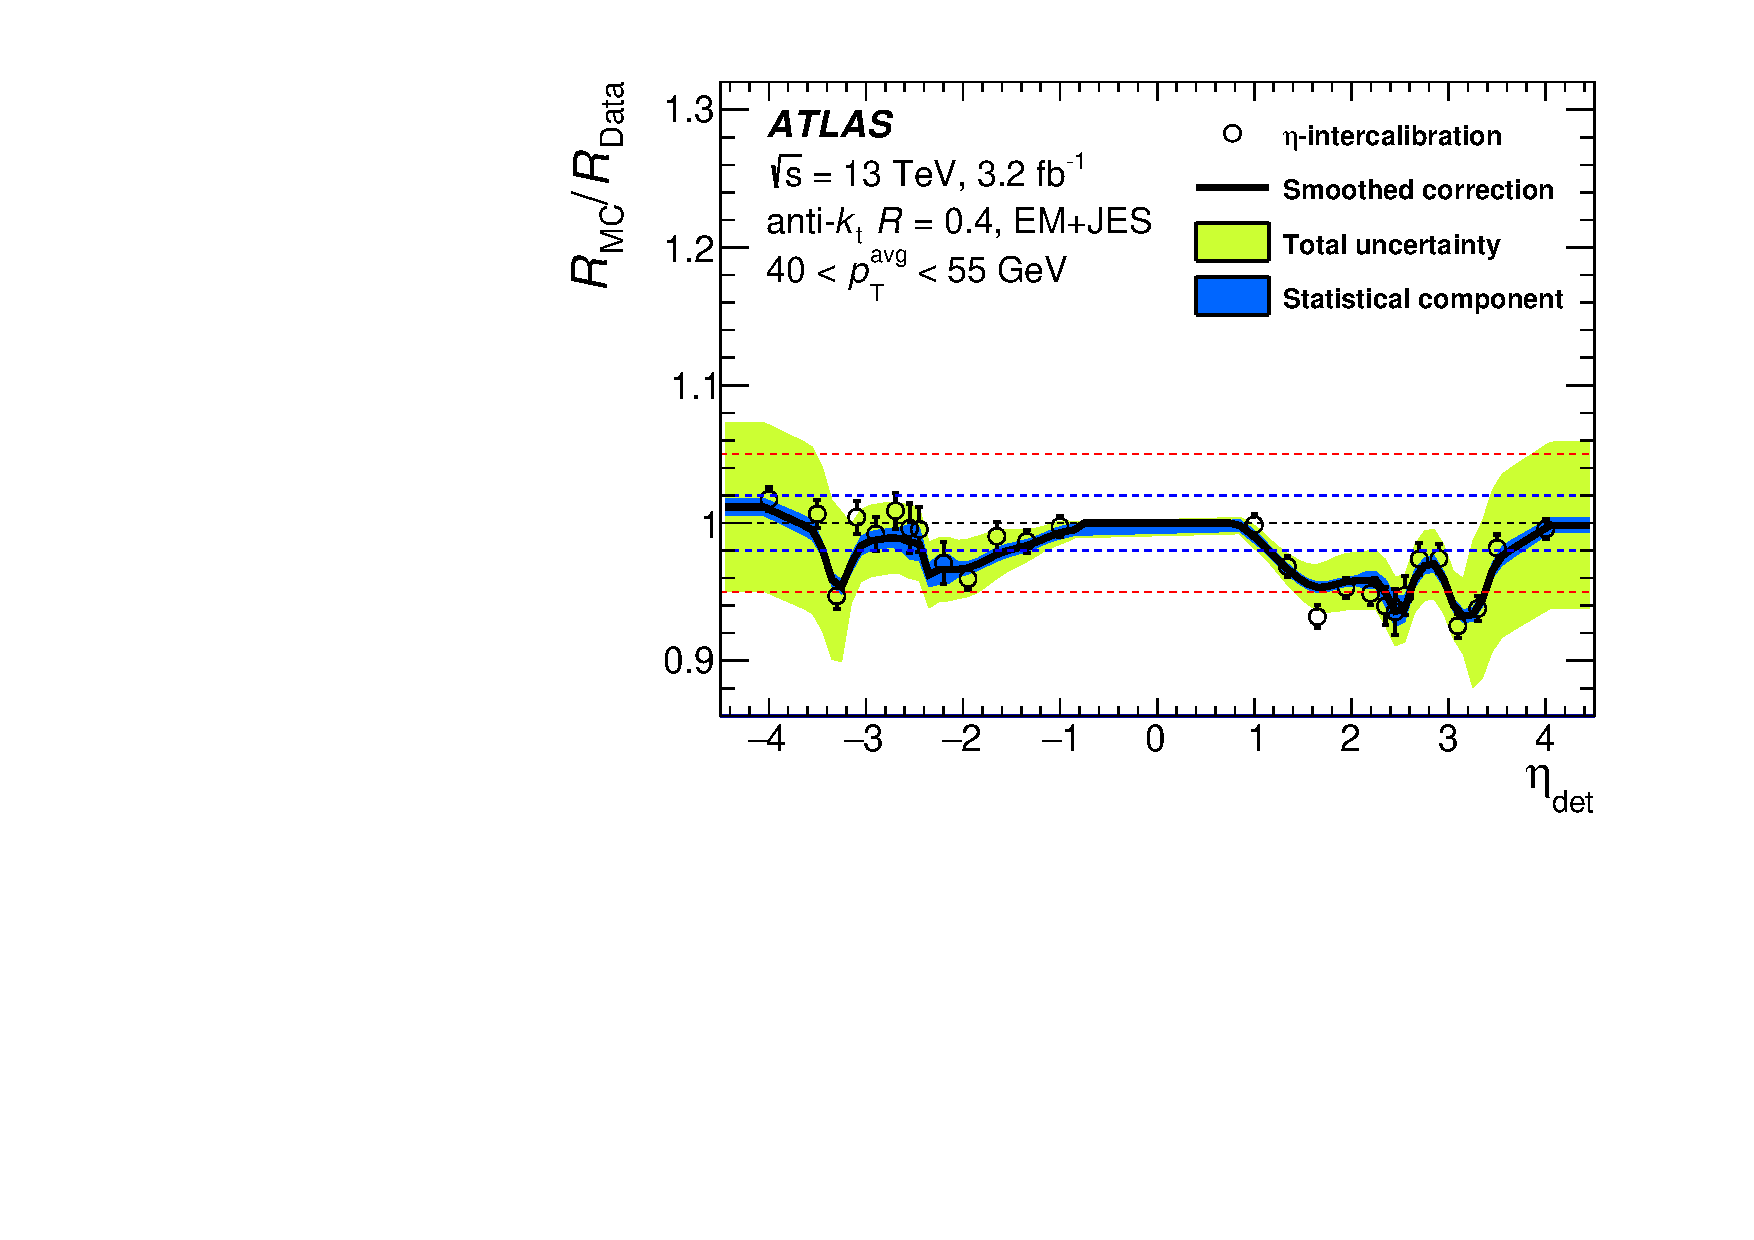
\includegraphics[width=.95\textwidth]{figures/methods/jet_insitu.pdf}
    \caption{Binned ratio (open circles) of the jet response in simulated events to that in data as a function of \(\eta_{\text{det}}\) for jets at the EM+JES and GSC scale with \(\SI{40}{\giga\electronvolt} < \pt^{\text{avg}} < \SI{55}{\giga\electronvolt}\). The smoothed correction (black line) with corresponding statistical (dark blue) and total (light green) uncertainty bands is overlaid, together with horizontal dotted lines to guide the eye. Figure reproduced from Ref.~\cite{PERF-2016-04}.}
    \label{fig:methods:event-reconstruction:jets:smallr:insitu}
\end{figure}

The JES calibration is accompanied by systematic uncertainties, which are defined using more than \num{90} components. As most of these uncertainties are of minor importance for most physics analyses, reduced sets of JES uncertainties are available, which combine groups of uncertainties and thereby reduce the complexity of statistical models.

In addition to the central value of the JES and the associated calibration uncertainties, the jet energy resolution (JER) needs to be determined~\cite{PERF-2014-02}. It can be parametrised by
\begin{align}
    \frac{\pt}{\sigma(\pt)} = \frac{\mathcal{N}}{\pt} \oplus \frac{\mathcal{S}}{\sqrt{\pt}} \oplus \mathcal{C},
\end{align}
where \(\mathcal{N}\) accounts for the effect of electronic and pile-up noise, \(\mathcal{S}\) denotes the stochastic term arising from the sampling nature of the calorimeters, and \(\mathcal{C}\) denotes the constant term. All terms are added in quadrature.

The JER is measured using the in-situ techniques described above, with the exception that the observable of interest is not the mean of the jet response  \(\mathcal{R}\) but its width \(\sigma(\mathcal{R})\).


\subsubsection{Identification of \bjets}
\label{sec:methods:event-reconstruction:jets:btagging}
The identification of \bjets --- jets originating from the fragmentation of \bquarks --- is an essential experimental technique to identify processes of interest even in the presence of large background contributions~\cite{ATL-PHYS-PUB-2017-013,FTAG-2018-01}.

The characteristic signature of \bjets manifests as at least one displaced decay vertex with respect to the primary vertex because of the relatively long lifetime of \PB-mesons of roughly \SI{1.5}{\pico\second}, which corresponds to a proper decay length of \SI{450}{\micro\meter}.

The identification of \bjets consists of two steps. First, various low-level algorithms process features of ID tracks and estimate their association with displaced vertices. Second, the output of these algorithms is processed by multivariate (MVA) classifiers to provide a powerful discriminant for identifying \bjets. This procedure is commonly referred to as \btagging.

The low-level \btagging algorithms include impact parameter based algorithms (IP2D and IP3D)~\cite{ATL-PHYS-PUB-2017-013}, the secondary vertex finder algorithm (SV1)~\cite{ATL-PHYS-PUB-2017-011}, and the topological multi-vertex algorithm (JetFitter)~\cite{ATL-PHYS-PUB-2018-025}. The algorithms are briefly introduced below.
\begin{itemize}
	\item The \textbf{IP2D and IP3D algorithms} are based on exploiting the large impact parameters of the tracks originating from \PB-hadron decays. While the IP2D algorithm constructs a discriminating variable using only the signed transverse impact parameter significance of tracks, the IP3D algorithm considers both the transverse and longitudinal impact parameter significances \(d_{0} / \sigma(d_{0})\) and \(\sin \theta z_{0} / \sigma(\sin \theta z_{0})\). Based on these discriminating variables and reference distributions from MC simulation, likelihood ratio discriminants are calculated for \bjet, charm jet (\cjet) and light-flavour jet identification.

	\item The \textbf{SV1 algorithm} reconstructs the single displaced vertex inside the jet which corresponds to the \PB-hadron decay using selected tracks, which have to satisfy a set of quality requirements. Likelihood ratio discriminants are constructed from vertex variables, such as the vertex mass, and the number of two-track vertices.

	\item The \textbf{JetFitter algorithm} is designed to reconstruct the full \PB-hadron decay chain, exploiting the topological features of heavy-flavour decays inside the jet. The algorithm is based on a modified Kalman filter, which is used to find a common line on which the primary, bottom and charm vertices lie, approximating the b-hadron flight path as well as the vertex positions. Likelihood ratio discriminants are constructed from the displaced vertex variables.
\end{itemize}

The commonly used high-level \btagging algorithm is the MV2 Boosted Decision Tree (BDT)~\cite{ATL-PHYS-PUB-2017-013}, which combines the outputs of the low-level \btagging algorithms with kinematic properties \pt and \(\eta\) of the jets using MVA techniques. The MV2 algorithm is trained on a mixed sample of simulated \ttbar and \PZprime events, whose background composition is adjusted to \SI{7}{\percent} \cjets and \SI{93}{\percent} light-flavour jets.

The \btagging performance is evaluated using a sample of \ttbar events. Several \btagging single-cut OPs are defined, which are based on a fixed cut on the \btagging algorithm discriminant distribution and correspond to a specific \btagging efficiency. The searches for dark matter presented in this dissertation use OPs corresponding to \SI{70}{\percent} and \SI{77}{\percent} \btagging efficiency. \Cref{fig:methods:event-reconstruction:jets:btagging:mv2} shows the distribution of the MV2 output discriminant, with the selections corresponding to \SI{70}{\percent} and \SI{77}{\percent} efficiency indicated.

\begin{figure}[htbp]
    \centering
    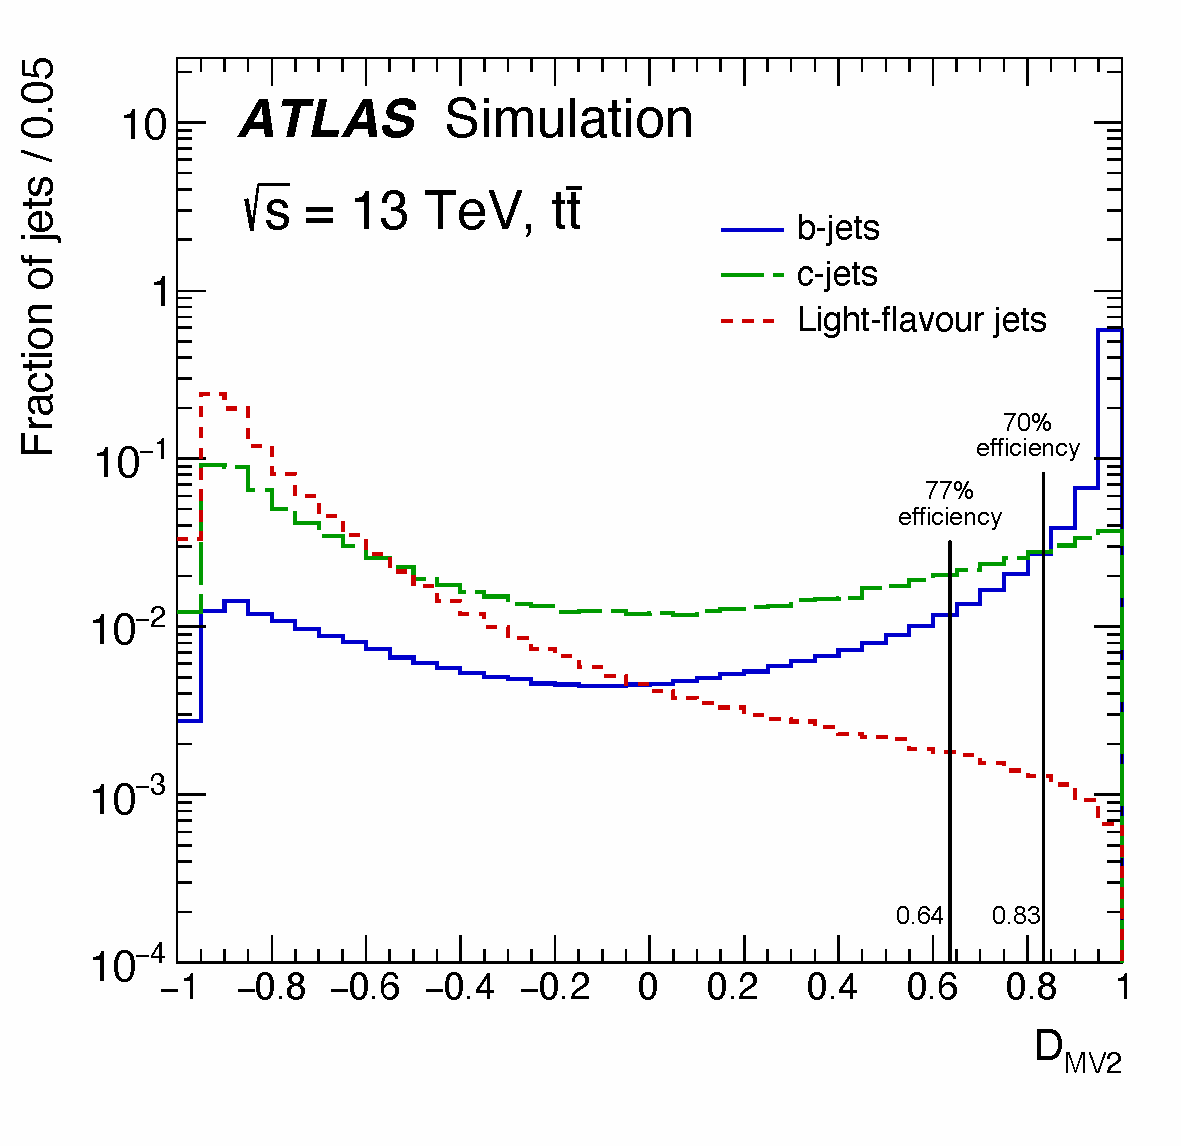
\includegraphics[width=.8\textwidth]{figures/methods/btagging_mv2.pdf}
    \caption{Distribution of the output discriminant of the MV2 \btagging algorithm for \bjets~(blue), \cjets~(green) and light-flavour jets~(red) in a sample of MC simulated \ttbar events. Figure adapted from Ref.~\cite{FTAG-2018-01}.}
    \label{fig:methods:event-reconstruction:jets:btagging:mv2}
\end{figure}

The corresponding rejection factors for \cjets and light-flavour jets at the \SI{77}{\percent} (\SI{70}{\percent}) fixed-cut efficiency selection are approximately \num{5} and \num{110} (\num{9} and \num{300}), respectively.

The \btagging efficiency, as well as the misidentification rates of \cjets and light-flavour jets, are compared between data and simulations. Corrections in the form of scale factors are applied to simulated events to account for discrepancies between data and simulations due to imperfections in the modelling of physics processes or the detector response.

\Cref{fig:methods:event-reconstruction:jets:btagging:corrections} shows the measured \btagging efficiency in dependence of the jet \pt and the scale factors, which are applied to simulated events. The scale factors have values close to unity and are approximately constant throughout the entire \pt range.

\begin{figure}[htbp]
    \centering
    \begin{subfigure}{.49\textwidth}
      \centering
      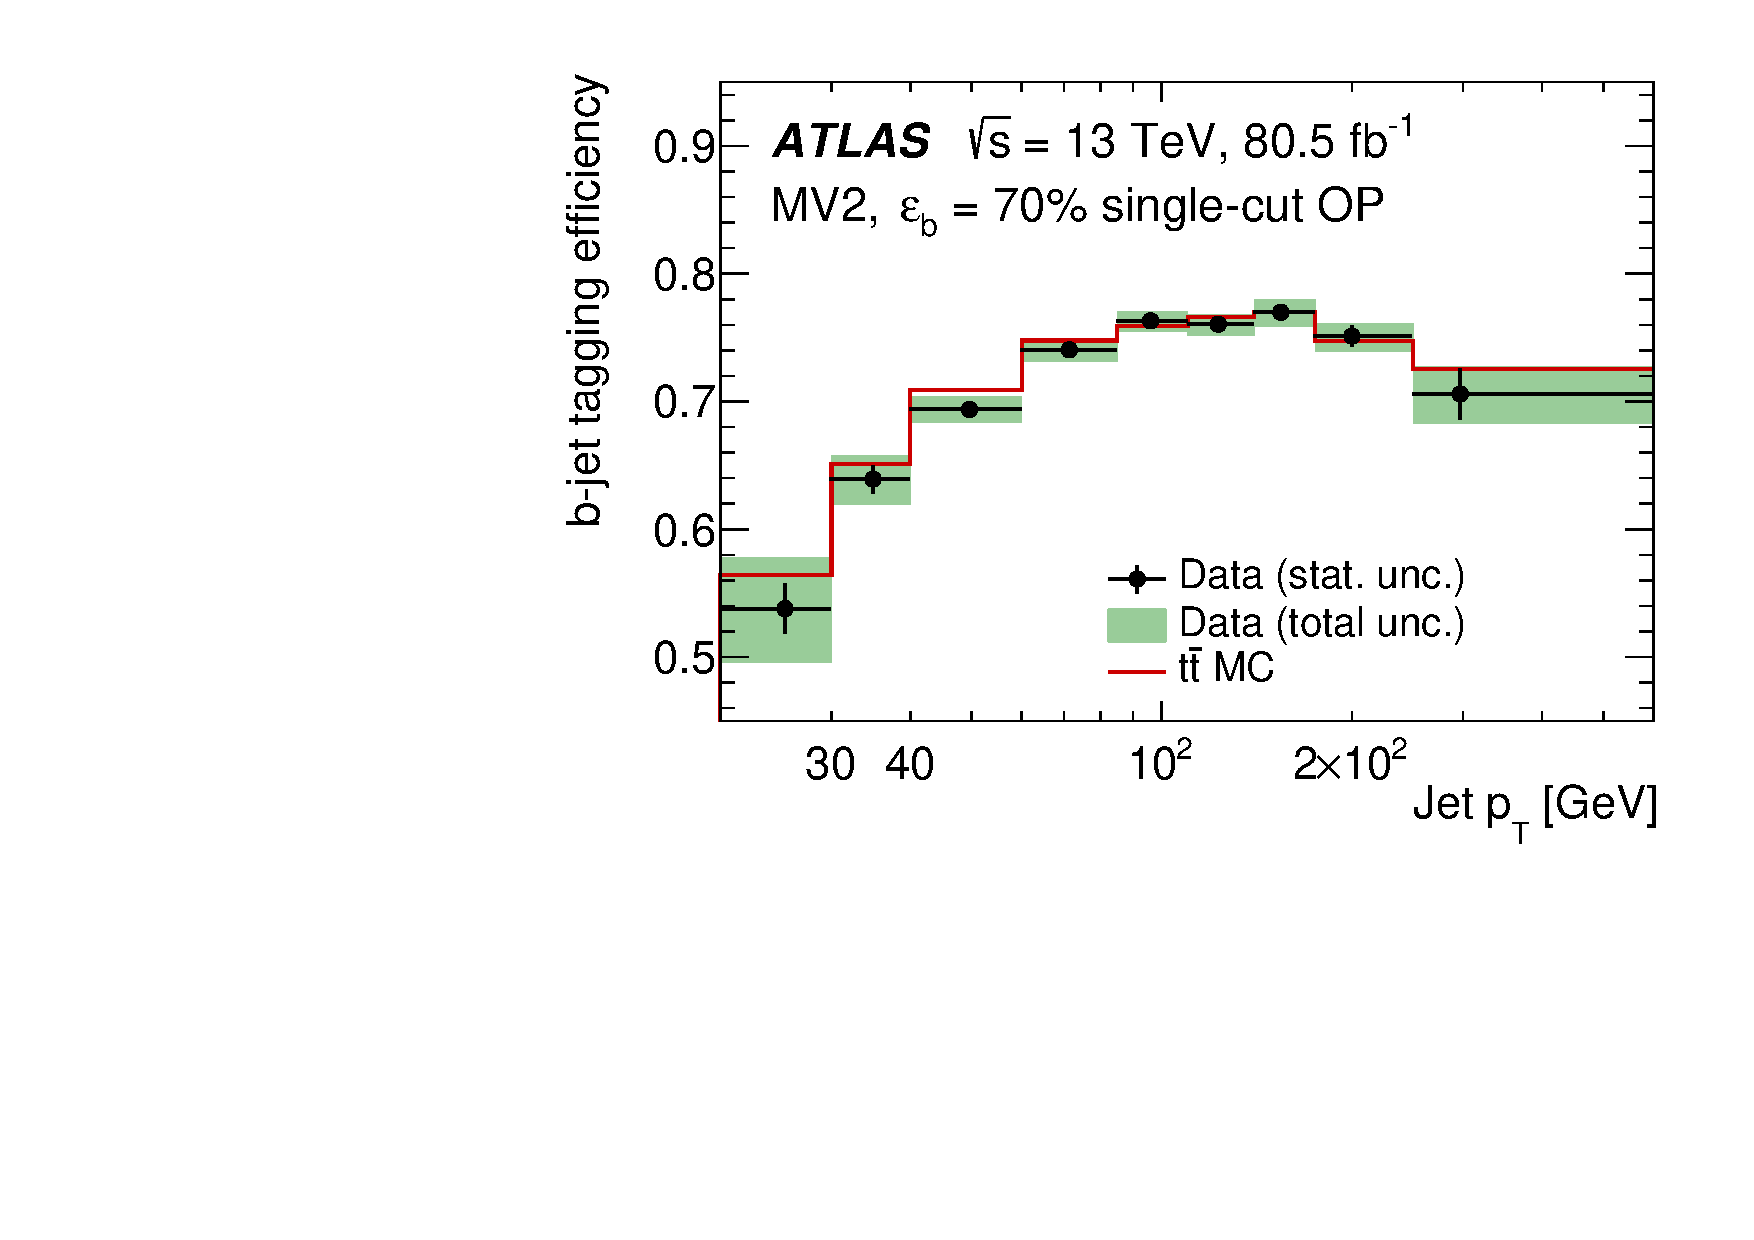
\includegraphics[width=1.\textwidth]{figures/methods/btagging_efficiency70.pdf}
      \caption{\btagging efficiency}
      \label{fig:methods:event-reconstruction:jets:btagging:corrections:efficiency}
    \end{subfigure}
    \begin{subfigure}{.49\textwidth}
      \centering
      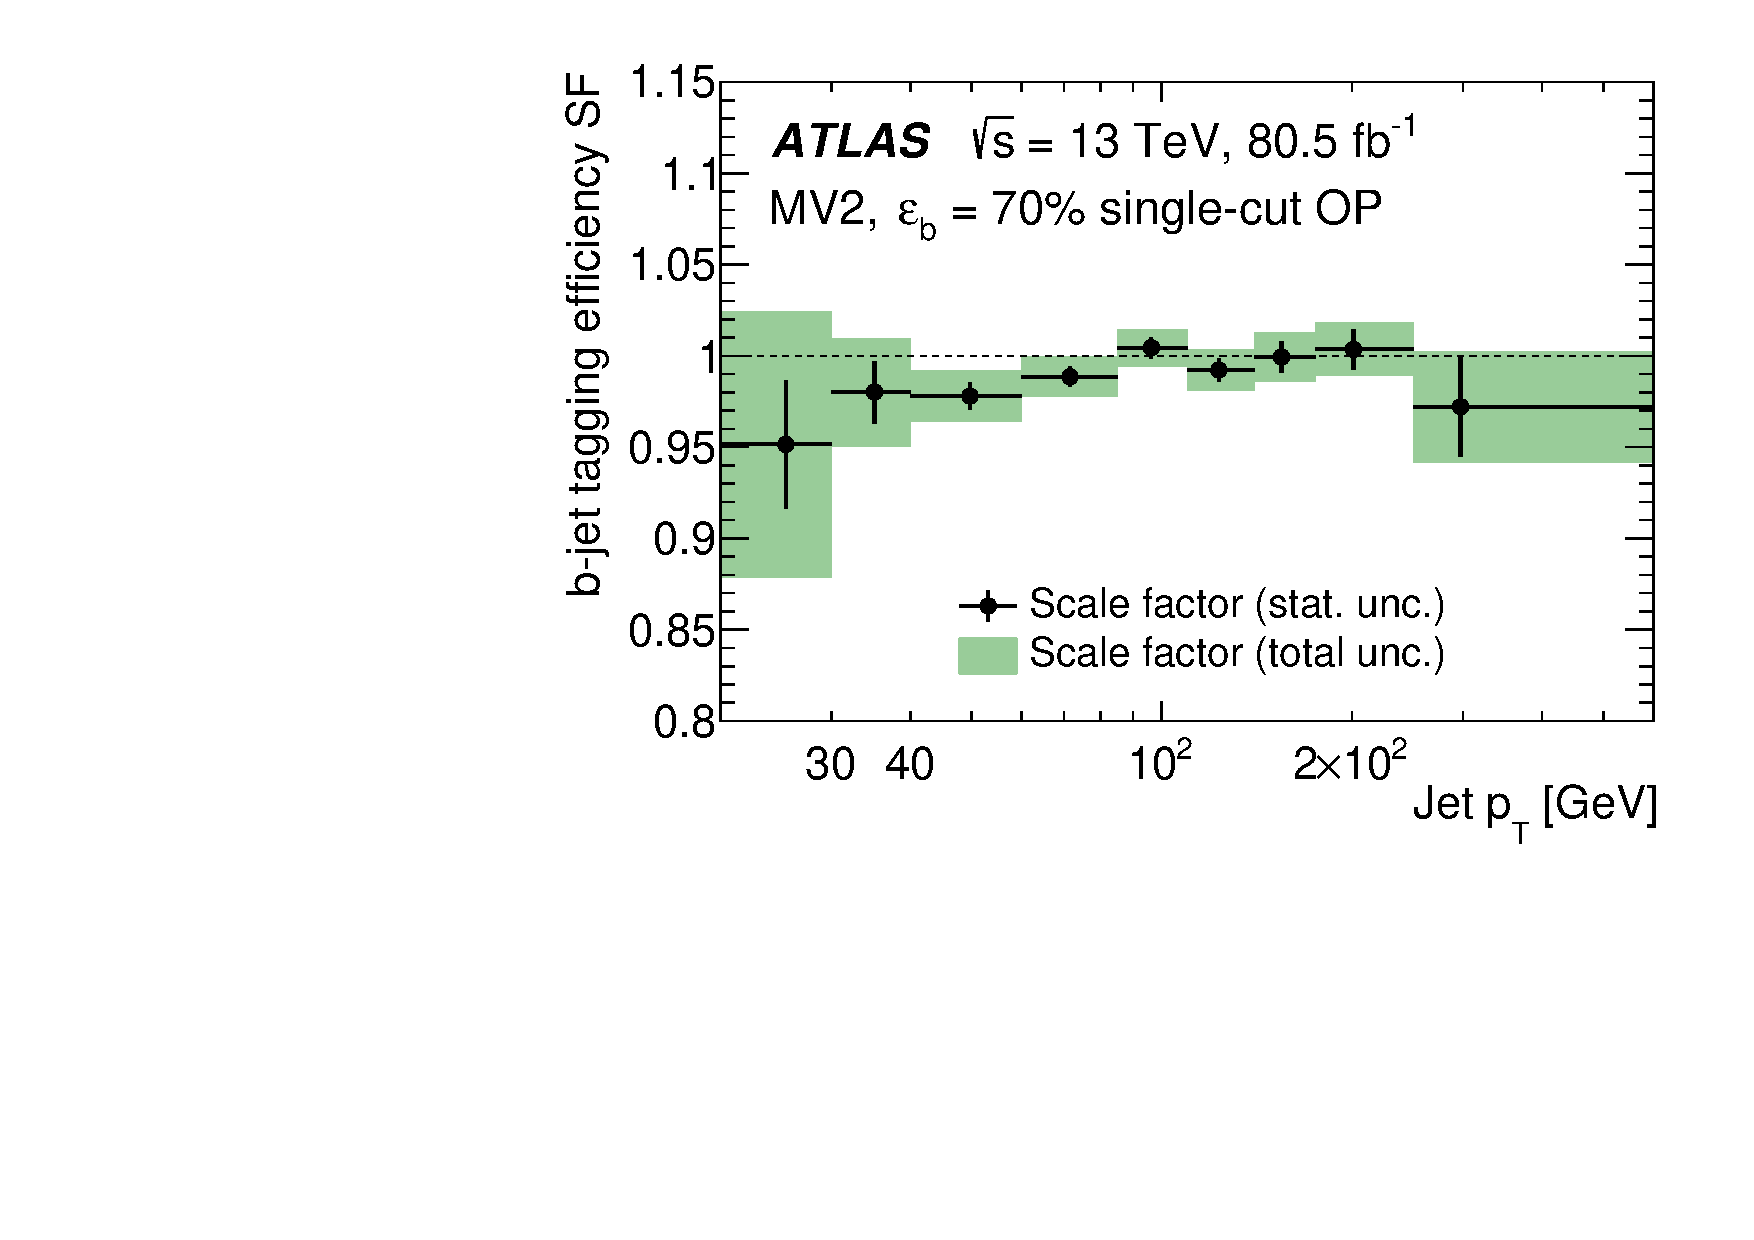
\includegraphics[width=1.\textwidth]{figures/methods/btagging_sf70.pdf}
      \caption{\btagging efficiency simulation-to-data scale factors}
      \label{fig:methods:event-reconstruction:jets:btagging:corrections:sf}
    \end{subfigure}
    \caption{The \btagging efficiency (left) and \btagging efficiency simulation-to-data scale factors (right) for the \SI{70}{\percent} single-cut OP of the MV2 tagger as a function of jet \pt. The efficiency measurement is shown in data (dots) and in simulated \ttbar events (red line), together with the total uncertainty (green band). Figures reproduced from Ref.~\cite{FTAG-2018-01}.}
    \label{fig:methods:event-reconstruction:jets:btagging:corrections}
\end{figure}

\subsubsection{Large-radius calorimeter jets}
\label{sec:methods:event-reconstruction:jets:larger}
The reconstruction of hadronically decaying heavy bosons using a pair of small-radius jets becomes infeasible for boosted objects. The strong collimation of their decay products as a consequence of the Lorentz boost makes it impossible to resolve the decay's partonic sub-structure. As a rule-of-thumb, the separation between the two decay products of a boosted heavy boson with mass \(m\) and transverse momentum \pt can be estimated~\cite{Butterworth2008} as
\begin{align}
    R = \frac{1}{z (1-z)} \times \frac{m}{\pt},
\end{align}
where \(z\), \(1-z\) are the momentum fractions of the two decay products.
As heavy bosons have a larger transverse momentum, their decay products become increasingly collimated, as illustrated in \Cref{fig:methods:event-reconstruction:jets:larger:boosted}.
Therefore, the reconstruction of the boosted object is based on a single jet with large radius parameter, which can fully contain the boosted heavy boson decay.

\begin{figure}[htbp]
    \centering
    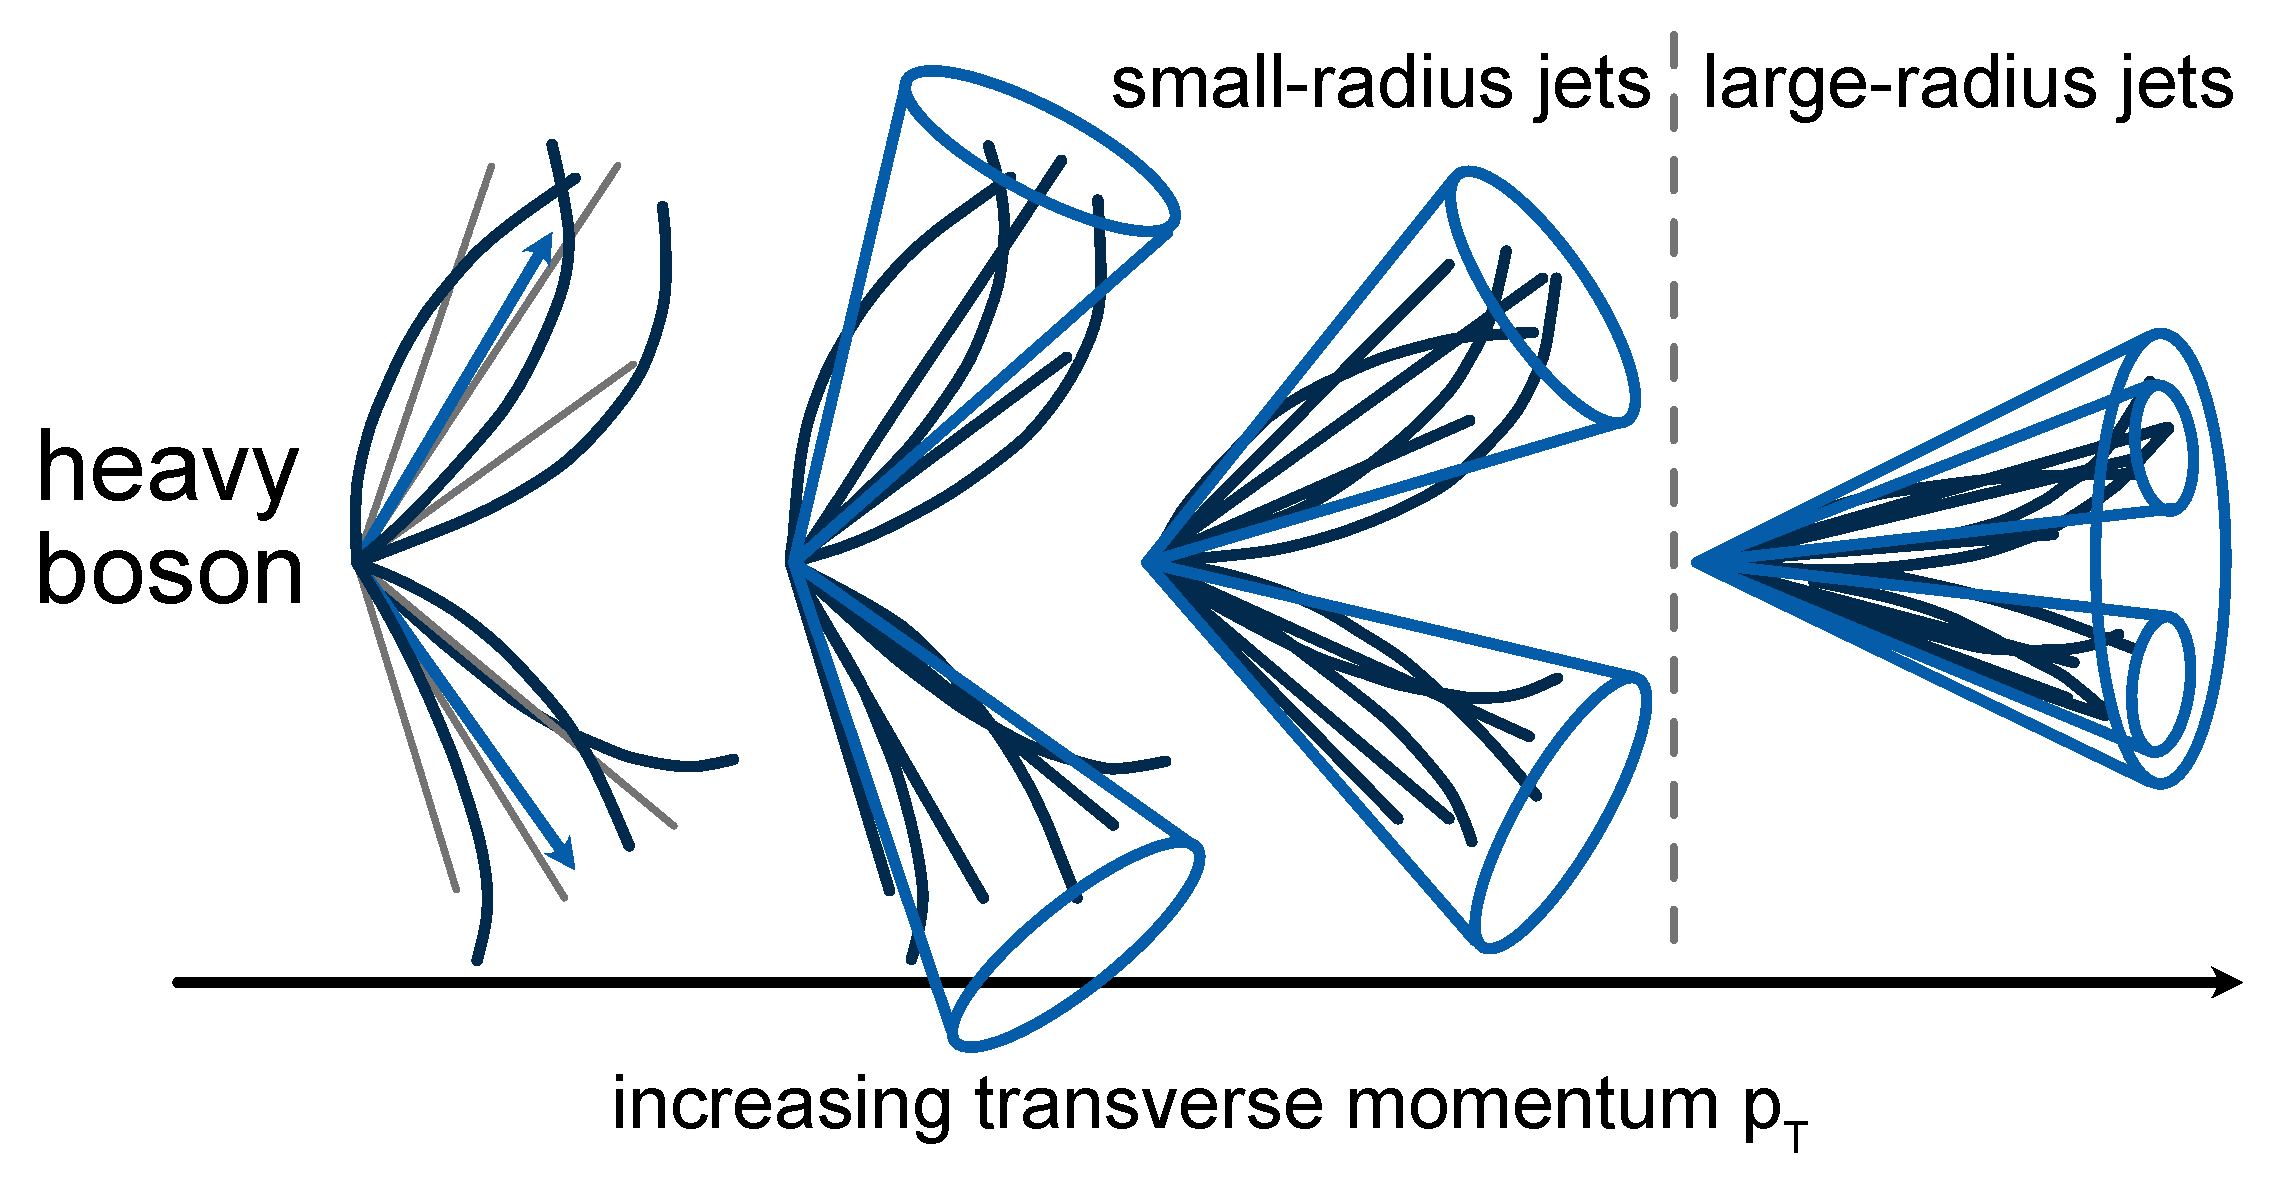
\includegraphics[width=.95\textwidth]{figures/methods/jet_boosted.pdf}
    \caption{Illustration of boosted event topologies: the distance between the decay products of a boosted boson decreases with increasing transverse momentum of the boosted boson.}
    \label{fig:methods:event-reconstruction:jets:larger:boosted}
\end{figure}

The reconstruction and calibration procedure of large-radius jets consists of several stages, which are illustrated by \Cref{fig:methods:event-reconstruction:jets:larger:calibration}.

\begin{figure}[htbp]
	\centering
	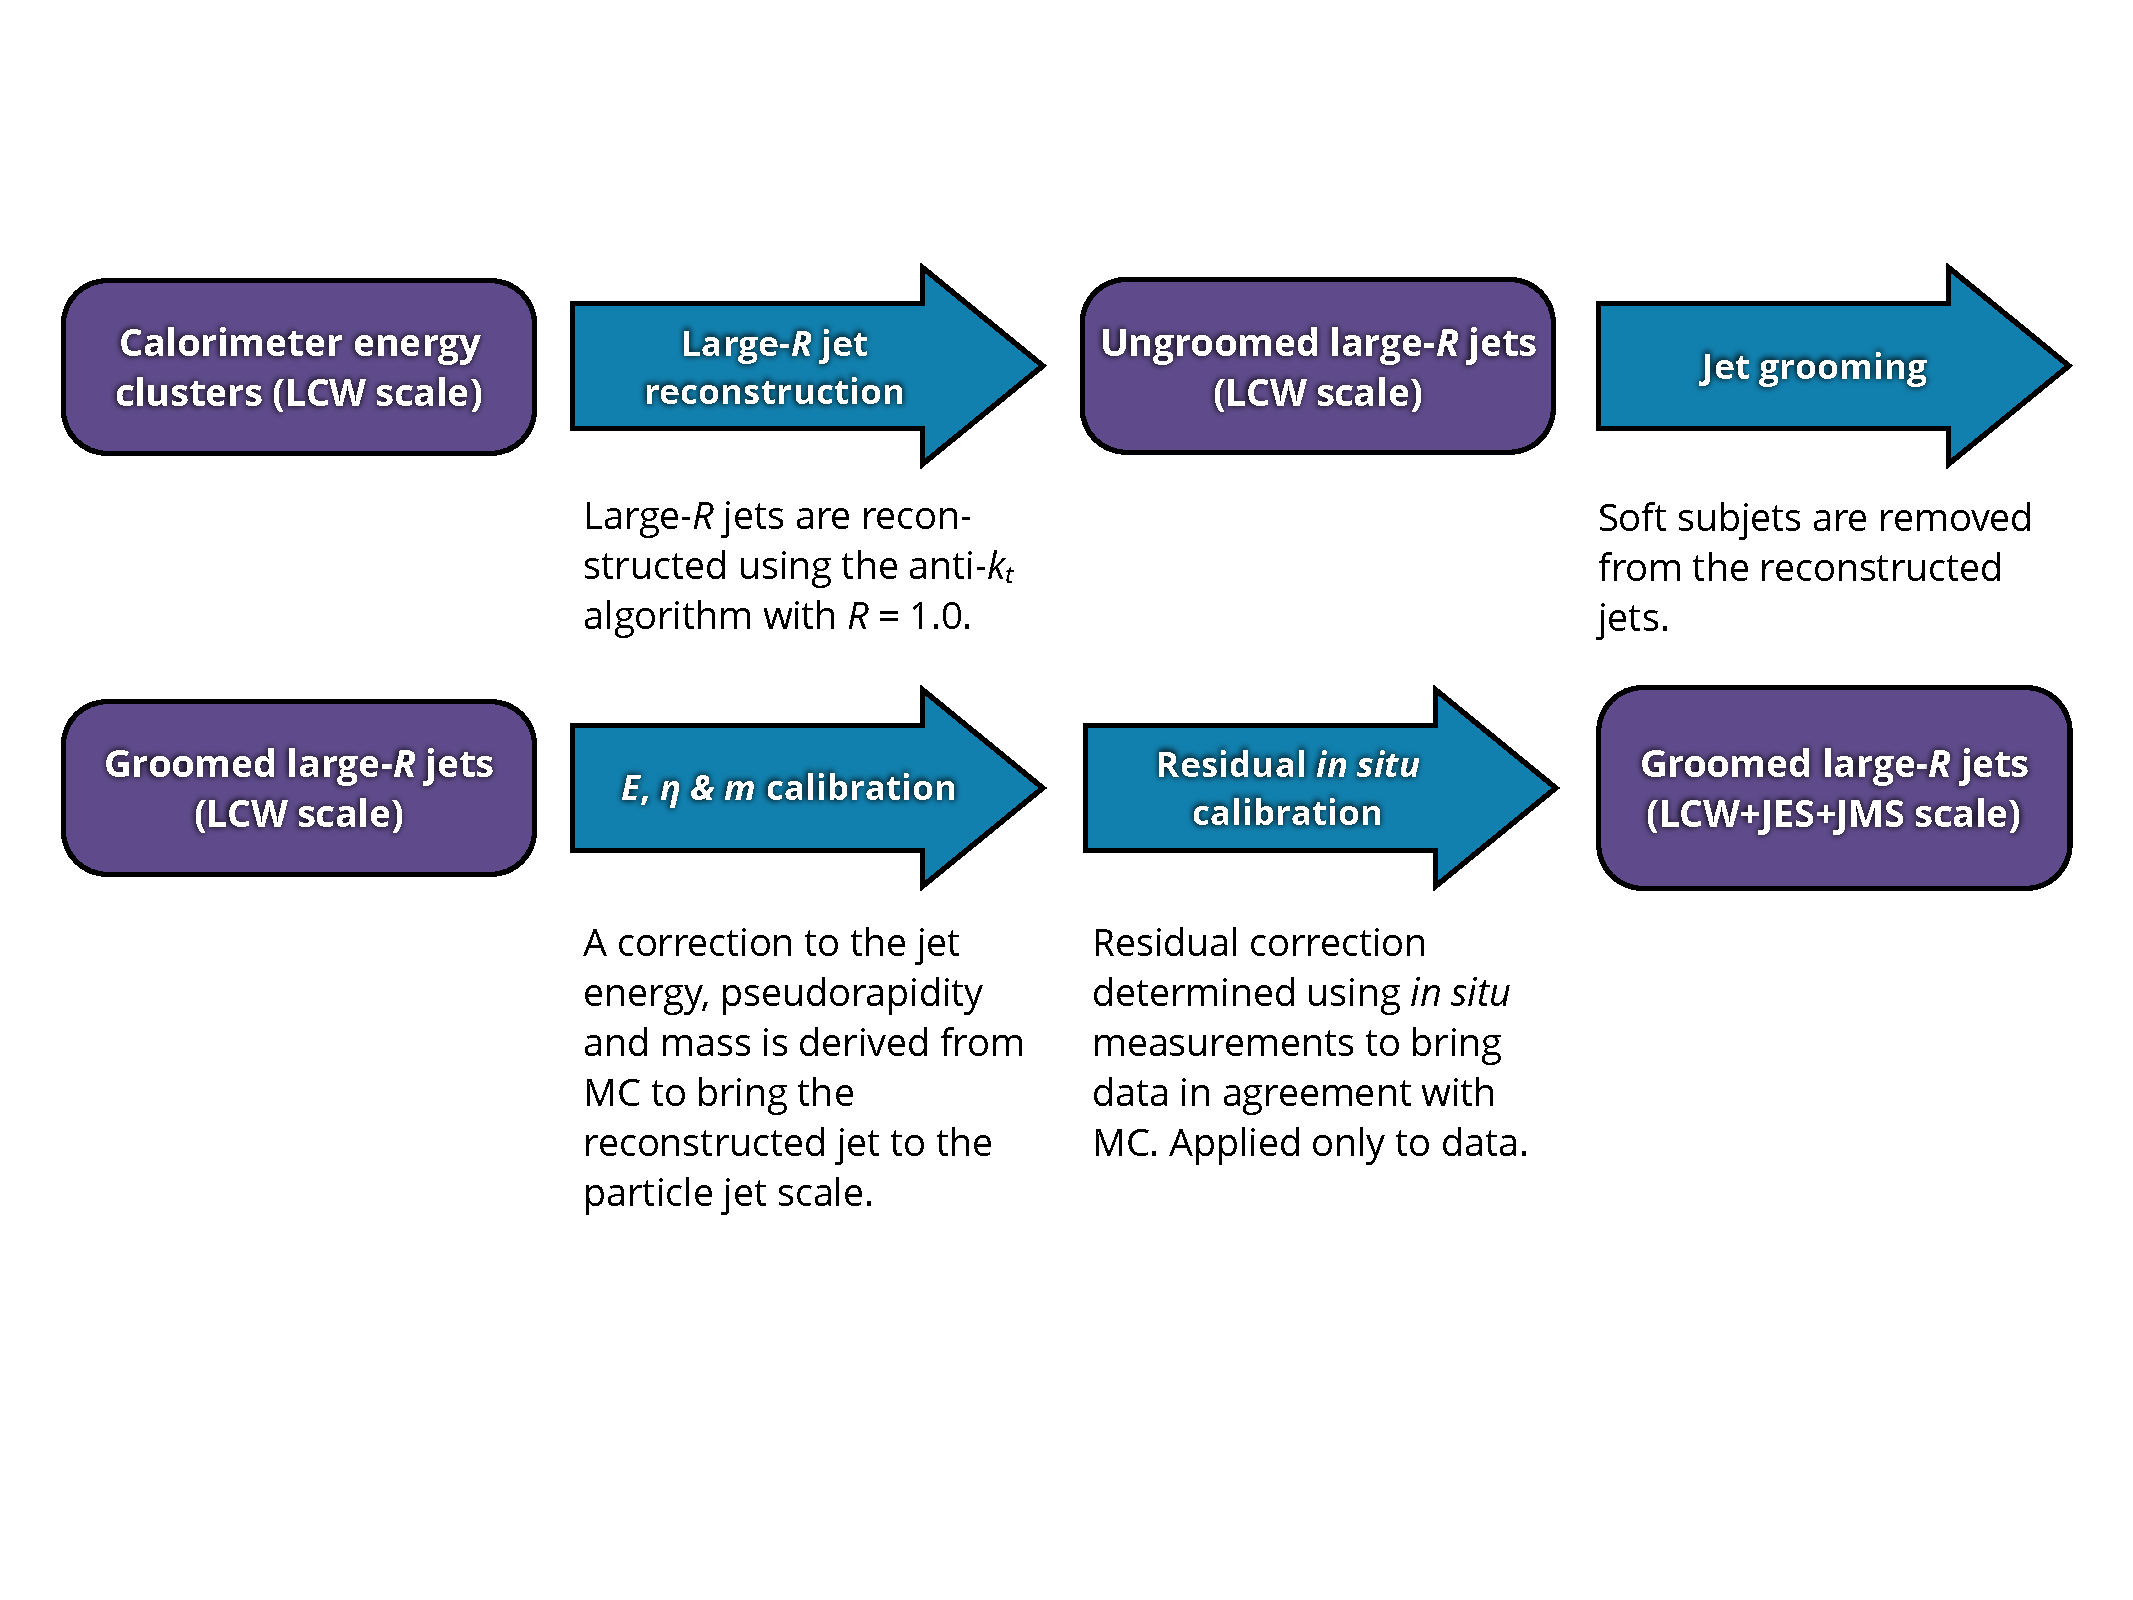
\includegraphics[width=0.95\textwidth]{figures/methods/jet_larger_calibration.pdf}
	\caption{Overview of the large-radius jet reconstruction and calibration procedure. Illustration reproduced from Ref.~\cite{JETM-2018-02}.}
	\label{fig:methods:event-reconstruction:jets:larger:calibration}
\end{figure}

Large-radius jets are reconstructed from topological clusters in the calorimeters, which are calibrated to the hadronic scale in the LCW scheme, using the \antikt algorithm with a radius parameter \(R = 1.0\).

The large radius parameter makes the reconstructed jets particularly susceptible to contamination from pile-up, initial-state radiation, and multiple parton interactions. The contributions of these processes are generally softer  than those of the hard scattering process and can therefore be suppressed by jet grooming algorithms~\cite{Kogler2019}.
Among the large variety of algorithms which has been studied~\cite{Dasgupta2013,Ellis2010,Larkoski2014,Dreyer2018}, the commonly adapted jet trimming algorithm~\cite{Krohn2010} is used to remove soft contaminations of the large-radius jets. All particles in a large-radius jet with radius \(R\) are re-clustered into sub-jets with radius parameter \(R_{\text{sub}} < R\) using the \(k_{\text{T}}\)-algorithm. The resulting sub-jets that satisfy the condition \(\pt^{\text{sub-jet}} > f_{\text{cut}} \pt^{\text{large-radius jet}}\) are kept and merged to form the trimmed large-radius jet. The algorithm is illustrated in \Cref{fig:methods:event-reconstruction:jets:larger:trimming}.

\begin{figure}[htbp]
	\centering
	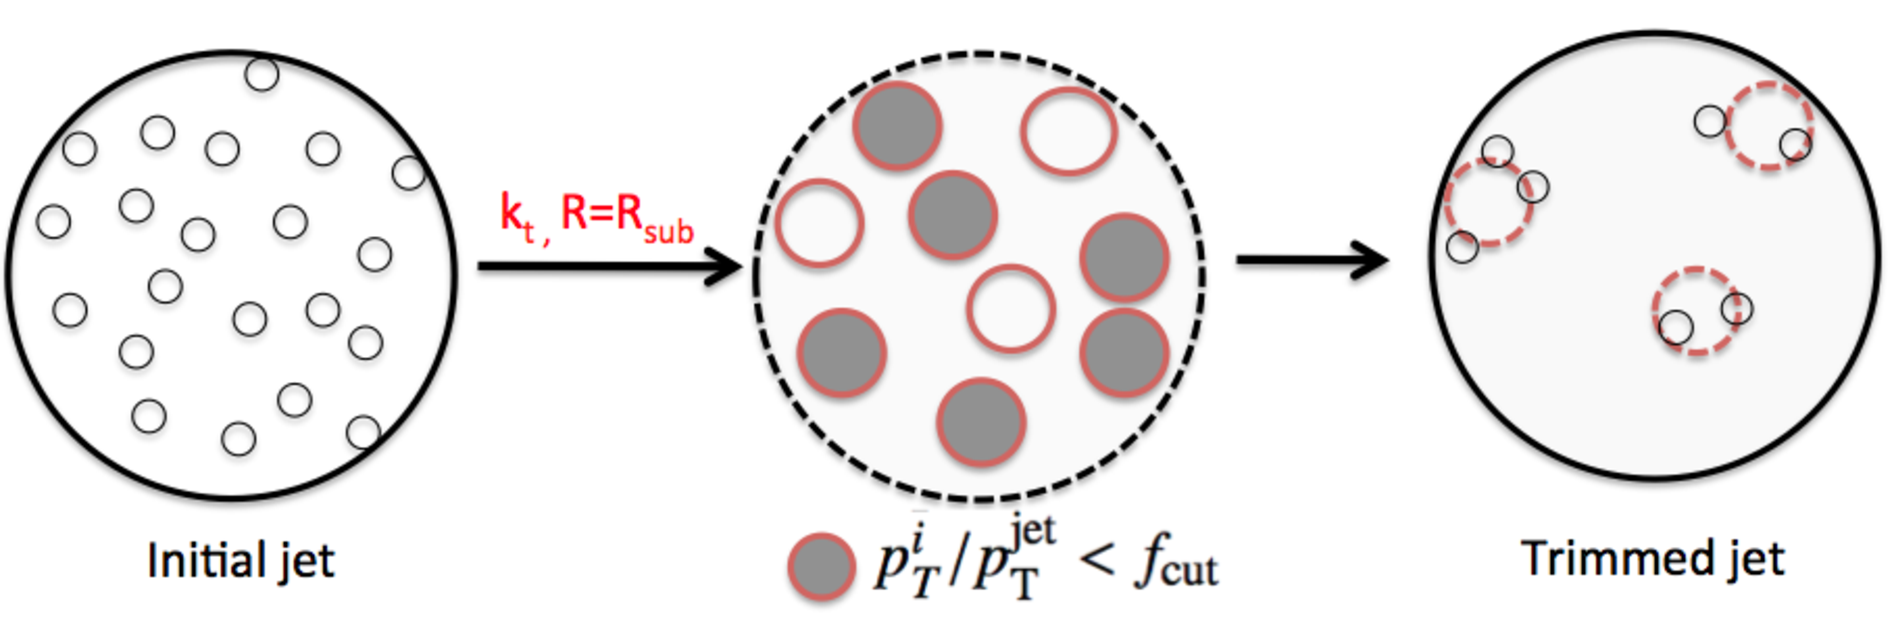
\includegraphics[width=0.95\textwidth]{figures/methods/jet_trimming.pdf}
	\caption{Illustration of the jet-trimming algorithm for large-radius jets. Figure reproduced from Ref.~\cite{PERF-2012-02}.}
	\label{fig:methods:event-reconstruction:jets:larger:trimming}
\end{figure}

The trimmed large-radius jets are calibrated to the energy scale of final-state particles using corrections derived in MC simulations. These simulations correct the \pt, \(\eta\), and the jet mass.
Finally, the jets undergo a residual in-situ calibration using jet response measurements in \HepProcess{\Pp\Pp} collision data. Similar to the small-radius jets, the correction is derived from a statistical combination of data-to-simulation ratios of these response measurements and is applied only to data.

The large-radius jet mass resolution is improved by using both calorimeter and tracking information in the reconstruction.
The calorimeter-based (CA) jet mass is computed from the energies \(E_{i}^{\text{topo}}\) and momenta \(\vec{p}_{i}^{\text{topo}}\) of topological clusters in the calorimeter as
\begin{align}
    m^{\text{CA}} = \sqrt{\left(\sum_{i} E_{i}^{\text{topo}}\right)^2 - \left(\sum_{i} \vec{p}_{i}^{\text{topo}}\right)^2}.
\end{align}

The track-assisted (TA) mass is computed in a similar way from a mass measurement based on ID tracks \(m^{\text{track}}\) but additionally weighted with the ratio of the transverse momenta measured by the calorimeters (\(\pt^{\text{calo}}\)) and the ID (\(\pt^{\text{track}}\)) to account for neutral hadrons. It is defined as
\begin{align}
    m^{\text{TA}} = m^{\text{track}} \times \frac{\pt^{\text{calo}}}{\pt^{\text{track}}}.
\end{align}

The combined jet mass is defined as the weighted least-squares combination of the CA and TA mass definitions
\begin{align}
    m^{\text{comb}} = \frac{\sigma_{\text{CA}}^{-2}}{\sigma_{\text{CA}}^{-2} + \sigma_{\text{TA}}^{-2}} \times m^{\text{CA}} + \frac{\sigma_{\text{TA}}^{-2}}{\sigma_{\text{CA}}^{-2} + \sigma_{\text{TA}}^{-2}} \times m^{\text{TA}},
\end{align}
with the respective mass resolutions \(\sigma_{\text{CA}}\) and \(\sigma_{\text{TA}}\).

The combined jet mass definition improves the jet mass resolution and reduces the systematic uncertainties, as shown in \Cref{fig:methods:event-reconstruction:jets:larger:combinedmass}.

\begin{figure}[htbp]
  \centering
  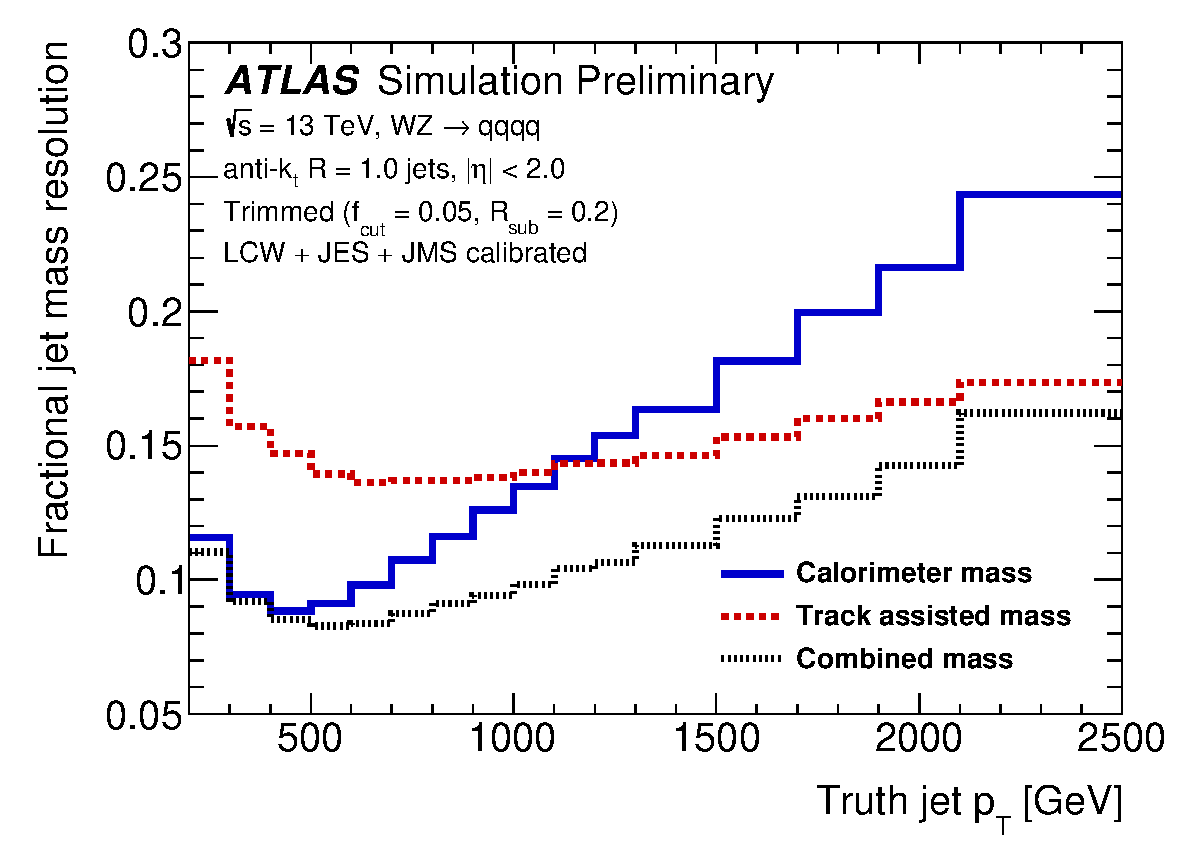
\includegraphics[width=0.75\textwidth]{figures/methods/combinedmass.pdf}
  \caption{The fractional jet mass resolution, defined as half the ratio of the \SI{68}{\percent} confidence interval inter-quantile range of the jet mass response distribution and the median jet response, estimated in dependence of the truth jet \pt using simulated hadronic decays of diboson processes. Figure reproduced from Ref.~\cite{JETM-2017-002}.}
  \label{fig:methods:event-reconstruction:jets:larger:combinedmass}
\end{figure}


\subsubsection{Track jets}
\label{sec:methods:event-reconstruction:jets:trackjets}
The track jets supplement the reconstruction of boosted heavy bosons based on large-radius jets by enabling the identification of the large-radius jet's flavour content.

Track jets with fixed radius parameter are reconstructed using the \antikt algorithm with \(R=0.2\) on ID tracks originating from the PV with \(\pt >  \SI{0.5}{\giga\electronvolt}\) and \(\abs{\eta} < 2.5\). The tracks are required to have at least seven hits in total in the SCT and PXD detectors, no more than one hit shared by multiple tracks in the PXD detector, and at most one missing hit in the PXD or two missing hits in the SCT detectors.
An additional requirement on the longitudinal impact parameter \(\abs{z_0 \sin \theta} < \SI{3}{\milli\meter}\) with respect to the PV reduces the pile-up contribution.

The smaller radius parameter and superior angular resolution of the tracking detector allow resolving the partonic substructure of the heavy boson decay even in dense environments.
However, for substantially boosted event topologies, even the track jets can overlap if they are reconstructed with a fixed radius parameter. The problem of track jet merging is overcome by the use of a modified jet algorithm in which the radius parameter decreases with increasing jet transverse momentum as the jet is being formed. The scaling of the effective jet radius
\begin{align}
R_{\text{eff}} = \frac{\rho}{\pt},
\end{align}
with the transverse momentum of the pseudo-jet \pt as it is being formed (c.f. \Cref{sec:pp:jets}) is determined by the parameter \(\rho = \SI{30}{\giga\electronvolt}\). The effective jet radius is bounded by \(0.02 \leq R_{\text{eff}} \leq  0.4\). The resulting jets are referred to as variable-radius (VR) track jets~\cite{Krohn2009,ATL-PHYS-PUB-2017-010}. The reconstruction of VR track jets in comparison to that of FR track jets with radius parameter \(R=0.2\) is illustrated in \Cref{fig:methods:event-reconstruction:jets:trackjets:illustration}.

\begin{figure}[hbtp]
  \centering
  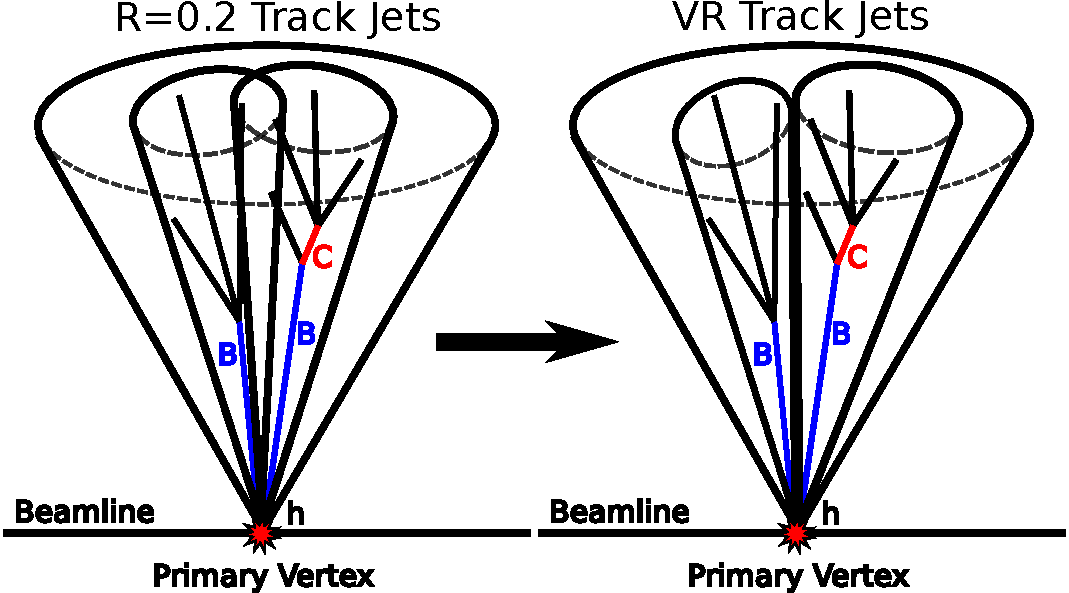
\includegraphics[width=0.65\textwidth]{figures/methods/vrtrackjets_cartoon.pdf}
  \caption{Illustration of the sub-jet reconstruction using either fixed radius (left) or variable radius (right) track jets. Figure reproduced from Ref.~\cite{ATL-PHYS-PUB-2017-010}.}
  \label{fig:methods:event-reconstruction:jets:trackjets:illustration}
\end{figure}

The track jets are uniquely associated with a large-radius jet using the ghost-association technique, in which ghost particles --- copies of the track jet four-momentum with vanishing momentum --- are added to the inputs of the large-radius jet algorithm. This procedure allows for the unique association of the track jets with a large-radius jet by identifying the ghost particles associated with the non-trimmed large-radius jet.

Track jets undergo no calibration procedure, as the kinematic properties of the heavy boson are reconstructed from large-radius jet information and the track jets are only used for the identification of the large-radius jet flavour.
Similar to small-radius jets, the MV2 \btagging algorithm is used to identify track jets originating from \bquarks.
The \btagging efficiency and the misidentification rates for \cjets and light-flavour jets are compared between data and MC to derive corrections for simulated events.


\subsection{Tau leptons}
\label{sec:methods:event-reconstruction:taus}
As \Pgt leptons have a proper decay length of \(c\tau = \SI{87}{\micro\meter}\)~\cite{Tanabashi2018} and subsequently decay within the LHC beam pipe, their leptonic decays are reconstructed as stable electrons or muons.

The hadronically decaying \Pgt leptons are reconstructed as small-radius jets and identified using MVA techniques, conceptually similar to \btagging.
\Pgt decays exhibit a characteristic signature of either 1 or 3 charged hadrons collimated along the jet axis accompanied by neutral hadrons. A combination of boosted decision trees targets the 1-prong and 3-prong \Pgt decay modes and allows for the definition of working points with increasing purity and decreasing efficiency, including the \textsc{Loose} BDT OP which is used in the dark matter searches presented in this dissertation.

\subsection{Missing transverse momentum}
\label{sec:methods:event-reconstruction:met}
The missing transverse momentum \met is a key observable when searching for undetected objects such as dark matter particles or neutrinos. The almost hermetic design of the ATLAS detector enables the reconstruction of these objects via the transverse momentum balance in a collision event. The composite nature of the protons undergoing the collision restricts the knowledge of the momentum before the collision to the transverse plane, where it is zero since the full momentum is aligned in the beam direction. Thus, any momentum imbalance in the transverse plane after the collision can be attributed to undetected objects.

The missing transverse momentum is defined as the negative sum of all physics object transverse momentum vectors and a component due to the track soft term (TST)
\begin{align}
\met = - \left| \sum_{e, \mu, \gamma, \tau, \text{jets}} \vec{p}_{\text{T}} \, + \sum_{\text{soft term}} \vec{p}_{\text{T}} \right|.
\end{align}
A high reconstruction efficiency for objects entering the \met computation is desirable, therefore loose object definitions are employed when calculating the missing transverse momentum.
The TST  is composed of all tracks not associated with physics objects and is particularly relevant for estimating the \met scale and resolution.

As \met is of paramount importance not only for dark matter searches, several OPs are defined for the competing needs of various analyses in terms of pile-up suppression and \met resolution.
\begin{itemize}
	\item \textsc{Loose}. The \met calculation includes jets with \(\pt > \SI{20}{\giga\electronvolt}\) and \(\abs{\eta} < 4.5\). Jets with \(\pt < \SI{60}{\giga\electronvolt}\) and \(\abs{\eta} < 2.4\) are required to pass the Jet Vertex Tagger (JVT) selection with a JVT score of \(\text{JVT} >  0.59\).
	\item \textsc{Tight}. The \met calculation includes the jets described in the \textsc{Loose} OP definition. In addition, forward jets (\(2.4 < \abs{\eta} < 4.5\) must satisfy \(\pt > \SI{30}{\giga\electronvolt}\).
\end{itemize}
The \textsc{Tight} OP offers better pile-up suppression at the cost of inferior \met resolution for low pile-up events with respect to the \textsc{Loose} OP.
\Cref{fig:methods:event-reconstruction:met:resolution} shows the \met resolution in dependence of the number of primary vertices \(N_{\textsc{PV}}\) in the event for the two OPs.

\begin{figure}[hbtp]
  \centering
  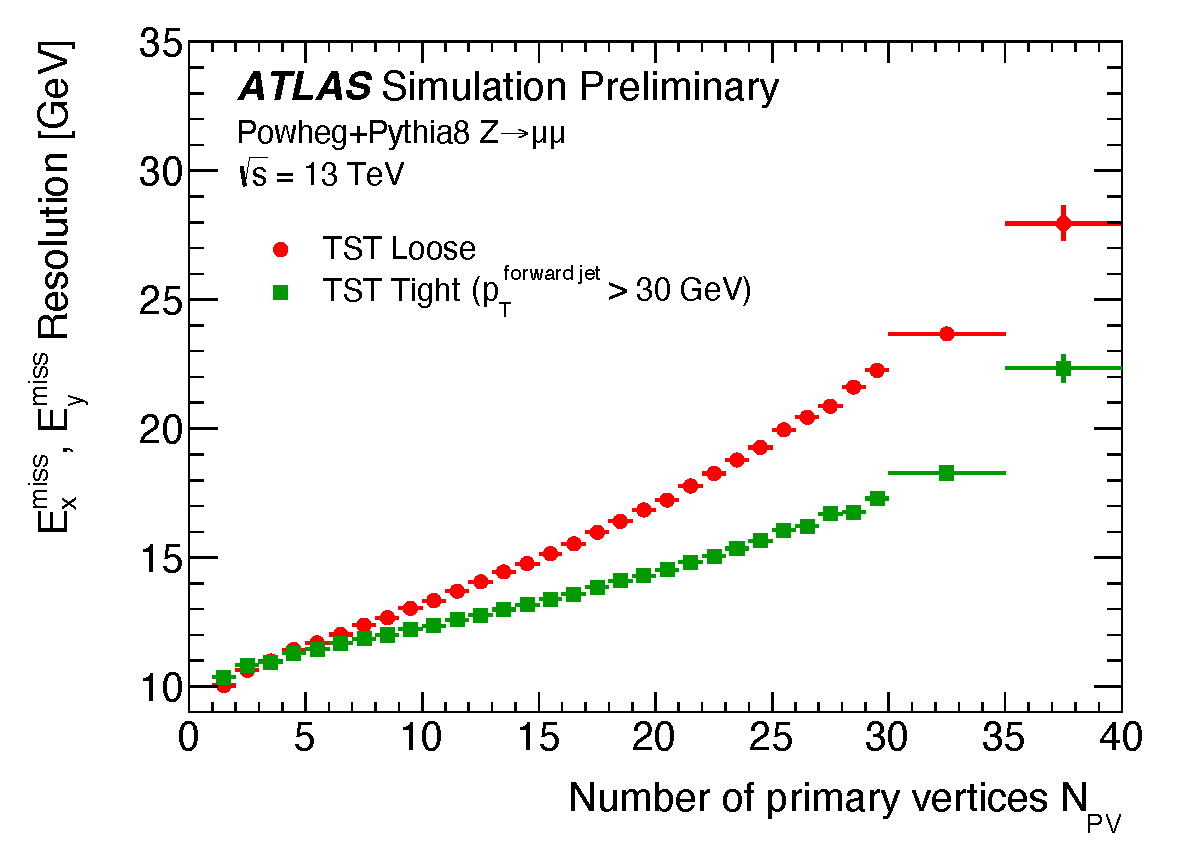
\includegraphics[width=0.7\textwidth]{figures/methods/met_resolution.pdf}
  \caption{Distribution of the \met resolution in dependence of the number of primary vertices \(N_{\textsc{PV}}\) in the event for \met reconstructed with the \textsc{Loose} and \textsc{Tight} operating points in \HepProcess{\PZ \to \Pgm\Pgm} events. Figure adapted from Ref.~\cite{ATLAS-CONF-2018-023}.}
  \label{fig:methods:event-reconstruction:met:resolution}
\end{figure}

A related variable \mpt is defined as the negative vectorial sum of the transverse momenta of all tracks associated with the primary vertex. This variable is used to reduce beam-induced and non-collision backgrounds.

The \textbf{missing transverse momentum significance} is used to separate events in which the reconstructed missing transverse momentum \met is genuinely coming from dark matter particles or neutrinos from events with fake \met being observed due to contributions from particle-measurement or resolution effects.
In addition to historical definitions of the \met significance, where the scalar sum of objects entering the \met calculation \(\sum \met\) serves as an event-based approximation to the full \met resolution, an object-based \met significance definition is considered.

The object-based \met significance \(\mathcal{S}\)~\cite{ATLAS-CONF-2018-038} takes into account the resolutions and full correlation among all objects entering the \met reconstruction.
In a coordinate system, which is rotated parallel (longitudinal L) and perpendicular (transverse T) to the direction of the missing transverse momentum vector, the object-based \met significance definition can be written as
\begin{align}
    \mathcal{S}^2 & = %
	    \begin{pmatrix} \met & 0 \end{pmatrix} %
	    \begin{pmatrix} \sigma_{L}^{2} & \rho_{LT} \sigma_{L} \sigma_{T} \\ \rho_{LT} \sigma_{L} \sigma_{T} & \sigma_{T}^{2} \end{pmatrix}^{-1} %
	    \begin{pmatrix} \met \\ 0 \end{pmatrix} \\ %
               & = \frac{\left(\met\right)^2}{\sigma_{L}^{2}\left(1-\rho_{LT}^{2}\right)},
\end{align}
where \(\sigma_{L}^{2}\) and \(\sigma_{T}^{2}\) are the total variances in the longitudinal (L) and transverse (T) directions to the \(\vec{\met}\) vector, respectively, and \(\rho_{LT}\) is the correlation factor of the two measurements. These variances consider all fluctuations in the direction (L) or perpendicular (T) to the direction of the reconstructed \met from the hard objects entering the \met calculation.

A high value of \(\mathcal{S}\) is an indication that the observed \met in the event cannot be accounted for by resolution smearing alone, suggesting that the event may contain unseen objects such as neutrinos or dark matter particles.

\Cref{fig:methods:event-reconstruction:metsignificance:performance} illustrates the performance of the object-based \met significance in comparison to an event-based definition of \met significance and \met itself. The object-based \met significance definition is clearly superior, as it provides rejection of over \SI{98}{\percent} of the background processes with fake \met while retaining a signal efficiency over \SI{80}{\percent}. In comparison, \met and the event-based \met significance provide background rejection of \SI{55}{\percent} and \SI{75}{\percent}, respectively~\cite{ATLAS-CONF-2018-038}.

\begin{figure}[htbp]
	\centering
	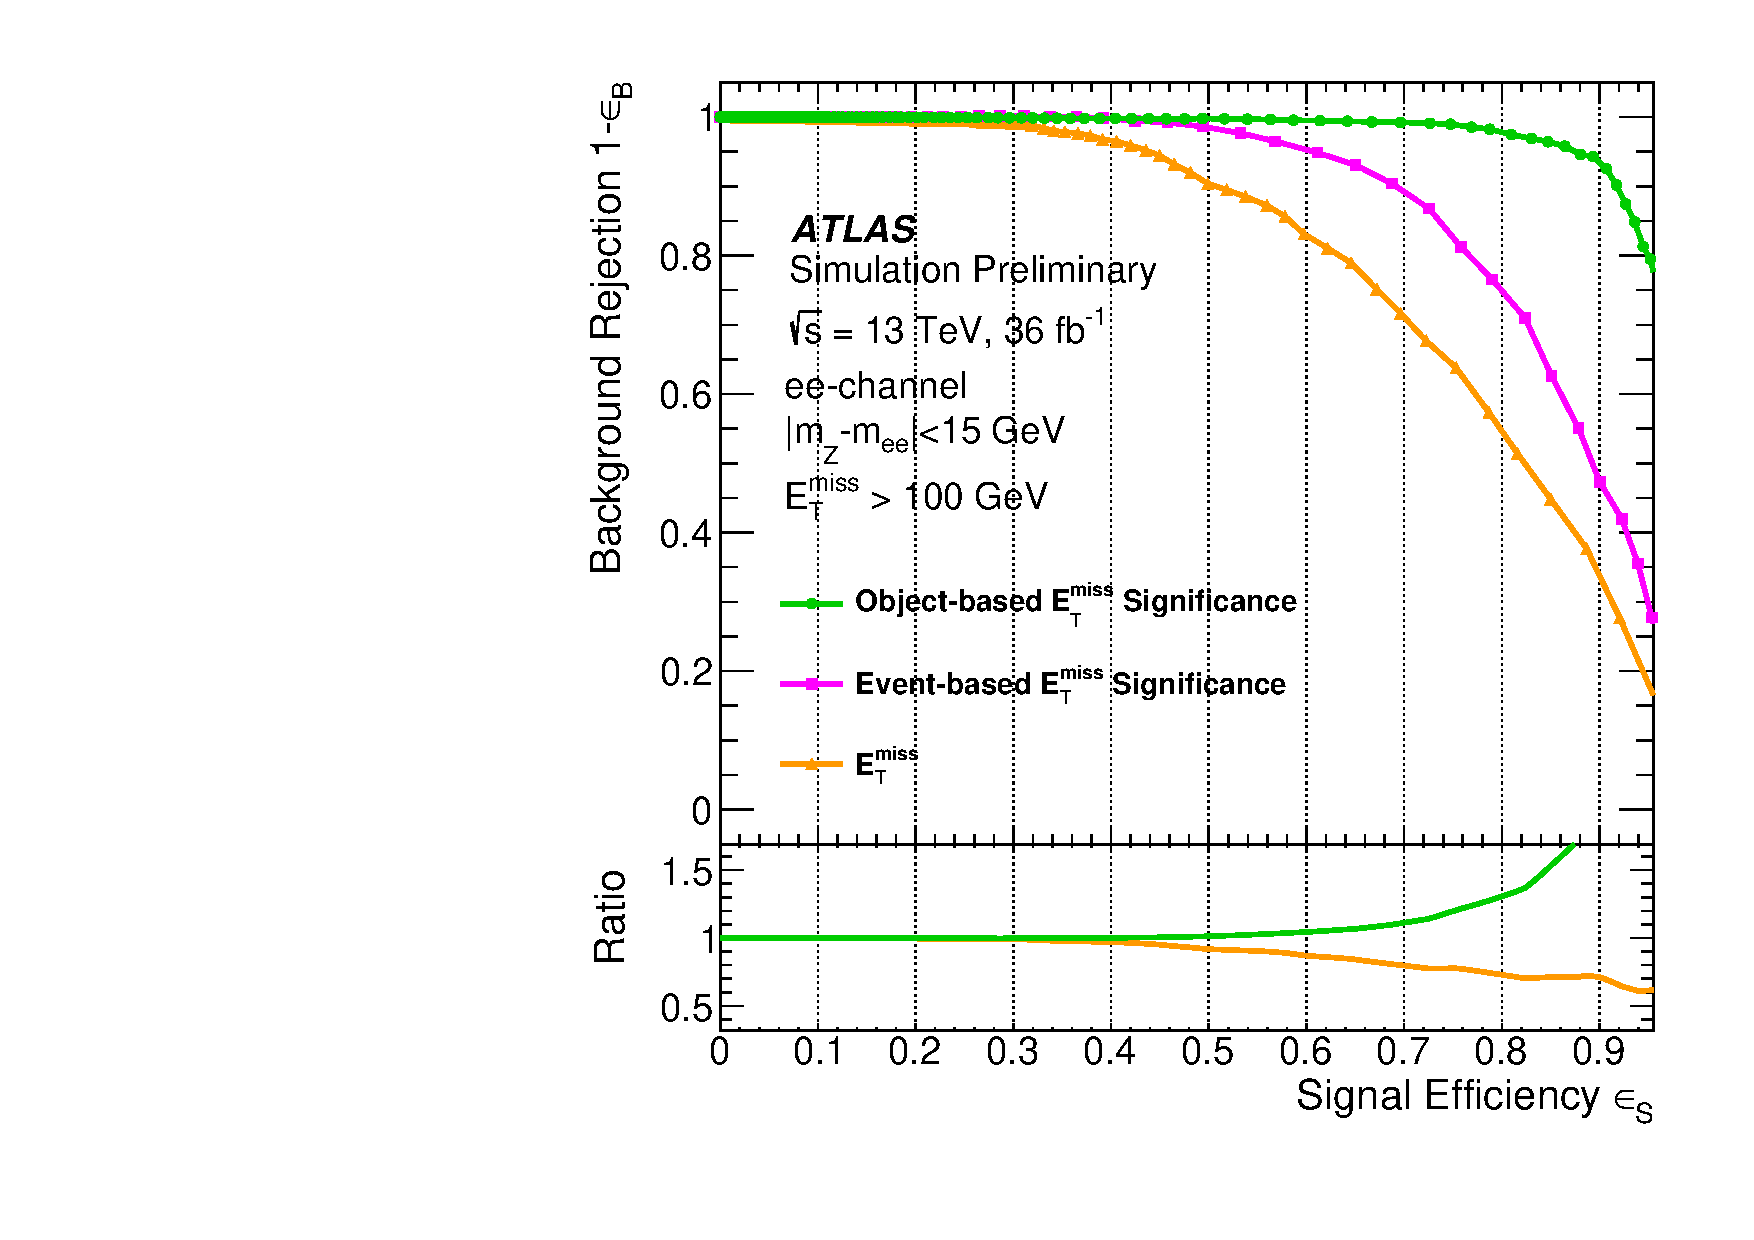
\includegraphics[width=0.75\textwidth]{figures/methods/met_significance.pdf}
	\caption{Performance of the \met significance in terms of background rejection versus signal efficiency in simulated \HepProcess{\PZ \to \Pe \Pe} and \HepProcess{\PZ \to \Pe \Pe \Pgn \Pgn} samples with a \HepProcess{\PZ to \Pe \Pe} selection. The performance is shown for \met~(orange), event-based \met significance~(pink), and object-based \met significance~(green) as discriminants in events with a \(\met > \SI{100}{\giga\electronvolt}\) pre-selection. The lower panel shows the ratio of other definitions to the event-based \met significance. Figure reproduced from Ref.~\cite{ATLAS-CONF-2018-038}.}
	\label{fig:methods:event-reconstruction:metsignificance:performance}
\end{figure}

\newpage

\section{Statistical methods}
\label{sec:methods:statistics}
Common statistical methods used in all searches for dark matter presented in this dissertation are introduced in this section.

The simplest definition of a fit is based on a statistical model only considering the total number of selected events. Typically, the statistical model is based on simulated samples of the signal (\(S\)) and background (\(B\)) processes, which provide the predicted event yields for the respective processes.
A maximum-likelihood fit of the model to data determines the best-fit values of the parameter of interest (POI) and the nuisance parameters (NP) \(\vec{\theta}\). The POI is typically taken to be the signal strength \(\mu\), which is defined as the ratio of the signal cross section to a reference signal cross section predicted by theory. The NPs denote further parameters in the model which are subject to uncertainties, e.g. the individual background normalisation parameters.
The total predicted event yield is
\begin{align}
    N^{\text{exp}} (\mu, \vec{\theta}) = \mu S(\vec{\theta}) + B(\vec{\theta}).
\end{align}
The sensitivity to signal processes can be enhanced by considering not only the total event yield but distributions of discriminating variables. These variables are chosen to provide strong separation between signal and background processes. The statistical model for such a fit based on binned distributions of the discriminating variables is described by the likelihood function
\begin{align}
	\mathcal{L}(N^{\text{obs}} | \mu, \vec{\theta}) = %
	\text{Pois}(N^{\text{obs}} | N^{\text{exp}} (\mu, \vec{\theta})) %
	\times \left[ %
		\prod_{i \in \text{bins}} \frac{\mu S_i(\vec{\theta}) + B_i(\vec{\theta})}{N^{\text{exp}} (\mu, \vec{\theta})}
	\right] %
	\times \prod_{\theta_{i} \in \vec{\theta}} f(0 | \theta_{i}),
	\label{eq:methods:statistics:likelihood}
\end{align}
where \(N^{\text{obs}}\) denotes the total observed event yield and \(S_{i}\), \(B_{i}\) denote the number of predicted signal and background events in bin \(i\), respectively.
The systematic uncertainties are implemented as the NPs \(\theta_{i}\) with the associated probability density functions \(f(0|\theta_{i})\).
These are parametrised as standard Gaussian prior distributions with the expectation value \(\theta_{i}\), or in the case of normalisation uncertainties as Log-normal distributions to ensure a positive value of the likelihood function.

A common technique to reduce the uncertainties on the background modelling is the use of control region data.
Auxiliary measurements in dedicated selections which are enriched in the respective background processes provide constraints on the normalisation of the simulated backgrounds.

The searches presented in this dissertation use a profile likelihood fit which is based on \Cref{eq:methods:statistics:likelihood} and is implemented using the \textsc{HistFactory}~\cite{Cranmer2012} software.
The results are obtained by maximising the likelihood function \(\mathcal{L}(N^{\text{obs}} | \mu, \theta)\) under consideration of the likelihood ratio test statistic \(q_{\mu}\). The latter is the most powerful test statistic one can construct~\cite{Neyman1933} and is defined by
\begin{align}
    q_{\mu} = - 2 \ln{\left(\frac{\mathcal{L}(\mu, \doublehat{\vec{\theta}})}{\mathcal{L}(\hat{\mu}, \hat{\vec{\theta}})}\right)},
\end{align}
where \(\mathcal{L}(\mu, \doublehat{\vec{\theta}})\) is maximised over all NPs for a given value of \(\mu\) and \(\mathcal{L}(\hat{\mu}, \hat{\vec{\theta}})\) denotes the global maximum of the full parameter space \(\mu, \vec{\theta}\). Here, \(\doublehat{\vec{\theta}}\) is referred to as the conditional maximum-likelihood estimator of \(\vec{\theta}\), whereas \(\hat{\mu}\) and \(\hat{\vec{\theta}}\) are referred to as the unconditional maximum-likelihood estimators of \(\mu\) and \(\vec{\theta}\), respectively.

The test statistic \(q_{\mu}\) can be used to test a given signal strength \(\mu\) hypothesis.
Searches for new physics processes, which manifest as a significant excess over the SM background, consider the ``background-only'' hypothesis with \(\mu=0\) as the null hypothesis. The test for discovery is performed by rejecting the null hypothesis using the test statistic
\begin{align}
    q_{0} = \begin{cases} - 2 \ln \left(\frac{\mathcal{L}(0, \doublehat{\vec{\theta}})}{\mathcal{L}(\hat{\mu}, \hat{\vec{\theta}})}\right) & \text{for } \hat{\mu} > 0 \\ 0 & \text{for } \hat{\mu} \leq 0. \end{cases}
\end{align}
Large values of \(q_{0}\) correspond to more observed events than could be explained by ``background-only'' hypothesis, suggesting the presence of a signal.

Typically, tests for discovery are stated in terms of the significance
\begin{align}
Z_{\mu} = 1 - \Phi^{-1}(1 - p_{\mu}),
\end{align}
which is defined by the inverse of the cumulative distribution of the standard Gaussian \(\Phi^{-1}\).

If no excess is found in these searches, constraints on the parameter space of specific models for the new physics processes can be set using a different hypothesis test. The test for exclusion is performed by rejecting the ``signal + background'' hypothesis, using the test statistic
\begin{align}
q_{\mu} = \begin{cases} -2 \ln{\left(\frac{\mathcal{L}(\mu, \doublehat{\vec{\theta}})}{\mathcal{L}(0, \hat{\vec{\theta}})}\right)} & \text{for } \hat{\mu} \leq 0 \\ -2 \ln{\left(\frac{\mathcal{L}(\mu, \doublehat{\vec{\theta}})}{\mathcal{L}(\hat{\mu}, \hat{\vec{\theta}})}\right)} & \text{for } 0 < \hat{\mu} \leq \mu \\ 0 & \text{for } \hat{\mu} > \mu.  \end{cases}
\end{align}
Here, the additional condition for \(\hat{\mu}\) avoids considering an excess in data incompatible with the ``signal + background'' hypothesis.
Large values of \(q_{\mu}\) indicate smaller compatibility of the ``signal + background'' hypothesis and the observed data.
The fact that the test-statistic is defined to be non-zero only for \(\hat{\mu} \leq \mu\) implies that only upper limits on \(\mu\) are considered.

The result of the hypothesis test is described by the \(p\)-value
\begin{align}
    p_{\mu} = \int_{q_{\mu}^{\text{obs}}} f(q_{\mu} | \mu) \dd{q_{\mu}},
\end{align}
which quantifies the level of disagreement between the observed data and the statistical model defined by the probability density function \(f(q_{\mu | \mu})\) of \(q_{\mu}\) for a signal strength \(\mu\).

Corresponding \(p\)-values for the ``background-only'' (\(b\)) and the ``signal + background'' (\(s+b\)) hypotheses for a given \(q_{\mu}^{\text{obs}}\) are defined by
\begin{align}
    p_{b} &= \int_{-\infty}^{q_{\mu}^{\text{obs}}} f(q_{\mu} | b) \dd{q_{\mu}} \\
    p_{s+b} &= \int_{q_{\mu}^{\text{obs}}}^{\infty} f(q_{\mu} | s + b) \dd{q_{\mu}}.
\end{align}

These definitions, however, might lead to accidental exclusion of signals for searches which are insensitive to those signals. This might occur if, for instance, there is a downward fluctuation in data relative to the expectation of the background-only hypothesis.
The accidental rejection of signal hypotheses can be avoided by using the \(\text{CL}_{s}\) method~\cite{Read:2002hq}, in which the \(p_{s+b}\) value is weighted by a penalty factor that increases with decreasing sensitivity. The \(\text{CL}_{s}\) value is defined by
\begin{align}
    \text{CL}_{s} = \frac{p_{s+b}}{1 - p_{b}}.
\end{align}
Adopting the \(\text{CL}_{s}\) definition, a point in the parameter space of a model is excluded with confidence level \(1 - \alpha\) if one finds \(\text{CL}_{s} < \alpha\). Evidently, the \(\text{CL}_{s}\) is more conservative, as the \(\text{CL}_{s}\)-based exclusion criterion is more stringent than the usual requirement \(p_{\mu} < \alpha\).
However, it should be pointed out that \(\text{CL}_{s}\) limits have no well-defined coverage and should be interpreted such that the probability of having falsely excluded a signal is less than \(\alpha\).

The observed value of the test statistic \(q_{\mu}^{\text{obs}}\) will differ in independent experiments, as it is subject to statistical fluctuations. When computing the expectation value of \(q_{\mu}\), the underlying probability distribution of the test statistic can in general not be evaluated analytically. It can, however, be approximated.
The approximation can be based on evaluating a large number of simulated toy experiments. Although, in principle, these replicas enable the determination of the expectation value of \(q_{\mu}\) with arbitrarily high precision, it comes at the price of high computational cost.

The Asimov method~\cite{Cowan:2010js,Cowan:2010js-err} is an alternative approach which is based on an artificially constructed, representative dataset. The use of the Asimov dataset is formally justified in the limit of large numbers, in which \(\hat{\mu}\) follows a Gaussian distribution.
It can be used to validate the statistical model and to estimate various properties, such as the expected \(p\)-values, exclusion limits, or the impact of different sources of uncertainty.
The expected median discovery significance is estimated with Asimov data generated under the assumption of the nominal signal model (\(\mu=1\)). Conversely, the expected exclusion limits are estimated with Asimov data generated under the assumption of the background-only hypothesis (\(\mu=0\)).


\section{RECAST}
\label{sec:methods:recast}
The searches for new physics phenomena beyond the SM represent a significant investment in time and both human and computational resources. Moreover, as there are plenty of models predicting new phenomena, it becomes increasingly difficult to experimentally test all of them with dedicated searches considering only specific models in their interpretation.
Given the steadily growing number of potentially interesting models and seeing the dawn of the high-luminosity era, a powerful reinterpretation framework is urgently needed.
Existing searches for new phenomena often are sensitive to a larger class of new physics theory models. Therefore, it is the sustainable approach to reinterpret existing searches instead of designing a new one.

The RECAST framework~\cite{Cranmer2011} is designed to reuse estimates of backgrounds, systematic uncertainties, and observed data from preserved searches to test alternative signal hypotheses.
A faithful reinterpretation entails processing the MC generated samples associated with the alternative signals using the full analysis workflow, including the algorithmic implementation of object reconstruction, event selection, and statistical evaluation.
RECAST provides the computational infrastructure of preserving the analysis software and automating the corresponding workflow to organise systematic reinterpretation of analyses efficiently.

The analysis software is preserved in a manner that is portable and compatible with an extensive range of computing infrastructures. This is achieved by building Docker container images~\cite{Containers2014, Docker2014}, which can be thought of as a snapshot of a file-system containing the analysis software with all its dependencies.
The preservation of the workflow is achieved through the use of the \textsc{yadage}~\cite{Cranmer2017} workflow description language.
The workflow is modelled as a directed acyclic graph, consisting of several interdependent processing steps (referred to as jobs), which culminate in the statistical inference. Within \textsc{yadage}, the workflow structure and the job templates are captured as YAML documents. The parametrised job templates specify the commands which configure and execute the analysis software, while the workflow orchestrates the individual steps.

Capturing both the software and the workflow allows for re-executing the analysis software chain without expert knowledge, which otherwise might get lost if the original authors leave the collaboration.
A growing number of ATLAS searches is archived using RECAST, thereby providing faithful reinterpretations even for searches with involved analysis techniques~\cite{ATL-PHYS-PUB-2020-007}, which cannot be captured by simplified third-party implementations.
